%%%%%%%%%%%%%%%%%%%%%%%%%%%%%%%%%%%%%%%%%%%%%%%%%%%%%%%%%%%%%%%%%%%%%%%
% Latex file abstraction to pkl class
%%%%%%%%%%%%%%%%%%%%%%%%%%%%%%%%%%%%%%%%%%%%%%%%%%%%%%%%%%%%%%%%%%%%%%%
\documentclass{pkl}

% ------------------------------------------------------------
% Add your own needed package here
% ------------------------------------------------------------
\usepackage[titles]{tocloft} % add prefix for images and tables
\renewcommand\cftfigpresnum{Gambar\  }
\renewcommand\cfttabpresnum{Tabel\   }

\usepackage{hyperref} % add hyperlink to the document
\newlength{\mylenf}
\settowidth{\mylenf}{\cftfigpresnum}
\setlength{\cftfignumwidth}{\dimexpr\mylenf+2em}
\setlength{\cfttabnumwidth}{\dimexpr\mylenf+2em}

\usepackage[labelfont=bf]{caption} % Bold Face for image description
\usepackage{subfig} % images side by side

\usepackage{float} % force placing figure here
\usepackage{csquotes}
\usepackage{enumitem} % paragraph inside itemize

\renewcommand*{\arraystretch}{1.8} % allow space in math formula

% -----------------------------------------------------------------
% longtable
% -----------------------------------------------------------------

\usepackage{longtable} % add table
% itemiize inside longtable
%\usepackage{array,booktabs,enumitem}% http://ctan.org/pkg/{array,booktabs,enumitem}
% \newcolumntype{P}[1]{>{\endgraf\vspace*{-\baselineskip}}p{#1}}

% avoid overfull in longtable
% TODO overfull still occured
\usepackage{array}
\newcolumntype{P}[1]{>{\raggedright\let\newline\\\arraybackslash\hspace{0pt}}p{#1}}

% -----------------------------------------------------------------
% Custom source code style
% -----------------------------------------------------------------
\usepackage[newfloat,chapter]{minted}

% allow caption and label in minted
% https://tex.stackexchange.com/questions/254044/caption-and-label-on-minted-code
\newenvironment{code}{\captionsetup{type=listing}}{}
\SetupFloatingEnvironment{listing}{name=Tabel Kode}

\usepackage{tcolorbox}
\tcbuselibrary{listings,minted,skins,breakable}
\newtcblisting{ignasicblock}[1][]{%
  breakable,
  colback=white,
  colframe=black,
  colbacktitle=white,
  sharp corners,
  enhanced,
  listing engine=minted,
  listing only,
  left=10mm,
  title=Source Code,
  halign title=center,
  overlay={\draw[line width=.5mm] ([xshift=8mm]frame.south west)
    -- ([xshift=8mm]frame.north west);
    \node[right] at (title.west) {No};},
  minted style=colorful,
  minted language=Python,
  minted options={%
    linenos=true,
    fontsize=\footnotesize,
    numbersep=6mm,
    texcl=true,
    breaklines=true,
    autogobble=true},
  coltitle=black,
  #1
}

\definecolor{codebg}{rgb}{0.95,0.95,0.95}
\renewcommand\theFancyVerbLine{\footnotesize\arabic{FancyVerbLine}}

% -----------------------------------------------------------------
% Font style
% -----------------------------------------------------------------
\usepackage{fontspec} % use custom font

\setmainfont[Path=/home/azzamsya/.local/share/fonts/font-windows/calibri/,
    BoldItalicFont=calibriz.ttf,
    BoldFont      =calibrib.ttf,
    ItalicFont    =calibrii.ttf]{calibri.ttf} % use original calibri font

\setmonofont[Path=/home/azzamsya/.local/share/fonts/font-windows/courier-new/,
    BoldItalicFont=courbi.ttf,
    BoldFont      =courbd.ttf,
    ItalicFont    =couri.ttf]{cour.ttf} % use original courir new font


% -----------------------------------------------------------------
% Debungging configuration
% -----------------------------------------------------------------
%\overfullrule=2cm % show overfull
%\usepackage{showframe} % show frame margin
%\renewcommand\ShowFrameLinethickness{0.25pt}
%\renewcommand*\ShowFrameColor{\color{red}}


% -----------------------------------------------------------------
% Bibliography style
% -----------------------------------------------------------------
%%%%%%%%%%%%%%%%%%%%%%%%%%%%%%%%%%%%%%%%%%%%%%%%%%%%%%%%%%%%%%%%%%%%%%%
% This file redefine reference list to match Harvard-Angila flavor
% Great thanks for Moritz (moewe) Wemheuer
%%%%%%%%%%%%%%%%%%%%%%%%%%%%%%%%%%%%%%%%%%%%%%%%%%%%%%%%%%%%%%%%%%%%%%%

\usepackage[
  backend=biber,
  style=ext-authoryear-comp, giveninits, uniquename=init, maxbibnames=999,
  urldate=long,
  innamebeforetitle, articlein=false,
]{biblatex}

% 1.2
\DeclareDelimFormat*{nameyeardelim}{\addcomma\space}
\DeclareDelimFormat[textcite]{nameyeardelim}{\addspace}

% 2.5
\DeclareDelimFormat{andothersdelim}{\addcomma\space}

% 2.7
\renewcommand*{\compcitedelim}{\multicitedelim}

% 2.8
\makeatletter
\AtEveryCitekey{\global\undef\cbx@lastyear}
\makeatother

% ignore 2.10 for the time being

% 4.1
\DeclareNameAlias{sortname}{family-given}
\DeclareFieldFormat{biblabeldate}{#1}
\DeclareFieldAlias{biblistlabeldate}{biblabeldate}

% 4.3
\DeclareDelimFormat{editortypedelim}{\addspace}
\DeclareDelimFormat{translatortypedelim}{\addspace}

% 4.4
\DeclareFieldFormat
  [article,inbook,incollection,inproceedings,patent,thesis,unpublished]
  {title}{#1\isdot}

% as for the year of the chapterv vs year of the book in 4.4
% I have never seen such a distinction and in general I imagine
% it would be quite hard to find out the year of a chapter
% in a collection work since only the year of the collection is given
% I imagine that in practice you would almost always end up douplicating
% the year.

% 4.8 & 5.11
\DefineBibliographyStrings{english}{
  urlfrom   = {available at},
  urlseen   = {accessed},
  bathesis  = {BA},
  mathesis  = {MA},
  phdthesis = {PhD},
}
\newcommand*{\mkbiburlangle}[1]{<#1>}
% or {<#1>}
% or {\ensuremath{\langle}#1\ensuremath{\rangle}}
% or {guilsinglleft#1\guilsingleright}
\DeclareFieldFormat{url}{\bibstring{urlfrom}\addcolon\space \mkbiburlangle{\url{#1}}}
\DeclareFieldFormat{urldate}{\mkbibbrackets{\bibcpstring{urlseen}\space#1}}

% 4.9
\renewcommand*{\jourvoldelim}{\addcomma\space}
\renewcommand*{\volnumdelim}{}
\DeclareFieldFormat[article,periodical]{number}{\mkbibparens{#1}}

\renewcommand*{\volnumdatedelim}{\addcomma\space}
\DeclareFieldFormat{issuedate}{#1}

% 4.12 :-(
% note that I used the new preferred resolver https://doi.org/
% instead of http://dx.doi.org/
\DeclareFieldFormat{doi}{\url{https://doi.org/#1}}

\addbibresource{daftar-pustaka.bib}

\renewcommand*{\finalnamedelim}{% % change and to &
  \ifnumgreater{\value{liststop}}{2}{\finalandcomma}{}%
  \addspace\&\space}

\newcommand{\cmmnt}[1]{\ignorespaces} % remove space in generated
% documents if we put comments in source

% -----------------------------------------------------------------
% Fill your data here
% -----------------------------------------------------------------
% title
\titlepkl{PEMBANGUNAN PENGUJIAN PADA NEO-CLI (AGNOSTIC ORCHESTRATION
  TOOLS FOR CLOUD INFRASTRUCTURE)}
% personal data
\fullname{Azzam Syawqi Aziz}
\idnum{155150207111132}
\approvaldate{11}
\degree{N/A}
\yearsubmit{2018}
\laboratory{Rekayasa Perangkat Lunak}
\pklplacetype{PT}
\pklstartdate{1 Juli}
\pklenddate{31 Agustus 2018}
\pklplace{Biznet Gio Nusantara}
\dept{TEKNIK INFORMATIKA}
\faculty{FAKULTAS ILMU KOMPUTER}
\university{universitas brawijaya}
\city{malang}
% supervisor data
\firstsupervisor{Tri Astoto Kurniawan, S.T, M.T, Ph.D }
\firstsupervisornip{19710518 200312 1 001}
\secondsupervisor{Tri Astoto Kurniawan, S.T, M.T, Ph.D }
\secondsupervisornip{19710518 200312 1 001}
\thirdsupervisor{EKA TRESNA IRAWAN}
\thirdsupervisornip{}


% -----------------------------------------------------------------
% And so it begins
% -----------------------------------------------------------------
\begin{document}

% -----------------------------------------------------------------
% Cover
% -----------------------------------------------------------------
\cover

% -----------------------------------------------------------------
% Approval Page
% -----------------------------------------------------------------
\approvalpage

% -----------------------------------------------------------------
% Approval Page Lapangan
% -----------------------------------------------------------------
% \approvalpagelapangan


%-----------------------------------------------------------------
% PERNYATAAN ORISINALITAS
%-----------------------------------------------------------------
{\orisinalitas

  Saya menyatakan dengan sebenar-benarnya bahwa sepanjang pengetahuan
  saya, di dalam laporan PKL ini tidak terdapat karya ilmiah yang
  pernah diajukan oleh orang lain dalam kegiatan akademik di suatu
  perguruan tinggi, dan tidak terdapat karya atau pendapat yang pernah
  ditulis atau diterbitkan oleh orang lain, kecuali yang secara
  tertulis disitasi dalam naskah ini dan disebutkan dalam daftar
  pustaka.

  Apabila ternyata didalam laporan PKL ini terbukti terdapat
  unsur-unsur plagiasi, saya bersedia PKL ini digugurkan, serta
  diproses sesuai dengan peraturan perundang-undangan yang berlaku (UU
  No. 20 Tahun 2003, Pasal 25 ayat 2 dan Pasal 70).
  \vspace{1.5cm}

  \noindent
  % \hspace*{8cm}Malang, 31 Agustus 2018 \vspace{1.5cm} \\
  \hspace*{8cm}Malang, 31 Agustus 2018  \\
  \hspace*{8cm}Ketua Kelompok,  \vspace{1.5cm} \\

  \hspace*{6.8cm}\underline{Azzam Syawqi Aziz} \\
  \hspace*{8cm}NIM : 155150207111132

}

%-----------------------------------------------------------------
% Disini awal masukan untuk Prakata
%-----------------------------------------------------------------
{\preface

  Puji syukur kehadirat Allah SWT yang telah melimpahkan
  rahmat, taufik dan hidayah-Nya sehingga laporan PKL yang berjudul
  ``PEMBANGUNAN PENGUJIAN PADA NEO-CLI (AGNOSTIC
  ORCHESTRATION TOOLS FOR CLOUD INFRASTRUCTURE)'' ini dapat terselesaikan.

  \begin{enumerate}
  \item{Bapak Tri Astoto Kurniawan, S.T, M.T, Ph.D selaku dosen pembimbing PKL
      yang telah dengan sabar membimbing dan mengarahkan penulis
      sehingga dapat menyelesaikan laporan ini.}
  \item{Bapak Eka Tresna Irawan selalu pembimbing PKL lapangan yang
      telah memberikan banyak ilmu untuk penulis jadikan bekal pada
      penulisan laporan ini.}
  \item{Bapak-bapak pengembang kakas-kakas bantu yang digunakan dalam
      laporan ini. Terimakasih telah menjawab pertanyaan-pertanyaan
      penulis. Hal ini secara tidak langsung mendukung kemudahan
      penyelesaian laporan ini.}
  \item{Ayahanda dan Ibunda dan seluruh keluarga besar atas segala
      nasehat, kasih sayang, perhatian dan kesabarannya di dalam
      membesarkan dan mendidik penulis, serta yang senantiasa tiada
      henti-hentinya memberikan doa dan semangat demi terselesaikannya
      laporan ini.}
  \item{Seluruh civitas akademika Teknik Informatika Universitas
      Brawijaya yang telah banyak memberi bantuan dan dukungan selama
      penyelesaian laporan PKL ini.}
  \end{enumerate}

  Penulis menyadari bahwa dalam penyusunan laporan ini masih banyak kekurangan,
  sehingga saran dan kritik yang membangun sangat penulis harapkan. Akhir kata penulis
  berharap PKL ini dapat membawa manfaat bagi semua pihak yang menggunakannya.

  \vspace{0.8cm}


  \noindent
  % \hspace*{8cm}Malang, 31 Agustus 2018 \vspace{1.5cm} \\
  \hspace*{8cm}Malang, 31 Agustus 2018 \\
  \hspace*{8cm}Ketua Kelompok, \vspace{1.5cm} \\

  \hspace*{6.8cm}Azzam Syawqi Aziz \\
  \hspace*{8cm}Email: azzamsa@student.ub.ac.id

}

% -----------------------------------------------------------------
% ABSTRAK INDONESIA
% -----------------------------------------------------------------
{\abstractind

  Pengujian telah menjadi bagian penting dalam proses pembangunan
  perangkat lunak. Penggunaan perangkat lunak dalam aspek-aspek
  penting kehidupan mendorong para pengembang perangkat lunak untuk
  menghasilkan perangkat lunak dengan kemungkinan galat yang
  rendah. Oleh karena itu, pengujian menjadi proses penting untuk
  menghasilkan perangkat lunak dengan kriteria tersebut. Pada laporan
  ini, pengujian dilakukan pada tahapan \emph{unit} dan
  \emph{integration} dengan mengunakan metode pengujian
  \emph{white-box} dan \emph{black-box}. Pengujian \emph{white-box}
  dilakukan dengan teknik \emph{basis path testing}. \emph{Basis path
    testing} dilakukan untuk mendapatkan kasus uji pada tahapan
  \emph{unit} dan \emph{integration}. Kasus uji pada proses pengujian
  \emph{white-box} didapatkan mula-mula dengan menggambarkan
  \emph{flow graph}, menghitung \emph{cyclomatic complexity} lalu
  menentukan \emph{independent path}. Dari \emph{idependent path} yang
  didapatkan dibangun kasus uji dengan melewati setiap \emph{path}
  yang ditemukan. Pada proses pengujian \emph{black-box} kasus uji
  didapatkan dengan teknik \emph{equivalence partitioning} dan
  \emph{boundary value analysis}. \emph{Equivalence partitioning} akan
  membagi data masukan yang digunakan untuk pengujian menjadi
  \emph{valid} dan \emph{invalid class}. Dari kedua kelas tersebut,
  diambil tiga data masukan. Sedangkan \emph{boundary value analysis}
  menentukan data pengujian dari nilai-nilai yang berada pada daerah
  pinggir. Laporan ini telah membahas proses pembangunan pengujian
  pada perangkat lunak \emph{neo-cli} yang berperan penting dalam
  operasional perusahaan. Oleh karena itu, pengujian dilakukan agar
  \emph{neo-cli} memiliki kemungkinan galat yang rendah.

  \emph{Kata kunci}: pengujian, \emph{basis path testing},
  \emph{equation partitioning}, \emph{boundary value analysis}


}

% -----------------------------------------------------------------
% ABSTRAK ENGLSIH
% -----------------------------------------------------------------
{\abstracteng

  \emph{Testing has become an important part of software development
    process. Software usage in imprtant life aspect encourages
    software developers to produce software with low possible errors.
    Therefore, testing is an important process to produce software
    with these criteria. In this report, testing is carried out at the
    stages of unit and integration by using white-box testing method
    and black-box testing method. White-box testing performed with
    basis path testing. Basis path testing performed at unit and
    integration level. Test case in the white-box testing process was
    obtained initially by draw the flow graph, calculates the
    cyclomatic complexity then specify independent path. Test case
    then built to pass each resulted path from previous step. In the
    black-box testing process, test case obtained with the equivalence
    partitioning and boundary value analysis technique. Equivalence
    partitioning will divide the input data for testing usage into
    valid andinvalid class. Of the two classes, taken three input
    data. Whereas boundary value analysis technique determine test
    data from values in the edge area. This report has discussed the
    testing development process on neo-cli software which plays an
    important role in company operations. Therefore, testing performed
    on neo-cli to lower its possibility of error.}

  \emph{Keyword}: \emph{testing}, \emph{basis path testing},
  \emph{equation partitioning}, \emph{boundary value analysis}
}

% -----------------------------------------------------------------
% TOCS
% -----------------------------------------------------------------
\tableofcontents
\addcontentsline{toc}{chapter}{DAFTAR ISI}
\listoftables
\addcontentsline{toc}{chapter}{DAFTAR TABEL}
\listoffigures
\addcontentsline{toc}{chapter}{DAFTAR GAMBAR}
% TODO \listofappendices
\addcontentsline{toc}{chapter}{DAFTAR LAMPIRAN}

% -----------------------------------------------------------------
% Chapter
% -----------------------------------------------------------------
% change numbering to arabic from bab1
\selectlanguage{bahasa}\clearpage\pagenumbering{arabic}\setcounter{page}{1}

%%%%%%%%%%%%%%%%%%%%%%%%%%%%%%%%%%%%%%%%%%%%%%%%%%%%%%%%%%%%%%%%%%%%%%%
% BAB 1
%%%%%%%%%%%%%%%%%%%%%%%%%%%%%%%%%%%%%%%%%%%%%%%%%%%%%%%%%%%%%%%%%%%%%%%

\mychapter{1}{BAB 1 PENDAHULUAN}

\section{Latar Belakang}

% plagiarisme itu apa (konteks)
Plagiarisme dalam lingkungan akademisi adalah penggunaan kata atau ide dari
sebuah sumber tanpa menyertakan pengakuan sebagaimana ditentukan oleh
prinsip-prinsip akademik~\parencite{meuschke2013state}.
\textcite{meuschke2013state} berpendapat bahwa plagiarisme dalam lingkungan
akademisi tidak selalu dapat dikaitkan dengan pencurian. Plagiarisme tersebut
dapat terjadi karena unsur tidak sengaja, seperti penulis yang lupa memasukkan
sitiran, melakukan sitiran pada sumber yang salah, atau tidak sengaja melakukan
sitiran pada dirinya sendiri. Terdapat beberapa tipe plagiarisme, diantaranya
menyalin kata, parafrase, dan menerjemahkan kata \parencite{kiss2013loopholes}.

% 1. Objek penelitian [A. mengapa plagiarisme]
Plagiarisme menjadi hal yang seakan tak terpisahkan di lingkungan akademisi.
Mahasiswa seringkali melakukan plagiarisme dalam tugas maupun
ujian. Ketersediaan sumber daya \emph{internet} dan kemudahan mencari informasi
berkontribusi pada munculnya plagiarisme oleh siswa \parencite{born2003teaching}.
Plagiarisme di Indonesia tidak hanya dilakukan oleh mahasiswa saja, melainkan
juga peneliti dan dosen dari universitas-universitas ternama
\parencite{agustina2017exploring}. \textcite{kiss2013loopholes} juga
menyampaikan bahwa banyak insiden plagiarisme yang menyebabkan karier
tokoh-tokoh besar hancur. Banyaknya motivasi untuk melakukan plagiarisme
di tingkat universitas, seperti mahasiswa yang bekerja paruh waktu dan
dilema sosial, membuat tingkat plagiarisme di universitas semakin tinggi
\parencite{park2004rebels}. Oleh karena alasan-alasan tersebut diperlukan
penanganan plagiarisme.

% 2. Metode-metode yang ada
Metode dalam plagiarisme dapat dikategorikan menjadi dua. Pertama
adalah metode pendeteksian atau \emph{plagiarism detection}. Metode
ini menitikberatkan pada proses pendeteksian apakah seorang siswa
melakukan plagiarisme setelah siswa tersebut menyelesaikan aktivitas
yang memungkinkan terjadinya plagiarisme, seperti kuis tugas rumah
(\emph{take home quiz}), ujian harian dan ujian akhir. Hasil dari
tugas atau ujian tersebut akan melewati proses pendeteksian plagiarisme,
seperti menggunakan alat bantu perangkat lunak \emph{plagiarism
  detection software} \parencite{neill2004web} atau dilakukan secara
manual. Metode kedua adalah metode pencegahan atau \emph{plagiarism
  prevention}. Penanganan plagiarisme pada metode pencegahan
ditekankan pada saat sebelum siswa memulai aktivitas atau selama
mengerjakan aktivitas yang memungkinkan terjadinya plagiarisme. Proses
pencegahannya, seperti mengimplementasikan \emph{formative assessment}
pada siswa \parencite{leung2017instructional}, mengedukasi siswa
tentang plagiarisme, mengajarkan cara sitiran dengan benar, membangun
atmosfer yang sehat di kelas \parencite{mclafferty2004electronic}, dan
melakukan pencegahan dengan bantuan perangkat lunak \parencite{hellas2017plagiarism}.

% 3. Kelebihan dan kekurangan metode
% Kelemahan PDS
Penggunaan \emph{Plagiarism Detection Software} atau \emph{PDS}
memudahkan para guru untuk menemukan siswa tersangka
plagiarisme. Tetapi penggunaan \emph{PDS} memiliki kekurangan, seperti
dapat menyebabkan paradigma siswa kepada guru bagaikan hubungan
polisi-kriminal daripada guru-murid \parencite{howard2002don},
membentuk pola pikir siswa menjadi nilai \emph{oriented} dari pada
\emph{goal oriented} \parencite{dweck1988social}, membuat siswa
mencari cara-cara baru agar tidak terdeteksi \emph{PDS}
\parencite{kiss2013loopholes}; mengubah teks menjadi gambar,
membubuhkan \emph{invinsible character} dan mengubah \emph{character
  map}, yaitu mengubah huruf ``a'' menjadi karakter ``c'' dan mengubah
huruf lain ke karakter lain; lemah dalam menganalisis dokumen yang
sudah diterjemahkan \parencite{meuschke2013state}, memiliki batasan
dalam proses menganalisis berbagai macam gaya sitiran
\parencite{modiba2016evaluating} dan berbagai macam bahasa
\parencite{martins2014plagiarism}, tidak dapat melacak bantuan
eksternal yang datang dari luar kelas
\parencite{hellas2017plagiarism}, harga yang ditawarkan tidak
terjangkau sehingga negara berkembang tidak dapat mengadopsinya
\parencite{agustina2017exploring, modiba2016evaluating} dan
pelanggaran hak-hak intelektual dan hak milik siswa seperti yang
dilakukan \emph{Turnitin}. \emph{Turnitin} menyalin dan menyimpan
seluruh tugas siswa ke dalam basis datanya, terlepas siswa tersebut
melakukan plagiarisme atau tidak. Oleh karena itu beberapa universitas
meninggalkannya \parencite{park2004rebels}.

% Plagiarism detection sudah lemah, apa solusinya ?
% mengapa plagiarism prevention
\emph{PDS} tidak dapat mendeteksi semua kasus yang ada pada
permasalahan plagiarisme \parencite{martins2014plagiarism}. Oleh karena
itu, pencegahan plagiarisme sangat diutamakan
\parencite{garner2012stop}. Metode pencegahan plagiarisme
(\emph{plagiarism prevention}) dengan bantuan perangkat lunak
memberikan kemampuan pada guru untuk menganalisis kecurangan selama
proses pengerjaan tugas, seperti mendeteksi plagiarisme dari sumber
non-digital dan bantuan eksternal. Selain itu, guru dapat menganalisis
pola proses pengerjaan dari \emph{log} yang dihasilkan sehingga dapat
menganalisis adanya kejanggalan maupun menemukan siswa yang lemah pada
pelajaran tertentu. Kemampuan-kemampuan tersebut tidak dapat dilakukan oleh
\emph{PDS} \parencite{hellas2017plagiarism}.

% 4. masalah pada metode yang dipilih
\textcite{hellas2017plagiarism} menggunakan metode pencegahan
plagiarisme (\emph{plagiarism prevention}) dengan bantuan perangkat
lunak. Metode tersebut merekam waktu mulai, waktu selesai dan alamat
\emph{IP} siswa dengan bantuan perangkat lunak \emph{JPlag}. Pada
akhir prosesnya dilakukan analisis hasil tugas menggunakan algoritme
\emph{edit-distance}. Rekaman waktu mulai dan waktu selesai digunakan
untuk menemukan siswa yang mengerjakan pada waktu yang bersamaan,
rekaman alamat \emph{IP} digunakan untuk menenemukan siswa yang
mengerjakan pada tempat yang sama, dan analisis hasil akhir tugas
menggunakan \emph{edit-distance} digunakan untuk menemukan siswa yang
mendapatkan bantuan dari sumber eksternal atau tidak dikerjakan dengan
kemampuannya sendiri. Tetapi metode ini memiliki beberapa kelemahan,
seperti tidak merekam segala aktivitas yang dilakukan selama
mengerjakan tugas sehingga guru hanya menganalisis hasil akhir tugas
dan mengabaikan proses pengerjaan tugas. Hal ini dapat dicurangi siswa
dengan menyelesaikan tugas dengan membeli
\parencite{leung2017instructional}. Analisis bantuan eksternal hanya
dilakukan pada hasil akhir tugas sehingga kecurangan selama
mengerjakan tugas dapat dicurangi dengan bantuan mencari
jawaban melalui \emph{browser} maupun berkolaborasi menggunakan sosial
media. Metode ini juga tidak memiliki \emph{log} pengerjaan sehingga
guru tidak dapat menilai usaha yang telah dilakukan siswa
\parencite{hellas2017plagiarism}. Selain itu, proses rekaman
dilakukan dengan bantuan perangkat lunak yang terikat dengan
\emph{platform} tertentu sehingga memiliki batasan bentuk tugas yang
akan diberikan dan batasan pilihan kakas bantu yang akan digunakan
siswa.

% 5. solusi perbaikan metode
Kelemahan yang ada pada metode yang dilakukan
\textcite{hellas2017plagiarism} akan disempurnakan dengan
menyelesaikan masalah yang telah disebutkan sebelumnya dengan cara
menambahkan proses \emph{snapshotting} dan \emph{user activity
  logging} selama pengerjaan tugas. Proses \emph{snapshotting} akan
merekam seluruh perubahan dokumen. Oleh karena
itu, \emph{snapshotting} dapat menghindari adanya siswa yang melakukan
kecurangan melalui bantuan eksternal seperti membeli tugas dari orang
lain. \emph{User activity logging} merekam seluruh aktivitas
siswa selama pengerjaan tugas, seperti nama \emph{login}, nama
peranti yang digunakan, \emph{window} yang sedang aktif, dan seluruh
\emph{window} yang terbuka. Maka \emph{user activity logging} dapat
menghindari adanya bantuan eksternal melalui \emph{browser} maupun perangkat
lunak sosial media ketika proses mengerjakan tugas.
Proses perekaman data menggunakan perangkat lunak yang bersifat
\emph{agnostic} sehingga guru tidak memiliki batasan dalam memilih
bentuk tugas yang akan diberikan dan siswa memiliki kebebasan
menggunakan kakas bantu yang disukai. Selain itu, seluruh proses
pengerjaan tugas direkam sehingga guru dapat menganalisis seberapa
besar kesugguhan dan seberapa banyak keterlibatan siswa dalam tugas
yang diberikan.

% 6. rangkuman tujuan penelitian
Penelitian ini akan mengimplementasikan metode \emph{snapshotting} dan
\emph{user activity logging}, dengan tambahan algoritme
\emph{edit-distance} yang didapatkan dari penelitian sebelumnya. Metode
\emph{snapshotting} akan dibangun di atas \emph{distributed version
control} untuk merekam seluruh perubahan dokumen tugas. Metode \emph{activity
logging} digunakan untuk merekam segala aktivitas siswa selama
pengerjaan tugas. Algoritme \emph{edit-distance} digunakan untuk menghitung nilai
\emph{edit-distance} pada berkas tugas. Maka seluruh usaha, keputusan, keterlibatan dan
aktivitas siswa dapat dianalisis oleh guru.

\section{Rumusan Masalah}

Berdasarkan permasalahan yang diangkat, maka dapat dirumuskan masalah
sebagai berikut:

\begin{enumerate}
\item Bagaimana hasil analisis kebutuhan dalam pengembangan aplikasi pencegah
  plagiarisme dengan menggunakan metode \emph{snapshotting} dan
  \emph{user activity logging}?
\item Bagaimana hasil perancangan dan implementasi aplikasi pencegah
  plagiarisme dengan menggunakan metode \emph{snapshotting} dan
  \emph{user activity logging}?
\item Bagaimana hasil pengujian dari pengembangan aplikasi pencegah
  plagiarisme dengan menggunakan metode \emph{snapshotting} dan
  \emph{user activity logging}?
\end{enumerate}

\section{Tujuan}

Tujuan penelitian ini adalah sebagai berikut:

\begin{enumerate}
\item Menganalisis kebutuhan yang diperlukan untuk membangun aplikasi
  pencegah plagiarisme dengan menggunakan metode \emph{snapshotting}
  dan \emph{user activity logging}.
\item Merancang dan mengimplementasikan aplikasi pencegah plagiarisme
  dengan menggunakan metode \emph{snapshotting} dan \emph{user
    activity logging} sesuai dengan hasil analisis kebutuhan.
\item Menguji aplikasi pencegah plagiarisme dengan menggunakan metode
  \emph{snapshotting} dan \emph{user activity logging} untuk
  memastikan bahwa aplikasi yang dibangun sesuai dengan hasil
  rancangan dan kebutuhan sebelumnya.
\end{enumerate}


\section{Manfaat}

Manfaat yang didapatkan dari penelitian ini adalah:

\begin{enumerate}
\item Menyediakan aplikasi yang dapat mencegah siswa melakukan
  plagiarisme.
\item Menyediakan aplikasi yang dapat memberikan petunjuk siswa yang
  melakukan kecurangan selama mengerjakan tugas.
\item Menyediakan aplikasi yang dapat memberikan petunjuk siswa yang
  lemah pada suatu pelajaran tertentu.
\end{enumerate}

\section{Batasan Masalah}

Penelitian ini memiliki batasan-batasan sebagai berikut:

\begin{enumerate}
\item Sistem yang dikembangkan hanya dapat mengolah tugas dengan bentuk \emph{plain text
    format}, sistem tidak dapat mengolah \emph{binary format}.
\item Sistem yang dikembangkan hanya dapat berjalan pada sistem operasi \emph{GNU/Linux}.
\item Sistem yang dikembangkan membutuhkan perangkat lunak pengolah kata yang memiliki
  fitur \emph{autosave}.
\end{enumerate}


\section{Sistematika Pembahasan}

Penjelasan singkat mengenai pembahasan dan langkah-langkah yang
dilakukan dalam setiap bab pada penelitian ini tersusun sebagai
berikut:\\

\noindent
\textbf{BAB I:\@ PENDAHULUAN}

Bab ini menjelaskan tentang latar belakang pengembangan aplikasi
pencegah plagiarisme dengan menggunakan metode \emph{snapshotting} dan
\emph{user activity logging}, rumusan masalah,
tujuan penelitian, manfaat penelitian, batasan masalah, dan
sistematika pembahasan.\\

\noindent
\textbf{BAB II:\@ LANDASAN KEPUSTAKAAN}

Bab ini menjelaskan tentang penelitian-penelitian sebelumnya yang
terkait dengan pencegahan plagiarisme, teori-teori yang menjadi
landasan dalam penelitian, dan penjelasan
kakas bantu yang digunakan dalam penelitian.\\
\newpage % manual-adj
\noindent
\textbf{BAB III:\@ METODOLOGI PENELITIAN}

Bab ini menjelaskan tahapan-tahapan penelitian yang dilakukan untuk
mengembangkan aplikasi pencegah plagiarisme dengan menggunakan metode
\emph{snapshotting} dan \emph{user activity logging}. Tahapan-tahapan
tersebut meliputi studi literatur, rekayasa kebutuhan,
perancangan, implementasi, pengujian, dan penarikan kesimpulan dan
saran.\\

\noindent
\textbf{BAB IV:\@ REKAYASA KEBUTUHAN}

Bab ini menjelaskan proses rekayasa kebutuhan untuk membangun
sistem pencegah plagiarisme dengan menggunakan metode
\emph{snapshotting} dan \emph{user activity logging}. Tahapan
rekayasa kebutuhan meliputi analisis kebutuhan, identifikasi
aktor, spesifikasi dan manajemen kebutuhan, dan pemodelan
kebutuhan. Kebutuhan tersebut meliputi kebutuhan fungsional dan
non-fungsional. Pada tahapan ini juga dijelaskan deskripsi umum sistem. \\

\noindent
\textbf{BAB V:\@ PERANCANGAN \& IMPLEMENTASI}

Bab ini menjelaskan proses perancangan dan implementasi dari
aplikasi yang dibangun. Tahapan perancangan meliputi perancangan
arsitektur, komponen, dan antarmuka. Tahapan implementasi meliputi
implementasi kode, dan antarmuka.\\

\noindent
\textbf{BAB VI:\@ PENGUJIAN}

Bab ini menjelaskan proses pengujian perangkat lunak yang
dibangun. Pengujian yang dilakukan berupa pengujian unit, pengujian
integrasi, pengujian validasi, \emph{automated testing}, dan pengujian
\emph{compatibility}. \\

\noindent
\textbf{BAB VII:\@ PENUTUP}

Bab penutup menjelaskan kesimpulan dari hasil penelitian yang telah
dikerjakan, dan saran-saran untuk perbaikan penelitian selanjutnya.\\

%%% Local Variables:
%%% coding: utf-8
%%% mode: latex
%%% TeX-engine: xetex
%%% TeX-master: "skripsi"
%%% ispell-local-dictionary: "id"
%%% End:

%%%%%%%%%%%%%%%%%%%%%%%%%%%%%%%%%%%%%%%%%%%%%%%%%%%%%%%%%%%%%%%%%%%%%%%
% BAB 2
%%%%%%%%%%%%%%%%%%%%%%%%%%%%%%%%%%%%%%%%%%%%%%%%%%%%%%%%%%%%%%%%%%%%%%%

\mychapter{2}{BAB 2 LANDASAN KEPUSTAKAAN}

\section{Kajian Pustaka}

% Preamble. Penjelasan kalau hanya ada sedikit penelitian masalah prevention
Penelitian-penelitian sebelumnya pada bidang plagiarisme banyak berfokus
pada \emph{plagiarism detection}, baik menggunakan cara non-teknis
seperti yang dilakukan \textcite{leung2017instructional} dan
\textcite{mclafferty2004electronic}, maupun menggunakan cara teknis
dengan bantuan \emph{plagiarism detection software} atau biasa
disebut \emph{plagiarism checker}. Berbeda dengan yang lain,
\textcite{hellas2017plagiarism} memfokuskan penelitiannya pada
\emph{plagiarism prevention} dengan studi kasus \emph{take-home
  exams}.

\textcite{hellas2017plagiarism} menggunakan metode pencegahan plagiarisme
(\emph{plagiarism prevention}) dengan bantuan perangkat lunak. Penelitian
tersebut menggunakan kakas bantu \emph{JPlag} dan algoritme
\emph{edit-distance}. \emph{JPlag} digunakan untuk merekam waktu mulai tugas,
waktu selesai tugas, dan alamat \emph{IP} siswa. Algoritme
\emph{edit-distance} digunakan untuk menghitung nilai \emph{edit-distance} pada
berkas tugas. Rekaman waktu mulai dan waktu selesai digunakan
untuk menemukan siswa yang mengerjakan pada waktu yang bersamaan,
rekaman alamat \emph{IP} digunakan untuk menenemukan siswa yang
mengerjakan pada tempat yang sama, dan analisis nilai \emph{edit-distance} pada
berkas tugas digunakan untuk menemukan siswa yang
mendapatkan bantuan dari sumber eksternal atau tidak mengerjakan dengan
kemampuannya sendiri.

% komentar penulis terhadap penelitian sebelumnya (argumentasi)
Metode tersebut memiliki beberapa kelemahan,
seperti tidak merekam segala aktivitas yang dilakukan selama
mengerjakan tugas sehingga guru hanya menganalisis hasil akhir tugas
dan mengabaikan proses pengerjaan tugas. Hal ini dapat dicurangi siswa
dengan menyelesaikan tugas dengan membeli
\parencite{leung2017instructional}. Analisis bantuan eksternal hanya
dilakukan pada hasil akhir tugas sehingga kecurangan selama
mengerjakan tugas dapat dicurangi dengan bantuan melalui
\emph{browser} maupun perangkat lunak sosial media. Proses
rekaman dilakukan dengan bantuan perangkat lunak yang terikat dengan
\emph{platform} tertentu sehingga memiliki batasan bentuk tugas yang
akan diberikan dan batasan plihan kakas bantu yang akan digunakan
siswa. Metode ini juga tidak memiliki \emph{log} pengerjaan sehingga
guru tidak dapat menilai usaha yang telah dilakukan siswa.

% metode yang diajukan
Penelitian yang diajukan akan menerapkan metode \emph{snapshotting}, \emph{user
  activity logging}, dan algoritme \emph{edit-distance}. Metode
\emph{snapshotting} ditujukan untuk merekam semua perubahan berkas tugas
sehingga guru dapat menganalisis keputusan, usaha, keterlibatan siswa dalam
proses pengerjaan tugas, dan menemukan personal siswa yang lemah. Metode
\emph{user activity logging} digunakan untuk merekam seluruh aktivitas siswa
selama proses pengerjaan tugas. Algoritme \emph{edit-distance} digunakan untuk
menghitung nilai \emph{edit-distance} pada berkas tugas. Perangkat lunak yang
akan dibangun bersifat \emph{platform agnostic} sehingga siswa mendapat
kebebasan untuk menggunakan kakas bantu yang disukai dalam mengerjakan tugas,
dan guru tidak memiliki batasan dalam memilih bentuk tugas yang akan diberikan.

\section{Rekayasa Perangkat Lunak}

% apa itu
Rekayasa perangkat lunak atau \emph{software engineering} memiliki
definisi standar dari \textcite{ieee1990} yang berbunyi ``The
systematic approach to the development, operation, maintenance and
retirement of software''. Hal ini senada dengan pendapat
\textcite{sommerville2016software} yang mendefinisikan rekayasa perangkat
lunak sebagai suatu teknik disiplin yang fokus pada seluruh aspek
dalam produksi perangkat lunak dari konsep awal hingga operasi dan
pemeliharaan. Dalam hal ini \textcite{bell2000software} berpendapat
bahwa tidak ada satu metode terbaik untuk melakukan rekayasa perangkat
lunak, akan tetapi terdapat beberapa macam pendekatan-pendekatan
tertentu.

% mengapa penting ?
Rekayasa perangkat lunak menjadi penting karena dua hal. Pertama
karena semakin banyaknya aktivitas manusia yang bergantung pada
perangkat lunak sehingga kita membutuhkan suatu cara untuk
menghasilkan perangkat lunak yang handal dan terpercaya. Kedua karena
penggunaan metode rekayasa perangkat lunak dapat membuat pengembangan
perangkat lunak semakin murah, daripada menulisnya secara langsung
tanpa menggunakan metode. Mengabaikan penggunaan metode rekayasa
perangkat lunak dalam pengembangan perangkat lunak memiliki
probabilitas terjadinya harga yang melambung untuk proses pengujian
dan kesulitan dalam pemeliharaan jangka panjang
\parencite{sommerville2016software}.

% manfaat / output
Aplikasi metode rekayasa perangkat lunak yang benar dapat
menghasilkan perangkat lunak yang baik. Perangkat lunak yang baik
memiliki empat kriteria atau attribut, yaitu \emph{acceptability,
  dependability} dan \emph{security, efficiency,} dan
\emph{maintainability}. \emph{Acceptability} merupakan karakteristik
di mana perangkat lunak harus dapat diterima oleh
penggunanya. \emph{Dependability} merupakan karakteristik perangkat
lunak yang memiliki sifat keamanan dan keandalan. Perangkat lunak
tidak boleh menyebabkan kerugian fatal ketika terjadi kegagalan
sistem. Atribut \emph{efficiency} memungkinkan perangkat lunak
berjalan tanpa menggunakan sumber daya yang berlebihan atau boros.
\emph{Maintability} memungkinan perangkat lunak mudah menerima
perubahan \parencite{sommerville2016software}.

\section{Pengembangan Perangkat Lunak}

% ada apa saja
% - model waterfall
% - arsitektur MVC
% - Pendekatan Berorientasi Objek
% - Pemodelan Berorientasi Objek (uc diagram, class, sequence)
% - Pengujian perangkat lunak (tahapan, teknik, metode, automated, compatibility)

Pengembangan perangkat lunak memiliki beberapa model pengembangan,
arsitektur, pendekatan, dan pemodelan. Salah satu model pengembangan
perangkat lunak adalah model \emph{waterfall}. Model \emph{waterfall} memiliki
batasan di mana suatu tahapan harus diselesaikan terlebih dahulu
sebelum melanjutkan ke tahapan selanjutnya. Salah satu
arsitektur yang umum digunakan dalam pengembangan perangkat lunak
berbasis \emph{desktop} adalah \emph{Model-View-controller},
arsitektur ini memisahkan bagian-bagian perangkat lunak sesuai dengan
tanggung jawabnya. Dari sisi pendekatan terdapat beberapa pendekatan,
salah satunya adalah pendekatan berorientasi objek yang di dalamnya
terdapat aktivitas \emph{object oriented analysis (OOA)}, dan
aktivitas \emph{object oriented design (OOD)}. Pengembangan perangkat
lunak diakhiri dengan pengujian untuk memastikan perangkat lunak sudah
sesuai dengan kebutuhan yang didefinisikan. Tahapan pengujian
diantaranya adalah pengujian unit, integrasi dan validasi. Metode
pengujian diantaranya adalah metode pengujian \emph{black-box} dan
\emph{white-box}. Sedangkan teknik pengujian diantaranya adalah teknik
pengujian \emph{basis path}, \emph{boundary value analisys} dan
\emph{equivalence partitioning}. Pengujian \emph{compatibility}
merupakan pengujian yang dilakukan untuk memastikan
\emph{compatibility} sistem, dan \emph{automated testing} merupakan
proses yang dilakukan untuk mempercepat pengujian.

\subsection{Model \emph{Waterfall}}

Terdapat berbagai macam model dalam proses pengembangan perangkat
lunak. Tidak ada model \emph{universal} yang dapat digunakan untuk
semua situasi. Model \emph{waterfall} cocok digunakan untuk sistem
yang permasalahan kebutuhannya telah dipahami dengan baik
\parencite{pressman2010software}. Model \emph{waterfall} memiliki
beberapa tahapan seperti pada Gambar~\ref{fig:waterfall}, yaitu
\emph{requirement definition, system} dan \emph{software design,
  implementation} dan \emph{unit testing, integration} dan
\emph{system testing, operation} dan \emph{maintenance}. Sesuai dengan
rumusan masalah penelitian yang telah dipaparkan, tahapan yang
dilakukan terbatas pada tahapan pengujian.

\begin{enumerate}[
  leftmargin=0pt, itemindent=20pt,
  labelwidth=15pt, labelsep=5pt, listparindent=0.7cm,
  align=left]

\item \emph{Requirements analysis} dan \emph{definition}

  Pada tahapan ini kebutuhan, batasan, dan tujuan sistem ditentukan
  dengan hasil konsultasi bersama pengguna sistem. Ketiga data tersebut
  kemudian didefinisikan lebih mendetail dan dijadikan sebagai
  spesifikasi sistem. Terdapat beberapa tahapan dalam proses rekayasa kebutuhan,
  diantaranya adalah elisitasi atau analisis, spesifikasi, manajemen, dan
  pemodelan. Tahapan analisis kebutuhan dilakukan untuk menggali kebutuhan,
  seperti bertanya kepada pengguna, dan menentukan objek dari sistem yang ingin
  dibangun. Spesifikasi kebutuhan dilakukan untuk menjelaskan kebutuhan secara
  lebih mendetail dengan jelas, tidak ambigu, mudah dipahami, dan
  konsisten. Manajemen kebutuhan dilakukan untuk mengidentifikasi, mengontrol,
  dan melacak kebutuhan, dan pemodelan kebutuhan dilakukan untuk menggambarkan
  kebutuhan secara visual maupun tekstual~\parencite{pressman2010software}.

\item \emph{System} dan \emph{software design}

  Tahapan ini mengalokasikan kebutuhan sistem terhadap perangkat lunak
  maupun perangkat keras dan membentuk arsitektur sistem secara
  keseluruhan. Pada tahapan ini dilakukan identifikasi dan penjelasan
  pokok sistem perangkat lunak dan hubungannya satu sama lain. Di dalam
  \emph{design} atau perancangan sistem terdapat beberapa tahapan, diantaranya
  adalah perancangan arsitektur, komponen, dan antarmuka. Perancangan arsitektur
  dilakukan untuk merancang desain arsitektur yang merepresentasikan struktur
  data dan komponen program yang dibutuhkan untuk membangun sistem. Perancangan
  komponen dilakukan untuk merancang struktur data, algoritme, dan mekanisme
  komunikasi antar komponen dalam sistem. Perancangan antarmuka dilakukan untuk
  merancang media yang efektif untuk komunikasi antar manusia dan
  komputer~\parencite{pressman2010software}.

\item \emph{Implementation} dan \emph{unit testing}

  Tahapan ini merupakan aktivitas implementasi sistem. Sistem dibangun sebagai
  \emph{unit-unit} yang kemudian diverifikasi agar memenuhi kriteria
  spesifikasi yang telah ditentukan. Tahapan implementasi dilakukan untuk
  mengimplementasikan tahapan-tahapan pada proses perancangan
  sebelumnya. Sementara itu, terdapat beberapa tahapan dalam proses pengujian,
  diantaranya pengujian unit, integrasi, validasi, dan pengujian
  sistem~\parencite{pressman2010software}.

\item \emph{Integration} dan \emph{system testing}

  Pada tahapan ini \emph{unit-unit} yang telah dibangun diintegrasikan
  dan diuji sebagai sistem yang lengkap, kemudian
  diserahkan kepada pengguna.

\item \emph{Operation} dan \emph{maintenance}

  Tahap ini merupakan tahap pemeliharan perangkan lunak, di mana
  di dalamnya terdapat aktivitas berupa perbaikan galat yang terdapat
  pada perangkat lunak, peningkatan, dan penyempuraan perangkat lunak.

\end{enumerate}

\begin{figure}[tph]
  \centering
  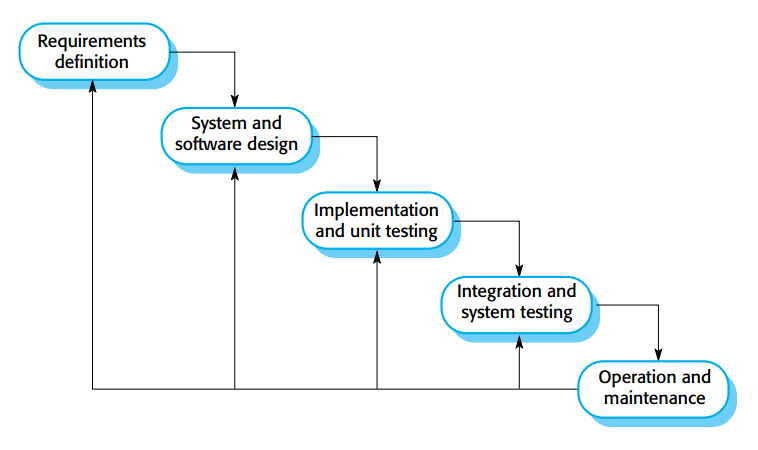
\includegraphics[width=.7\linewidth]{img/waterfall}
  \caption{Model \emph{waterfall} \parencite{sommerville2016software}}\label{fig:waterfall}
\end{figure}

\subsection{Arsitektur \emph{Model View Controller}}

\emph{Model-View-Controller (MVC)} merupakan sebuah model
infrastruktur yang memisahkan antara \emph{user interface} dari
fungsionalitas inti sistem. \emph{Model} memuat segala
\emph{content} dan fungsionalitas yang spesifik pada sistem yang
dibangun, \emph{processing logic} dan akses ke sumber informasi atau
data eksternal. \emph{View} memuat segala fungsi spesifik
\emph{interface}, dan segala proses fungsionalitas yang dibutuhkan
\emph{end-user}. \emph{Controller} mengatur akses ke
\emph{model} dan \emph{view} serta mengatur aliran data antara
keduanya \parencite{pressman2010software}. Penggunaan arsitektur \emph{MVC} akan
menghasilkan tiga \emph{class} utama, yaitu \emph{class view, model},
dan \emph{class controller}. \emph{Class model} akan memuat seluruh
fungsionalitas inti yang spesifik pada sistem. Hal ini memberikan
banyak keuntungan tatkala sistem akan dikembangkan lebih lanjut,
karena pada pengembangan selanjutnya pengembang cukup fokus pada bagian
\emph{controller} dan \emph{view}.

\subsection{Pendekatan Berorientasi Objek}

% sejarah, apa itu pendekatan berorientasi objek ?
Langkah awal yang signifikan terhadap desain berorientasi objek
terlahir dalam komunitas pengguna bahasa pemrograman \emph{Ada}. Hal
ini bermula ketika Grady Booch merasionalkan metode yang diciptakan
Russell J. Abbott pada tahun 1983. Grady Booch kemudian menyebut
karyanya sebagai \emph{object-oriented design}. Keduanya
merekomendasikan bahwa untuk memulai membangun desain berorientasi
objek, dimulai dari deskripsi informal dari sistem yang
akan dibangun. Dari deskripsi informal tersebut pengembang
sistem dapat mengidentifikasi \emph{class} dan objek dari kata benda dan
operasi dari kata kerja yang ditemukan. Beberapa waktu setelahnya
Grady Booch mengemukakan konsep baru yang tidak lagi berbasis pada
deskripsi naratif melainkan menggabungkan \emph{object-oriented
  design} dengan metodologi yang sudah ada, kemudian menyebutnya
sebagai \emph{object-oriented development}
\parencite{capretz2003history}.

Pada tahun 1990-an Grady Booch bersama dengan dua orang rekannya, yaitu
James Rumbaugh dan Ivar Jacobson mulai mengerjakan suatu metode yang
diharapkan bersifat universal. Metode tersebut dibangun berdasarkan
kombinasi dari fitur-fitur terbaik pada metode-metode
\emph{object-oriented analisis} dan \emph{design method} yang
ada. Metode ini juga mengadopsi fitur-fitur yang diajukan oleh ahli
lain dalam rekayasa perangkat lunak. Karya ketiga orang tersebut yang
dikenal sekarang dengan \emph{Unified Modeling
  Language} (\emph{UML}). \emph{UML} berisi notas-notasi yang dapat digunakan
untuk pemodelan dan pengembangan sistem berorientasi objek. Tujuh
tahun setelahnya, yaitu pada tahun 1997 \emph{UML} menjadi standar \emph{de
  facto} untuk membangun perangkat lunak berorientasi objek
\parencite{pressman2010software}.

Membangun perangkat lunak dengan pendekatan berorientasi objek
memiliki aktivitas \emph{object oriented analysis (OOA)} yang di
dalamnya terdapat proses ekstraksi \emph{class} atau \emph{object} dari
pernyataan kebutuhan. Selanjutnya terdapat aktivitas
\emph{object oriented design (OOD)} yang di dalamnya terdapat proses
\emph{refine} dan \emph{extend} \emph{class} yang didapatkan dari
\emph{OOA}. Dalam pengembangan ini umumnya terdapat \emph{boundary
  class} dan \emph{controller class}. \emph{Boundary class} bertindak
sebagai pembatas atau \emph{interface} antara pengguna dan
sistem. \emph{Boundary class} bertanggung jawab mengatur cara sebuah
entitas \emph{object} direpresentasikan kepada
pengguna. \emph{Controller class} mengatur pembuatan atau pembaharuan
pada entitas \emph{object}, penghubung antar \emph{boundary} dan data
yang didapatkan, dan komunikasi antar \emph{object} \parencite{pressman2010software}.


\subsection{Pemodelan Berorientasi Objek}

Notasi yang digunakan untuk pemodelan berorientasi objek adalah
\emph{Unified Modeling Language} (\emph{UML}). \emph{UML} merupakan
standar \emph{de facto} dalam pemodelan berorientasi objek. Terdapat
beberapa diagram inti dalam \emph{UML}, diantaranya adalah \emph{use
  case diagrams, sequence diagrams} dan \emph{class
  diagrams}. \emph{Use case diagrams} menunjukkan interaksi antar
pengguna dan sistem secara visual. \emph{Sequence diagrams}
menunjukkan interaksi antar komponen atau objek di dalam
sistem. \emph{Class diagrams} menunjukkan struktur sistem dan relasi antar
komponen pada sistem  \parencite{sommerville2016software}.

\subsubsection{\emph{Use Case Diagram}}

\emph{Use case diagram} merupakan sebuah diagram statis yang
menggambarkan interaksi antara pengguna dan sistem secara visual. \emph{Use case
  diagram} membantu menentukan fungsionalitas sebuah sistem dari
sudut pandang pengguna~\parencite{pressman2010software}. \emph{Use
  case diagram} tidak menggambarkan tahapan. \emph{Use case}
digambarkan dengan bentuk oval dan aktor digambarkan dengan gambar
orang (\emph{stick figure}). Notasi \emph{use case diagram}
dan deskripsinya dipaparkan pada Tabel~\ref{tab:notasi-use-case},
dan contoh \emph{use case diagram} terdapat dalam
Gambar~\ref{fig:contoh-use-case}.

\begin{longtable}{|>{\centering}m{5cm}|m{7cm}|}
  \caption{Notasi \emph{use case diagram} \parencite{rumbaugh2004unified}}\label{tab:notasi-use-case}
  \\\hline
  \textbf{Notasi} & \textbf{Deskirpsi} \\\hline
  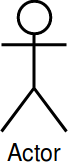
\includegraphics[width=.1\linewidth]{img/uml-notation/actor}
                         & Notasi aktor menggambarkan pengguna atau
                           sistem luar yang berinteraksi dengan
                           sistem. \\\hline
                           %
  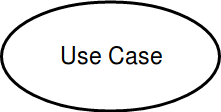
\includegraphics[width=.4\linewidth]{img/uml-notation/usecase}
                         & Notasi \emph{use case} merepresentasikan
                           fungsionalitas yang dapat dijalankan oleh
                           aktor. \\\hline
                           %
  
\includegraphics[width=.6\linewidth]{img/uml-notation/path}
                         & Notasi asosiasi merupakan jalur komunikasi
                           antara aktor dan \emph{use case}. \\\hline
                           %
  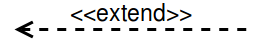
\includegraphics[width=.6\linewidth]{img/uml-notation/extends}
                         & Notasi \emph{extends} merupakan sisipan
                           fungsionalitas tambahan terhadap \emph{base
                           use case} yang tidak mengetahui sisipan
                           tersebut. \\\hline
                           %
  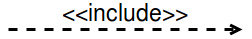
\includegraphics[width=.6\linewidth]{img/uml-notation/include}
                         & Notasi \emph{include} merupakan sisipan
                           fungsionalitas tambahan terhadap
                           \emph{basecase} yang secara eksplisit
                           menjelaskan sisipan tersebut. \\\hline
                           %
  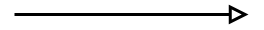
\includegraphics[width=.6\linewidth]{img/uml-notation/general}
                         & Notasi \emph{use case generalization}
                           merupakan relasi antara \emph{general use
                           case} dan \emph{specific use case} yang
                           mewarisi dan menambahkan fitur padanya. \\\hline
\end{longtable}

\begin{figure}[tph]
  \centering
  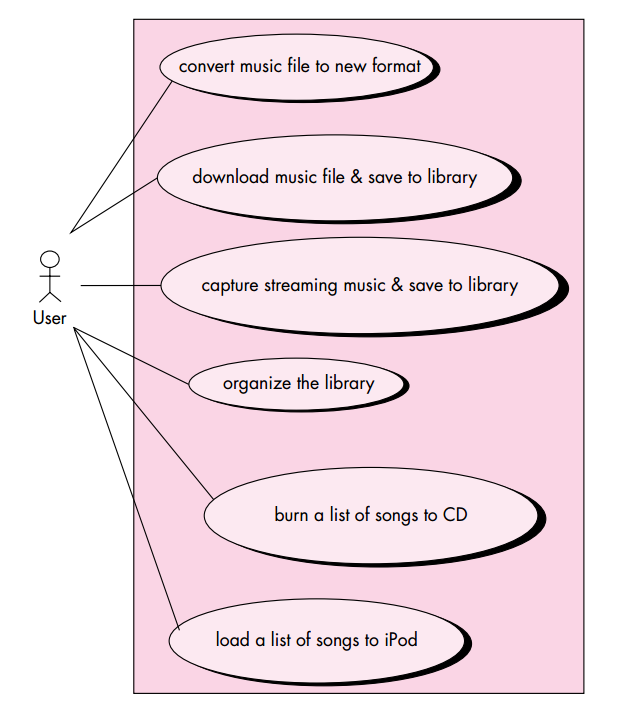
\includegraphics[width=.5\linewidth]{img/contoh-use-case}
  \caption{Contoh \emph{use case diagram} \parencite{pressman2010software}}\label{fig:contoh-use-case}
\end{figure}


\subsubsection{\emph{Sequence Diagram}}

\emph{Sequence diagram} merupakan sebuah diagram dinamis yang
menggambarkan interaksi antar objek di dalam sistem pada saat sistem
mengeksekusi sebuah tugas. Terjadi pertukaran \emph{messages} antar
objek pada sistem untuk menyelesaikan sebuah tugas
\parencite{pressman2010software}. Notasi \emph{sequence diagram} dan
deskripsinya terdapat pada Tabel~\ref{tab:notasi-sequence-diagram},
dan contoh \emph{sequence diagram} terdapat dalam
Gambar~\ref{fig:contoh-sequence-diagram}.

\begin{longtable}{|>{\centering}m{5cm}|m{7cm}|}
  \caption{Notasi \emph{sequence diagram}}\label{tab:notasi-sequence-diagram}\\
  \hline \textbf{Notasi} & \textbf{Deskirpsi} \\\hline
  
\includegraphics[width=.007\linewidth]{img/uml-notation/lifeline}
                         & Notasi \emph{lifeline} menggambarkan waktu
                           aktif (\emph{life}) suatu objek.\\\hline
                           %
  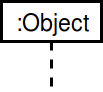
\includegraphics[width=.2\linewidth]{img/uml-notation/objek}
                         & Notasi \emph{object} merepresentasikan objek
                           yang berinteraksi dengan objek lainnya. \\\hline
                           %
  
\includegraphics[width=.04\linewidth]{img/uml-notation/activation-bar}
                         &Notasi \emph{activation bar}
                           merepresentasikan lama suatu objek aktif
                           berinteraksi.\\\hline
                           %
  
\includegraphics[width=.6\linewidth]{img/uml-notation/invoke}
                         & Notasi \emph{method invocation}
                           merepresentasikan suatu \emph{method} dari
                           sebuah objek yang panggil oleh objek
                           lainnya.\\\hline
                           %
  
\includegraphics[width=.6\linewidth]{img/uml-notation/return}
                         & Notasi \emph{return} merepresentasikan data
                           yang dikembalikan oleh method \emph{calle}
                           kepada method \emph{caller}.\\\hline
                           %
  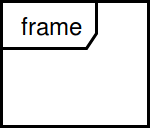
\includegraphics[width=.4\linewidth]{img/uml-notation/frame}
                         & Notasi \emph{frame} menggambarkan lingkup
                           suatu interaksi dengan interaksi lainnya
                           atau lingkup suatu interaksi dan dunia luar. \\\hline
                         %
  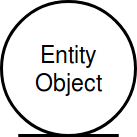
\includegraphics[width=.3\linewidth]{img/uml-notation/entity}
                         & Notasi \emph{entity object} merepresentasikan
                           objek yang bertanggung jawab untuk mengatur
                           data dalam sebuah sistem. \\\hline
                         %
  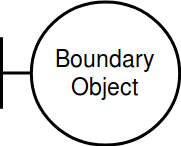
\includegraphics[width=.3\linewidth]{img/uml-notation/boundary}
                         & Notasi \emph{boundary object} merepresentasikan
                           objek yang bertanggung jawab untuk mengatur
                           alur sebuah objek direpresentasikan kepada aktor. \\\hline
                         %
  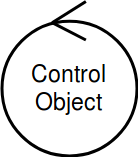
\includegraphics[width=.3\linewidth]{img/uml-notation/control}
                         & Notasi \emph{controller object}
                           merepresentasikan suatu objek yang mengatur
                           pembuatan atau pembaharuan entitas
                           \emph{object}, penghubung antar
                           \emph{boundary} dan \emph{entity} dan
                           komunikasi antar \emph{object}. \\\hline

\end{longtable}

\begin{figure}[tph]
  \centering
  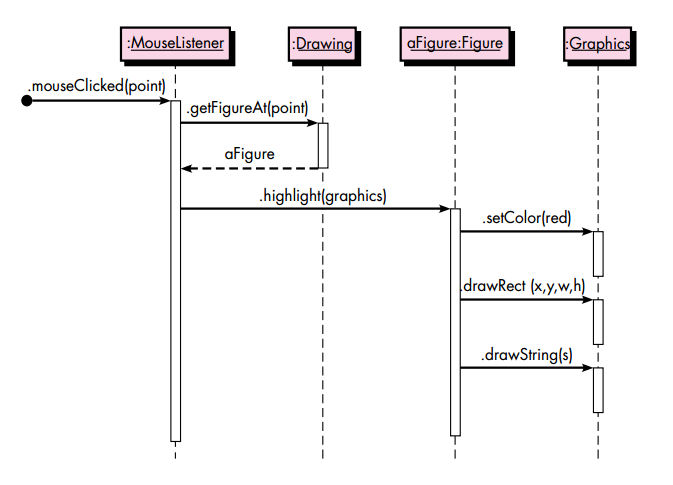
\includegraphics[width=.7\linewidth]{img/contoh-sequence}
  \caption{Contoh \emph{sequence diagram} \parencite{pressman2010software}}
   \label{fig:contoh-sequence-diagram}
\end{figure}


\subsubsection{\emph{Class Diagram}}

\emph{Class diagram} merupakan sebuah diagram statis atau \emph{structural view}
yang memodelkan \emph{class}, \emph{class attribute}, \emph{class operation},
hubungan, dan asosiasi antar \emph{class}. Elemen utama dari \emph{class
  diagram} adalah kotak yang terbagi menjadi beberapa bagian. Bagian atas
merepresentasikan nama \emph{class}, bagian tengah merepresentasikan
\emph{attribute}, dan bagian bawah merepresentasikan
\emph{operation}. \emph{Attribute} merupakan apa yang sebuah \emph{class} atau
objek ketahui, \emph{operation} merupakan apa yang sebuah \emph{class} atau
objek dapat lakukan~\parencite{pressman2010software}. Notasi dan deskripsi dari
notasi tersebut dipaparkan pada Tabel~\ref{tab:notasi-class-diargam}, dan Contoh
dari \emph{class diagram} terdapat dalam Gambar~\ref{fig:contoh-class-diagram}.

\begin{longtable}{|>{\centering}m{5cm}|m{7cm}|}
  \caption{Notasi \emph{class diagram}}\label{tab:notasi-class-diargam}\\
  \hline \textbf{Notasi} & \textbf{Deskirpsi} \\\hline
  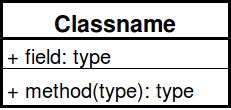
\includegraphics[width=.44\linewidth]{img/uml-notation/class}
                         & Notasi \emph{class} merepresentasikan suatu
                           \emph{class} yang berisikan
                           \emph{attribute} dan \emph{method}.\\\hline
                           %
  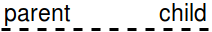
\includegraphics[width=.6\linewidth]{img/uml-notation/association-class}
                         & Notasi \emph{association} menggambarkan
                           hubungkan antar suatu \emph{class} dengan
                           \emph{class} lainnya. \\\hline
                           %
  
\includegraphics[width=.6\linewidth]{img/uml-notation/composition-class}
                         & Notasi \emph{composition} menggambarkan
                           hubungan kuat antar suatu \emph{class} dengan
                           \emph{class} lain, di mana keduanya
                           saling membutuhkan secara kuat dan saling
                           membutuhkan. \\\hline
                           %
  
\includegraphics[width=.6\linewidth]{img/uml-notation/agregation-class}
                         & Notasi \emph{agregation} menggambarkan
                           hubungan lemah antar suatu \emph{class}
                           dengan \emph{class} yang lain, di mana
                           keduanya tidak saling membutuhkan atau keduanya bisa
                           berdiri sendiri. \\\hline
                           %
  
\includegraphics[width=.6\linewidth]{img/uml-notation/generalization-class}
                         & Notasi \emph{generalization}
                           merupakan relasi antara \emph{parent class}
                           dan \emph{child class}, di mana \emph{child class}
                           mewarisi dan menambahkan fitur dari
                           \emph{parent class}. \\\hline
                           %
\end{longtable}

\begin{figure}[tph]
  \centering
  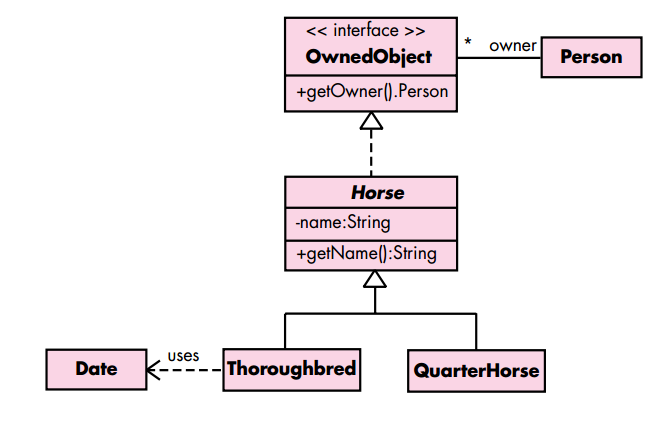
\includegraphics[width=.6\linewidth]{img/contoh-class}
  \caption{Contoh \emph{class diagram} \parencite{pressman2010software}}
  \label{fig:contoh-class-diagram}
\end{figure}


\subsection{Pengujian Perangkat Lunak}

% kapan pengujian itu ada
% apa kekurangan dan kelebihan
% metode yang digunakan apa aja

Penggunaan perangkat lunak yang masif tanpa adanya standardisasi
membuat \emph{IEEE} mempublikasikan sebuah \emph{issue} pada bulan november
hingga desember di tahun 1999. \emph{IEEE} dan \emph{ACM} kemudian
membentuk tim gabungan untuk mendefinisikan standardisasi pada proses
pengembangan perangkat lunak. Standardisasi tersebut memuat tentang
\emph{scientific principles, engineering processes, standards,
  methods, tools, measurement} dan \emph{best practices}, proses pengujian
atau \emph{testing} termasuk di dalamnya \parencite{burnstein2006practical}.

Pengujian bertujuan untuk menemukan cacat dan menguji kualitas suatu
perangkat lunak. Dalam proses pengujian terdapat beberapa tahapan, metode, dan
teknik. Setiap komponen pada bagian-bagian tersebut memiliki
kelemahan dan kekurangan tertentu. Proses testing juga akan
menghasilkan artefak-artefak seperti \emph{test-scenario, test-case,
  test-data} dan \emph{test scripts} \parencite{burnstein2006practical}.

\subsubsection{Tahapan Pengujian}

Terdapat beberapa tahapan dalam pengujian. Tahapan-tahapan tersebut
diantaranya \emph{unit testing, integration testing}, dan \emph{validation
  testing} \parencite{presman2010software}. Tahapan awal dalam pengujian adalah
tahapan pengujian \emph{unit}. Terdapat beberapa
pendapat berbeda mengenai ``\emph{unit}'' dalam \emph{unit
  testing}. \textcite{martin2014unittest} berpendapat bahwa definisi
\emph{unit} dapat berarti \emph{single method, single class} maupun
kumpulan dari beberapa \emph{class}. \textcite{osherove2015art} tidak
mengikat definisi \emph{unit} pada \emph{class} maupun
\emph{method}, melainkan mengikatnya dengan definsi atribut seperti
\emph{performance, reliability} dan \emph{consistency}. \emph{Google}
tidak menggunakan istilah \emph{unit, integration} ataupun
\emph{system} untuk merujuk pada tingkatan tertentu, melainkan
menggunakan istilah \emph{small, medium, large}
\parencite{whittaker2012google}. Di sisi lain,
\textcite{presman2010software} berpendapat bahwa fokus pengujian
\emph{unit} pada perangkat lunak konvensional adalah sebuah modul dan
fokus pengujian \emph{unit} pada perangkat lunak berorientasi objek
adalah \emph{class} dengan \emph{testable unit} terkecil adalah
\emph{operation} atau \emph{method}. Tahapan selanjutnya adalah \emph{Integration
  testing}. \emph{Integrartion testing} merupakan pengujian yang
dilakukan pada kumpulan \emph{unit} yang telah diuji. Hal ini
dilakukan untuk memastikan suatu \emph{unit} akan berjalan dengan baik
jika dijalankan bersamaan dengan \emph{unit} yang lain. Meskipun
setiap \emph{unit} telah diuji secara individu, terdapat beberapa
kemungkinan galat yang terjadi ketika \emph{unit-unit} tersebut diuji
secara bersamaan. Beberapa kemungkinan galat yang akan terjadi di
antaranya adalah hilangnya data ketika melintasi \emph{interface}, dan
komponen yang tidak berjalan semestinya ketika digabungkan. Pada
proses pengujian \emph{unit} maupun \emph{integrartion}, komponen
tidak berupa \emph{stand-alone program}. Maka dibutuhkan pembuatan
\emph{stub} ataupun \emph{driver} selama proses pengujian.
\emph{Driver} hanyalah \emph{main program} tiruan yang menjalankan
kasus uji, sedangkan \emph{stub} merupakan sebuah \emph{dummy
  subprogram} yang bekerja menggantikan komponen-komponen pengujian
yang asli.

Pada sistem dengan arsitektur berorientasi objek pengujian integrasi
dengan pendekatan \emph{incremental top-down integration} maupun
\emph{incremental bottom-up integration} tidak dapat digunakan,
karena sistem berorientasi objek tidak memiliki kontrol hierarki
yang jelas. Maka dibutuhkan pendekatan yang berbeda, yaitu dengan
pendekatan integrasi \emph{thread-based testing} dan \emph{use-based
  testing}. \emph{Thread-based testing} bekerja dengan
mengintegrasikan sekumpulan \emph{class} yang dibutuhkan untuk \emph{input}
tertentu. Setiap \emph{thread} diuji dan diintegrasikan secara
individu. \emph{Use-based testing} berkeja dengan menguji
\emph{class} independen yang memiliki ketergantungan paling kecil
dengan \emph{class} lainnya. Setelah \emph{class}-\emph{class}
tersebut diuji, lapisan \emph{class} selanjutnya (\emph{dependent
  classess}) yang menggunakan \emph{independent class} diuji hingga
seluruh sistem selesai diuji \parencite{presman2010software}. Tahapan terakhir adalah pengujian
validasi atau \emph{validation testing}. Pengujian validasi fokus
terhadap \emph{user-visible action} dan \emph{user-recognizable
  output} dari sistem, atau dengan kata lain pengujian validasi
menguji apakah sistem yang dibangun sudah sesuai dengan seluruh
skenario kebutuhan yang didefinisikan~\parencite{pressman2010software}. Tahapan pengujian
terlihat dalam Gambar~\ref{fig:testing-level}.

\begin{figure}[H]
  \centering
  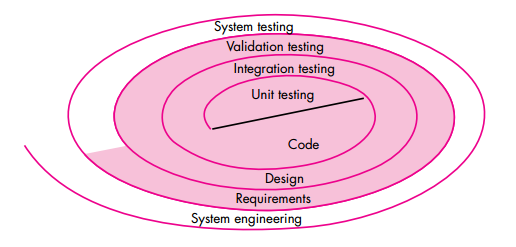
\includegraphics[width=.7\linewidth]{img/tahapan-pengujian}
  \caption{Tahapan pengujian \parencite{presman2010software}}\label{fig:testing-level}
\end{figure}

\subsubsection{Metode Pengujian}

Metode pengujian atau \emph{point of view} dalam pengujian merupakan
sudut pandang seorang \emph{tester} tatkala mendesain sebuah
\emph{test case}. Terdapat di antaranya \emph{white-box testing} dan
\emph{black-box testing}. Kedua metode tersebut memiliki kekurangan
masing-masing. Metode \emph{white-box testing} tidak dapat menemukan
kebutuhan yang belum diimplementasikan
\parencite{dijkstra1970notes}. Hal ini dapat diselesaikan dengan
penggunaan metode \emph{black-box testing}. Begitu juga dengan
kekurangan metode \emph{black-box testing} yang dapat menghasilkan
\emph{test-case} yang tidak tepat dan tidak dapat menemukan bagian
yang belum diuji \parencite{savenkov2008become}. Kelemahan pada metode
\emph{black-box testing} ini dapat diselesaikan dengan menggunakan
metode \emph{white-box testing}. Oleh karena itu, penggunaan kedua metode
dalam pengujian sistem menyelesaikan semua masalah pada masing-masing kekurangan
yang dimiliki kedua metode.

\emph{White-box testing} merupakan suatu metode pengujian di mana
proses pengujiannya dilakukan dengan melihat internal perangkat lunak.
Maka pada tahapan ini seorang penguji wajib memiliki kemampuan
pemrograman. Pengujian ini dilakukan untuk menguji apakah \emph{logic}
dan \emph{data} pada perangkat lunak berfungsi sebagaimana mestinya
\parencite{myers2011art}. Di sisi lain \emph{black-box testing} hanya
menguji bagian luar suatu perangkat lunak. Pada tahapan ini
fungsionalitas suatu perangkat lunak diuji tanpa harus mengetahui
internalnya. Oleh karena itu, tidak dibutuhkan kemampuan pemrograman
saat membuat \emph{test case} pada pengujian \emph{black-box}. Penguji
hanya mengetahui bagaimana seharusnya perangkat lunak berjalan
(\emph{what}), bukan bagaimana perangkat lunak itu melakukan sesuatu
(\emph{how}). Pada tahapan ini penguji hanya mempertimbangkan masukan
(\emph{input}) dan keluaran (\emph{output}) perangkat lunak selama
mendesain \emph{test-case} \parencite{myers2011art}.


\subsubsection{Teknik Pengujian}

Terdapat beberapa teknik dalam pengujian. Pengujian semua \emph{path}
atau \emph{rigorous testing} pada proses \emph{white-box testing}
tidak mungkin dilakukan sehingga digunakan teknik \emph{basis path
testing} untuk menentukan \emph{path} yang akan diuji
\parencite{gregory2007path}. \emph{Rigorous testing} atau
\emph{exhaustive testing} (\emph{C$\infty$}) atau menguji semua
kemungkinan juga tidak mungkin dilakukan pada saat pengujian
\emph{black-box} sehingga penggunaan teknik \emph{equivalence
partitioning} untuk menentukan masukan yang \emph{valid} dan
\emph{invalid} diperlukan. Teknik \emph{boundary value analysis}
menjadi pelengkap teknik \emph{equivalence
partitioning}. \emph{Boundary value analysis} digunakan untuk
mendapatkan nilai masukan yang berada pada \emph{boundary} atau
\emph{corner}, karena nilai-nilai pada bagian tersebut memiliki
kemungkinan galat yang besar \parencite{presman2010software}. Maka tiga teknik
utama dalam pengujian perangkat lunak adalah:

\begin{enumerate}
\item \emph{Basis path testing}
\item \emph{Equivalence partitioning}
\item \emph{Boundary value analysis }
\end{enumerate}

\emph{Basis path testing} merupakan suatu teknik pengujian pada metode
\emph{white-box} yang diajukan oleh McCabe pada tahun 1996. Teknik ini
menggunakan penelitian McCabe yang sebelumnya yaitu \emph{cyclomatic
complexity} yang ia temukan pada tahun 1976. Meski saat ini \emph{cyclomatic
complexity} banyak dikaitkan secara erat dengan rumus untuk menentukan
jumlah \emph{independent path}. \emph{Cyclomatic complexity} yang awalnya
ditemukan pada tahun 1976 diajukan untuk mengukur tingkat kompleksitas
suatu modul dalam sebuah program. Modul yang melebihi nilai
\emph{cyclomatic complexity} sepuluh direkomendasikan untuk dipisah atau
dilakukan \emph{refactoring}. Tujuan kedua dari rumus tersebut adalah
untuk melihat tingkat terstrukturnya (\emph{structuredness}) suatu
modul. Hal yang membuat \emph{cyclomatic complexity} dikaitkan secara
erat dengan proses \emph{basis path testing} karena kemudian McCabe
sadar bahwa \emph{cyclomatic complexity} dapat menemukan
\emph{independent path} pada suatu modul. \emph{Independent path} adalah
suatu jalur dalam sebuah program yang memperkenalkan setidaknya suatu rangkaian
pemrosesan baru atau kondisi baru. Hal tersebut yang
mengantarnya pada pengajuan \emph{basis path testing} pada tahun 1996.
\emph{Basis path testing} memiliki keunggulan karena V(G) atau
\emph{vector space} memiliki nilai yang menjadi batas atas \emph{upper
bound} untuk membuat \emph{test-case} pada suatu program. Hal ini
menguntungkan penguji karena dapat menentukan ukuran batas selesainya
suatu pengujian. Selain itu, \emph{basis path testing} memiliki nilai
yang lebih baik dari pada \emph{branch coverage}, yaitu \emph{branch
  coverage ≤ cyclomatic complexity ≤ all of paths} \parencite{gregory2007path}.
Langkah-langkah pengujian \emph{basis path} adalah sebagai berikut \parencite{presman2010software}:

\begin{enumerate}[
leftmargin=0pt, itemindent=20pt,
labelwidth=15pt, labelsep=5pt, listparindent=0.7cm,
align=left]
\item Membuat \emph{flow graph} dari desain atau \emph{code}.

  \emph{Flow graph} memiliki beberapa notasi seperti \emph{sequence,
    if, while, until} dan \emph{case}. Gambar notasi-notasi tersebut
  terlihat pada Gambar~\ref{fig:notasi-flow-graph}. Terlihat \emph{flow graph}
  pada Gambar~\ref{cfg:hallo} yang dihasilkan dari
  \emph{pseudocode}~\ref{ps:hallo}.

\item Menentukan \emph{cyclomatic complexity} dari \emph{flow graph}
  yang dihasilkan.

  \emph{Cyclomatic complexity} adalah suatu metrik perangkat lunak
  yang memberikan ukuran kuantitatif kompleksitas logis dari suatu
  program. \emph{Cyclomatic complexity} dapat ditentukan dengan menggunakan
  rumus~\ref{eq:perhitungan-cc}:

  \begin{equation}
    \begin{array}{l}
      V(G) = jumlah \thinspace region \\
      V(G) = E – N + 2 \\
      V(G) = P + 1, \thinspace di mana \thinspace P – predicate \thinspace node
    \end{array}\label{eq:perhitungan-cc}
  \end{equation}

  Maka Perhitungan \emph{cyclomatic complexity} yang dilakukan pada
  \emph{flow graph}~\ref{cfg:hallo} menghasilkan
  nilai sebagai berikut:

  \begin{equation}
    \begin{array}{l}
      V(G) = 2 \thinspace regions \\
      V(G) = 4 \thinspace edges \thinspace – \thinspace 4 \thinspace
      nodes \thinspace + \thinspace 2 \thinspace = \thinspace 2 \\
      V(G) = 1 \thinspace predicate \thinspace node \thinspace +
      \thinspace 1 \thinspace = \thinspace 2
    \end{array}\label{eq:hasil-perhitungan-cc}
  \end{equation}

 Jadi, \emph{flow graph} pada Gambar~\ref{cfg:hallo} memiliki nilai
 \emph{cyclomatic complexity} = 2.

\item Menentukan \emph{independent path}.

  \emph{Independent path} adalah suatu jalur dalam sebuah program yang
  memperkenalkan setidaknya suatu rangkaian pemrosesan baru atau
  kondisi baru. Nilai dari V(G) memberikan batas atas dari banyaknya
  \emph{independent path} dari sebuah program. Dari contoh
  \emph{pseudocode} \emph{procedure hallo} kita mendapatkan 2 jalur
  \emph{independent} sebagai berikut: \par\null\par

  Jalur 1: 1 - 2 - 4 \par
  Jalur 2: 1 - 3 - 4

\item Membuat \emph{test case} yang akan menjalankan setiap jalur pada
  \emph{basis path}.

  Terdapat dua \emph{test case} yang akan dihasilkan. Pertama
  \emph{test case} yang harus melewati jalur 1 sehingga pada \emph{test
    case} pertama nilai \emph{variable nama} harus bernilai
  \emph{true}. Pada \emph{test case} kedua nilai \emph{variable nama}
  harus bernilai \emph{false} agar jalur 2 dijalankan. \emph{Test case}
  yang dihasilkan tampak seperti pada Tabel~\ref{tc:hallo}.

\end{enumerate}

\begin{figure}[H]
  \centering
  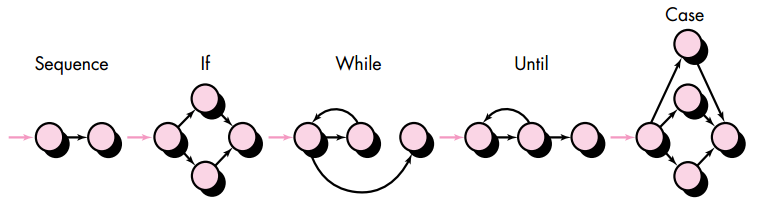
\includegraphics[width=.8\linewidth]{img/notasi-flow-graph}
  \caption{Notasi \emph{flow graph} \parencite{presman2010software}}\label{fig:notasi-flow-graph}
\end{figure}


\begin{center}
\begin{minipage}{0.8\textwidth}
\begin{code}
\begin{ignasicblock}[title=hallo,minted language=text]
procedure hallo(nama)
   IF nama == "Budi"          (1)
      RETURN "Hai" + nama     (2)
   ELSE
      RETURN "Nama kosong"    (3)
   ENDIF                      (4)
end
\end{ignasicblock}
\captionof{listing}{Contoh \emph{pseudocode}}\label{ps:hallo}
\end{code}
\end{minipage}
\end{center}

\begin{figure}[H]
  \centering
  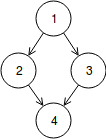
\includegraphics[width=.14\linewidth]{img/contoh-flow-graph}
  \caption{Representasi \emph{control flow graph} dari \emph{pseudocode}~\ref{ps:hallo}}\label{cfg:hallo}
\end{figure}

\begin{longtable}{|P{.06\textwidth}|P{.30\textwidth}|P{.30\textwidth}|P{.10\textwidth}|P{.08\textwidth}|}
  \caption{\emph{Test case} dari contoh \emph{pseudocode}~\ref{ps:hallo}} \label{tc:hallo}\\
  \hline
  \textbf{Jalur} & \textbf{Prosedur Uji} & \textbf{\emph{Expected Result}} \\\hline
  %
  1 & Memberikan nilai \emph{``Budi''} pada variable \emph{nama} &
                                                                   Program menampilkan ``Hai Budi'' \\\hline
                                                                   %
  2 & Tidak memberikan nilai apapun pada variable \emph{nama} &
                                                                   Program menampilkan ``Nama kosong'' \\\hline
  %

\end{longtable}


\emph{Equivalence partitioning} merupakan suatu teknik dalam metode
pengujian \emph{black-box} di mana prosesnya adalah membagi masukan
kepada kelas-kelas data. Dari kelas-kelas tersebut \emph{test case}
nantinya didapatkan. \emph{Equivalence class} merepresentasikan
keadaan valid atau tidak validnya suatu masukan. Beberapa kondisi
masukan di antaranya \emph{numeric value, range of values, set of
related values,} atau \emph{boolean condition}. \emph{Equivalence
partitioning} dapat di definisikan sesuai dengan panduan berikut
\parencite{presman2010software}:

\begin{enumerate}[
leftmargin=0pt, itemindent=20pt,
labelwidth=15pt, labelsep=5pt, listparindent=0.7cm,
align=left]

\item Jika kondisi masukan adalah \emph{range}. Maka satu valid dan
  dua invalid \emph{equivalence class} di definisikan.
\item Jika kondisi masukan adalah \emph{specific value}. Maka satu valid dan
  dua invalid \emph{equivalence class} di definisikan.
\item Jika kondisi masukan adalah \emph{member of a set}. Maka satu valid dan
  satu invalid \emph{equivalence class} di definisikan.
\item Jika kondisi masukan adalah \emph{boolean}. Maka satu valid dan
  satu invalid \emph{equivalence class} di definisikan.

\end{enumerate}

Jika data masukan bertipe \emph{range} dan masukan yang valid adalah
\emph{range} bernilai 4 hingga 10. Maka masukan yang tidak valid
adalah semua angka yang kurang dari 4 dan semua angka yang lebih dari
10 seperti terlihat pada Gambar~\ref{fig:contoh-ep-marked}. Data
yang digunakan untuk \emph{test case} pada tipe masukan \emph{range}
berjumlah 3. Satu bernilai valid dan dua bernilai invalid. Oleh karena itu,
data masukan \emph{valid} yang kita gunakan adalah 11 dan 7. Sedangkan
data \emph{invalid} yang digunakan adalah 3.

\begin{figure}[H]
  \centering
  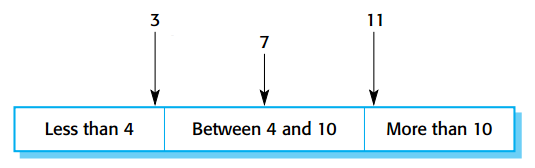
\includegraphics[width=.6\linewidth]{img/contoh-ep-marked}
  \caption{Contoh \emph{equivalence partitioning} \parencite{sommerville2016software}}\label{fig:contoh-ep-marked}
\end{figure}

\emph{Boundary value analysis} merupakan suatu teknik yang melengkapi
\emph{equivalence partitioning}. \emph{Boundary value analysis}
dikembangkan untuk menganalisis nilai yang berada pada \emph{boundary}
\emph{input}, karena nilai pada \emph{boundary} atau \emph{corner} memiliki
peluang galat yang lebih tinggi. \emph{Boundary value analysis} tidak
berdiri sendiri, melainkan merupakan teknik yang melengkapi
\emph{equivalence partitioning}. Maka \emph{boundary value analysis}
mengambil nilai yang bersifat ``pojok'' dari nilai hasil
\emph{equivalence partitioning}. Panduan pemilihan nilai
\emph{boundary value analysis} di antaranya sebagai berikut
\parencite{presman2010software}:

\begin{enumerate}[
leftmargin=0pt, itemindent=20pt,
labelwidth=15pt, labelsep=5pt, listparindent=0.7cm,
align=left]

\item Jika masukan merupakan sebuah \emph{range} dari a hingga
  b. Maka nilai yang digunakan untuk \emph{test case} adalah satu
  nilai di atas a dan satu nilai di bawah b.
\item Jika masukan merupakan sebuah \emph{number of values}. Maka
  nilai yang digunakan untuk \emph{test case} adalah nilai maksimum
  dan minimum serta satu nilai di atas maksimum dan satu nilai di
  bawah minimum.
\end{enumerate}

Jika data masukan bertipe \emph{range} dari 4 hingga 10. Maka nilai
yang didapatkan untuk pengujian adalah nilai maksimum dan minimum
serta satu nilai di atas maksimum dan satu nilai di atas minimum. Jadi
nilai yang didapatkan adalah 4, 10, 3, dan 11 seperti terlihat pada
Gambar~\ref{fig:contoh-bva-marked}.

\begin{figure}[H]
  \centering
  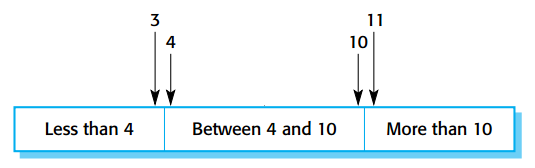
\includegraphics[width=.6\linewidth]{img/contoh-bva-marked}
  \caption{Contoh \emph{boundary value analysis}
    \parencite{sommerville2016software}}\label{fig:contoh-bva-marked}
\end{figure}

\subsubsection{\emph{Automated Testing}}

Menjalankan semua \emph{test case} secara manual sangat menyita
waktu. Bahkan mereka dapat menyita 50\% dari pada waktu pengembangan
\parencite{brooks1995mythical}. \emph{Automated testing} dapat
digunakan untuk mempercepat proses pengujian. \emph{Automated testing}
adalah proses menjalakan \emph{test case} secara otomatis.
\emph{Automated testing} berjalan dengan adanya \emph{trigger}, baik
dalam bentuk \emph{event} maupun \emph{time}. Prosesnya adalah dengan
menjalankan \emph{test case} dan membandingkannya dengan \emph{output}
yang sudah ditentukan. Hasil perbandingan tersebut akan dilaporkan
kepada penguji secara otomatis setelah \emph{automated testing}
selesai dijalankan \parencite{marcellintravis}. \emph{Automated
  testing} dibangun dengan menggunakan \emph{script} sesuai dengan
\emph{test case} yang didapatkan dari tahapan pengujian
\emph{white-box} maupun \emph{black-box}. Tampak pada Tabel
Kode~\ref{ts:hallo} merupakan \emph{script} yang dibangun untuk
melakukan pengujian secara otomatis. \emph{Script} tersebut didapatkan dari
\emph{test case} untuk pengujian \emph{pseudocode hallo} pada Tabel
Kode~\ref{tc:hallo}. \emph{Script} ini nantinya dijalankan dengan
kakas bantu \emph{Pytest} untuk melakukan pengecekan berhasil atau
gagalnya suatu pengujian secara otomatis. Sedangkan \emph{trigger} untuk
menjalankan \emph{Pytest} secara otomatis dilakukan dengan bantuan
kakas bantu \emph{Gitlab-CI}.

\begin{center}
\begin{minipage}{0.8\textwidth}
\begin{code}
\begin{ignasicblock}[title=test\_hallo,minted language=Python]
      def test_case_1():
          assert hallo("Budi") == "Hai Budi"

      def test_case_2():
          assert hallo("Ani") == "Nama Kosong"
\end{ignasicblock}
\captionof{listing}{Contoh \emph{script atomated testing}}\label{ts:hallo}
\end{code}
\end{minipage}
\end{center}

\subsubsection{Pengujian \emph{Compatibility}}

Pengujian \emph{compatibility} adalah pengujian yang dilakukan pada sistem yang
dibangun di atas beberapa media yang berbeda, seperti di atas \emph{display
  devices, operating systems} dan \emph{browser} yang
berbeda-beda. Masalah \emph{compatibility} yang kecil tidak memberikan
dampak signifikan pada sistem, tetapi masalah yang besar dapat
mengakibatkan dampak besar \parencite{pressman2010software}. Terdapat berbagai macam \emph{desktop
  environment} yang berbeda-beda pada sistem operasi \emph{GNU/Linux}. Setiap
\emph{desktop environment} memiliki format nama \emph{window} tersendiri. Sebuah
sistem harus dapat menangani perbedaan format nama \emph{window} agar dapat
\emph{compatible} antar \emph{desktop environment}. Pengujian \emph{compatibility}
terhadap perbedaan format nama \emph{window} antar \emph{desktop environment}
dilakukan dengan menjalankan sistem pada berbagai \emph{desktop environment} yang berbeda. Pengujian
berhasil jika sistem dapat menangani perbedaan format-format tersebut.
Beberapa format nama \emph{window} pada \emph{desktop environment} di antaranya:

\begin{itemize}
\item ``\_NET\_ACTIVE\_WINDOW(WINDOW): window id \# 0x3c00009''
\item ``\_NET\_ACTIVE\_WINDOW(WINDOW): window id \# 0x4a0000c, 0x0''
\end{itemize}

% teori teori apa saja yang dipakai.
%% activity logging, snapshotting, edit distance
\section{\emph{Snapshotting}}

% istilah snapshot sebenarnya datang dari analogi \emph{screenshot}
% dari dunia fotografi.
\emph{Snapshot} merupakan proses untuk merekam suatu keadaan media
penyimpanan dalam suatu waktu tertentu. \emph{Snapshot} yang
dihasilkan dapat dikembalikan kapan pun pengguna butuhkan. Umumnya
\emph{snapshot} dapat dihasilkan dari beberapa kakas bantu seperti
\emph{data protection software, data analisys}, dan \emph{replication
  aplication}. Implementasi untuk melakukan \emph{snapshot}
berbeda-beda, tergantung pada kebutuhan aplikasi\parencite{garimella}.
\emph{Version Control Software} (\emph{VCS})
merupakan salah satu kakas bantu yang dapat digunakan untuk membuat
\emph{snapshot}. \emph{VCS} lahir dimulai dengan adanya \emph{Source Code Control System (SCCS)}
pada tahun 1972 yang dibangun oleh Marc J. Rochkind, disusul
kemunculan \emph{Revision Control System (RCS)} pada tahun 1980,
\emph{Concurrent Versions System (CVS)} pada tahun 1985,
kemudian \emph{subversion} dan \emph{git} pada tahun-tahun berikutnya
\parencite{ruparelia2010history}

% https://git-scm.com/book/en/v2/Appendix-C%3A-Git-Commands-Basic-Snapshotting
\emph{Git} merupakan salah satu \emph{version control software} yang digunakan
secara umum. Hal ini disebabkan karena \emph{git} memiliki sifat
\emph{distributed} sehingga memiliki kelebihan yang tidak dimiliki
\emph{version control} terpusat, salah satunya adalah kemampuan untuk
melakukan seluruh operasi secara lokal \parencite{ruparelia2010history}.
\emph{Snapshot} pada \emph{git} disimpan di dalam \emph{repository} dan digunakan
untuk menyimpan suatu berkas dalam keadaan tertentu. Proses pembuatan \emph{snapshot} dapat
dilakukan dengan meminta \emph{git} untuk menambahkan semua
berkas yang ada menggunakan perintah ``\emph{add}''. Proses selanjutnya dilakukan dengan
menyimpan \emph{snapshot} secara permanen dengan menggunakan perintah
``\emph{commit}''. Proses ini akan menyimpan \emph{snapshot}
secara permanen pada \emph{database} \emph{git}.  Perintah lainnya yang dapat
kita gunakan adalah ``\emph{log}'' untuk melihat \emph{history} dari
\emph{snapshot}, dan ``\emph{diff}'' untuk melihat perbedaan antar
\emph{snapshot} \parencite{chacon2014pro}.

% how object stored Git benar-benar mengubah paradigma dunia e{version
Umumnya \emph{version control} beroperasi dengan menyimpan \emph{diff}
antar berkas pada suatu saat tertentu, cara ini biasa disebut dengan
\emph{delta-based version control}. Hal ini berbeda dengan \emph{git} yang menyimpan
keseluruhan \emph{snapshot} pada suatu waktu tertentu. Setiap
``\emph{commit}'' akan menyimpan seluruh keadaan berkas, kecuali
berkas yang tidak berubah. \emph{Git} melihat \emph{project} layaknya
\emph{stream of snapshots}. Semua \emph{snapshot} tersebut memiliki
integritas yang berupa 40 karakter \emph{hexadecimal} dihasilkan dari
kalkulasi berkas pada suatu \emph{snapshot} dengan algoritme
\emph{SHA-1}. Dengan \emph{hash} tersebut, \emph{git} dapat merujuk
suatu \emph{snapshot} tertentu \parencite{chacon2014pro}.

\begin{figure}[tph]
  \centering
  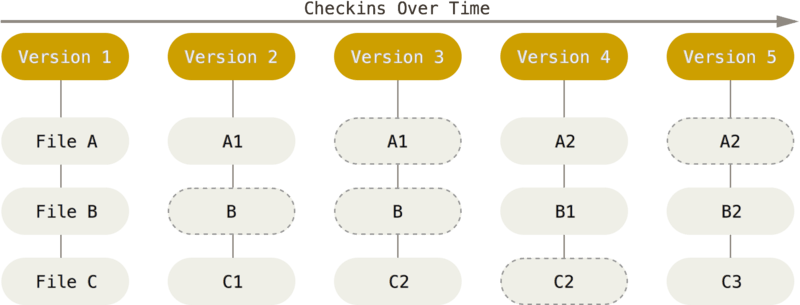
\includegraphics[width=.7\linewidth]{img/snapshots}
  \caption{Penyimpanan data sebagai \emph{snapshot} dari waktu ke
    waktu~\parencite{chacon2014pro}}\label{fig:snapshots}
\end{figure}


\section{\emph{User Activity Logging}}

% apa itu log ?
\emph{Log} merupakan sebuah berkas yang memuat rekaman semua aktivitas
yang terjadi pada perangkat lunak yang sedang berjalan. Pada
umumnya \emph{log} memiliki format berupa \emph{plain text} dan memuat
informasi berupa waktu, kategori dan deskripsi. \emph{Log} secara umum
digunakan pada \emph{web server, operating system} dan berbagai macam
perangkat lunak lain. Merekam aktivitas perangkat lunak maupun
pengguna dan menyimpannya ke dalam \emph{log} bertujuan untuk
melakukan \emph{debugging, monitoring, optimization, forensic
  analysis} dan beberapa tujuan lain. \emph{Log} memiliki beberapa
macam tipe, di antaranya \emph{event logs, message logs} dan
\emph{transaction log} \parencite{delarosa}.

% apa itu user activity logging ?
\emph{User activity logging} adalah sebuah proses menyimpan aktivitas pengguna ke dalam
sebuah \emph{log}. \emph{User activity} merupakan aktivitas pengguna dalam menggunakan
perangkat lunak. \emph{User activity} diantaranya adalah \emph{keystrokes}, gerakan
\emph{mouse}, suara, gerakan, gerakan mata, tempat yang dikunjungi, berkas yang dibuka,
dan aplikasi yang dijalankan \parencite{macbeth2007logging}.

\section{\emph{Edit-distance Algorithm}}

\emph{Edit-distance} merupakan algoritme yang melakukan perhitungan
pada penghapusan, sisipan, maupun substitusi antara dua buah
kata. Algoritme ini lebih umum dikenal dengan \emph{edit
  distance}, tetapi umumnya \emph{edit distance} merujuk pada
\emph{levenshtein distance}. Algoritme ini ditemukan oleh
matematikawan rusia, Vladimir Levenshteinn pada 1965. Pada algoritme
ini semua karakter yang ada, memiliki \emph{unit cost} (harga yang
nantinya dikalkulasi) kecuali substitusi yang dilakukan pada karakter
itu sendiri. Secara umum algoritme ini memiliki nilai yang sama dengan
nilai minimal operasi yang diperlukan untuk mengubah karakter ``a''
menjadi ``b'' \parencite{navarro2001guided}. Secara formal dapat ditulis sebagai:

\begin{equation}
  ^wins^{(x)}, ^wdel^{(x)}, ^wsub^{(x, y)}
\end{equation}

Contoh perhitungan dari algoritme ini, seperti perubahan dari kata ``tekkom''
menjadi ``filkom'', yang memiliki nilai \emph{edit-distance} berjumlah 3.

\begin{enumerate}
\item tekkom $\rightarrow$ fekkom (penggantian dari ``t'' ke ``f'').
\item fekkom $\rightarrow$ fikkom (penggantian dari ``e'' ke ``i'').
\item fikkom $\rightarrow$ filkom (penggantian dari ``k'' ke ``l'').
\end{enumerate}

Algoritme \emph{edit-distance} nantinya dapat digunakan untuk mengukur kemurnian proses
pengerjaan tugas. Grafik akan dikalkulasi dari \emph{snapshot} satu ke
yang lain. Tampak pada Gambar~\ref{fig:edit-distance-a} menunjukkan siswa
yang mengerjakan tugasnya sendiri kemudian mengalami kesulitan, pada akhirnya
ia meminta jawaban temannya kemudian ditempelkan pada tugasnya
sendiri. Gambar~\ref{fig:edit-distance-b} menunjukkan siswa yang meminta
jawaban teman sejak awal, kemudian meniru jawaban tersebut tanpa
melakukan salin-tempel, tetapi melakukan beberapa modifikasi di
akhir. Gambar~\ref{fig:edit-distance-c} menunjukkan siswa yang mengerjakan
tugasnya sendiri dan terlihat tidak adanya proses salin-tempel selama
pengerjaan tugas \parencite{hellas2017plagiarism}.

\begin{figure}
  \begin{subfigure}{.5\linewidth}
    \centering
    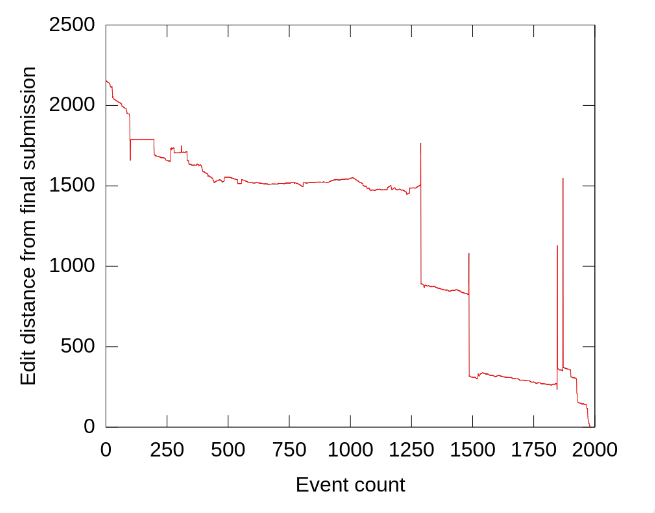
\includegraphics[scale=.25]{img/ed-a}
    \caption{Kasus A}\label{fig:edit-distance-a}
  \end{subfigure}%
  \begin{subfigure}{.5\linewidth}
    \centering
    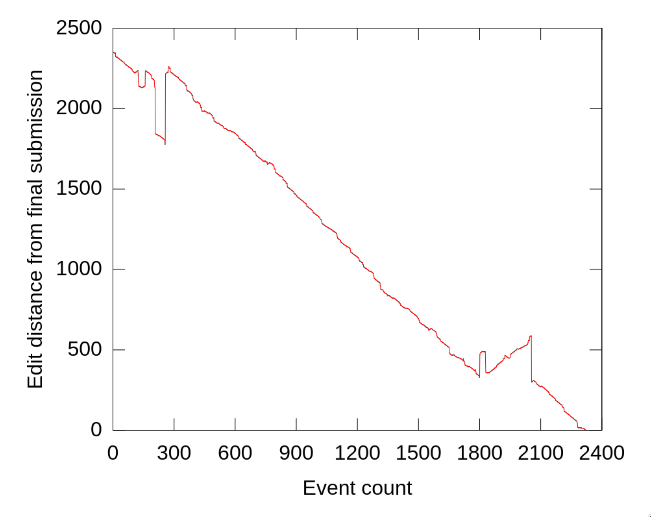
\includegraphics[scale=.25]{img/ed-b}
    \caption{Kasus B}\label{fig:edit-distance-b}
  \end{subfigure}\\[1ex]
  \begin{subfigure}{\linewidth}
    \centering
    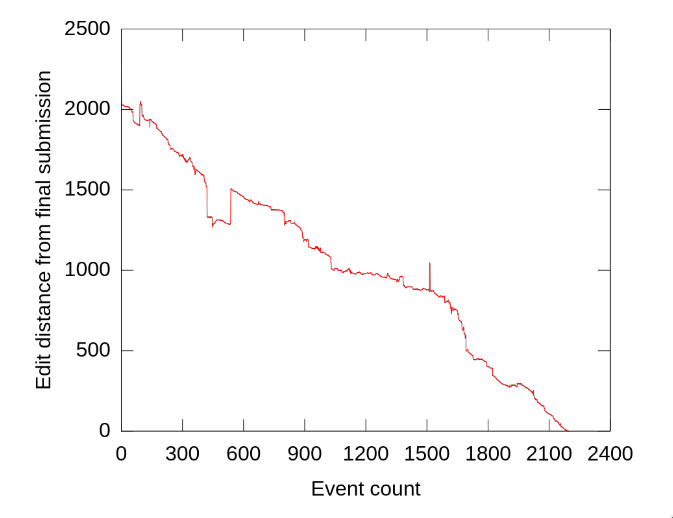
\includegraphics[scale=.25]{img/ed-c}
    \caption{Kasus C}\label{fig:edit-distance-c}
  \end{subfigure}
  \caption{Grafik \emph{edit-distance}}\label{fig:test}
\end{figure}

\section{Teknologi Pengembangan Perangkat Lunak}

\subsection{\emph{Python}}

\emph{Python} adalah bahasa pemrograman dengan \emph{syntax} yang elegan dan
sederhana yang dikembangkan oleh Guido van Rossum pada tahun 1990. \emph{Python}
bersifat \emph{interpreted} dan mendukung paradigma
\emph{object-oriented}. \emph{Python} juga memiliki dukungan struktur data
tingkat tinggi seperti \emph{dictionaries} dan \emph{list}. Berbeda dengan
bahasa \emph{scripting} yang lain, \emph{Python} dapat digunakan secara gratis,
bahkan untuk tujuan komersial \parencite{sanner1999python}.

\subsection{\emph{Git (Distributed Version Control)}}

\emph{Distributed version control} merupakan sebuah konsep di mana
aplikasi \emph{version control} dapat merekam semua perubahan yang
terjadi pada sebuah berkas secara terdistribusi atau tidak terpusat.
Sifatnya yang tidak terpusat memiliki kelebihan untuk melakukan semua
operasi secara lokal. Berbeda dengan \emph{version control} lainnya yang menggunakan \emph{diff}
untuk menyimpan berkas dari suatu waktu ke waktu, \emph{git} menggunakan
model \emph{snapshot} atau merekam seluruh berkas pada suatu waktu
tertentu. Hal ini memiliki kelebihan seperti kecepatan dalam
konstruksi berkas yang diminta pada waktu tertentu. Pada mulanya
\emph{git} dikembangkan oleh Linus Torvalds pada tahun 2005, Linus
kemudian menunjuk Junio Hamano untuk menjadi \emph{maintainer} hingga
sekarang \parencite{chacon2014pro}. \emph{Git} sejak awal diciptakan
secara modern sehingga memiliki integritas menggunakan \emph{hash}
\emph{SHA1} yang berupa 40 karakter heksadesimal. Hal ini yang
dijelaskan oleh Linus Torvalds sebagai \emph{content adressable}
layaknya \emph{filesystem} \parencite{gitmail1}. Tabel Kode~\ref{code:git-saved}
menunjukkan perintah pada \emph{git} untuk menyimpan perubahan suatu
berkas.

\par\null\par
\begin{code}
\begin{ignasicblock}[title=commit,minted language=text]
git commit -m "saved"
\end{ignasicblock}
  \captionof{listing}{Perintah untuk menyimpan perubahan pada
    \emph{git}}\label{code:git-saved}
\end{code}

\subsection{\emph{Qt (Widget Toolkit)}}

\emph{Qt} merupakan pustaka yang digunakan untuk membangun
\emph{graphical user interface}. Awalnya \emph{Qt} dikembangan oleh
Haavard Nord dan Eirik Chambe-Eng. Pada saat ini \emph{Qt}
dikembangan oleh \emph{The Qt Company} \parencite{qthistory}.
\emph{Qt} memiliki beberapa lisensi, di antaranya lisensi komersial dan
lisensi \emph{GPL 2.0}. Modul-modul yang dimiliki \emph{Qt} di antaranya adalah
\emph{Qt Core, Qt GUI,} dan \emph{Qt Widgets}
\parencite{qtabout}. Secara umum \emph{Qt} digunakan untuk
membangun \emph{graphical user interface} agar memudahkan interaksi
pengguna dengan aplikasi. Terlihat pada gambar~\ref{fig:hello-window} \emph{Qt} digunakan
untuk membuat \emph{window} sederhana dengan menggunakan kode pada
Tabel Kode~\ref{code:hello-window}.

\par\null\par
\begin{code}
\begin{ignasicblock}[title=hello,minted language=python]
import sys
from PyQt5.QtWidgets import QApplication, QWidget

if __name__ == '__main__':
    app = QApplication(sys.argv)
    window = QWidget()
    window.resize(250, 150)
    window.setWindowTitle('Hello World')
    window.show()
    sys.exit(app.exec_())
\end{ignasicblock}
  \captionof{listing}{Kode untuk membuat \emph{window} sederhana}\label{code:hello-window}
\end{code}

\begin{figure}[tph]
  \centering
  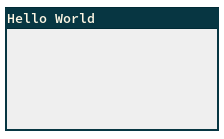
\includegraphics[width=.4\linewidth]{img/hello-window}
  \caption{\emph{Window} sederhana dengan \emph{Qt}}\label{fig:hello-window}
\end{figure}

\subsection{\emph{Draw.io}}

\emph{Draw.io} merupakan sebuah kakas bantu untuk menggambar
diagram ataupun \emph{mock up}. \emph{Draw.io} memiliki lisensi perangkat lunak bebas (\emph{Apache
  v2}) dan dapat diakses melalui peramban secara daring. \emph{Draw.io} dibangun
oleh Gaudenz Alder menggunakan bahasa pemrograman \emph{javascript} pada tahun 2000. Peramban
yang didukung diantaranya \emph{IE 11, Chrome 32+, Firefox 38+, Safari 9.1.x,}
dan \emph{Opera 20+} \parencite{drawio}.

%%% Local Variables:
%%% coding: utf-8
%%% mode: latex
%%% TeX-engine: xetex
%%% TeX-master: "skripsi"
%%% ispell-local-dictionary: "id"
%%% End:

%%%%%%%%%%%%%%%%%%%%%%%%%%%%%%%%%%%%%%%%%%%%%%%%%%%%%%%%%%%%%%%%%%%%%%%
% BAB 3
%%%%%%%%%%%%%%%%%%%%%%%%%%%%%%%%%%%%%%%%%%%%%%%%%%%%%%%%%%%%%%%%%%%%%%%

\mychapter{3}{BAB 3 METODOLOGI}

Pada bab ini akan dijelaskan langkah-langkah
penelitian. Langkah pertama diawali dengan studi literatur. Langkah selanjutnya
diikuti dengan rekayasa kebutuhan, perancangan, implementasi dan pengujian yang
merupakan urutan tahapan pada pengembangan sistem yang menggunakan model
\emph{waterfall}. Pemilihan model \emph{waterfall} dalam pengembangan sistem
pada penelitian ini disebabkan kebutuhan sistem yang sudah dapat didefinisikan
dengan baik pada tahap awal pengembangan sistem. Pengujian merupakan langkah
terakhir dalam pengembangan sistem pada penelitian ini, hal ini sesuai dengan
rumusan masalah penelitian. Langkah terakhir penelitian
ditutup dengan penarikan kesimpulan dan saran. Langkah-langkah tersebut dapat
dilihat pada pada Gambar~\ref{fig:diagram-alir}.

\begin{figure}[tph]
  \centering
  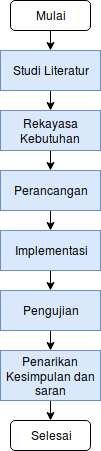
\includegraphics[width=.17\linewidth]{img/diagram-metodologi}
  \caption{Diagram alir metodologi}\label{fig:diagram-alir}
\end{figure}

\section{Studi Literatur}

Studi literatur dibutuhkan untuk mendalami teori-teori dan urgensi
tentang plagiarisme lebih dalam. Selain itu, studi literatur juga
dibutuhkan untuk mendalami teori rekayasa perangkat lunak untuk
mengembangkan perangkat lunak pencegah plagiarisme dengan menggunakan
metode \emph{snapshotting} dan \emph{user activity logging}. Sumber
dari literatur tersebut berasal dari jurnal, buku, situs resmi dan
dokumentasi perangkat lunak yang digunakan. Daftar literatur yang
dipelajari terkait dengan:

\begin{enumerate}
\item Penelitian-penelitian sebelumnya yang terkait dengan plagiarisme
\item Metode \emph{user activity logging, snapshotting} dan \emph{edit-distance algorithm}
\item Teori pengembangan perangkat lunak, yang di dalamnya meliputi
  teori rekayasa kebutuhan, perancangan, implementasi, dan pengujian
\item Teknologi yang digunakan dalam penelitian
\end{enumerate}

\section{Rekayasa Kebutuhan}

Rekayasa kebutuhan merupakan kumpulan tugas dan teknik untuk memahami
kebutuhan. Terdapat empat tahapan dalam rekayasa kebutuhan, yaitu
analisis kebutuhan, spesifikasi kebutuhan, manajemen kebutuhan, dan
pemodelan kebutuhan. Penjelasan tentang tahapan-tahapan yang dilakukan
dalam rekayasa kebutuhan adalah sebagai berikut:

\begin{enumerate}[
leftmargin=0pt, itemindent=20pt,
labelwidth=15pt, labelsep=5pt, listparindent=0.7cm,
align=left]

\item Analisis kebutuhan

  % - metode ihantola: waktu mulai + selesai, alamat IP
  % - kekurangan ihantola (``future work''') <- diperkuat oleh penelitian Leung: bantuan external
  % - sistem TMC Hellas yang platform dependend
  Pada tahapan ini dilakukan penggalian kebutuhan sistem. Kebutuhan fungsional
  sistem didapatkan dari:

  \begin{enumerate}
  \item Metode yang telah digunakan pada penelitian
    \parencite{hellas2017plagiarism}.
  \item ``\emph{Future work}'' penelitian \textcite{hellas2017plagiarism}, dan
    penelitian \textcite{leung2017instructional} yang memaparkan cara-cara
    plagiarisme di mana cara-cara tersebut belum dapat ditangani oleh penelitian
    \textcite{hellas2017plagiarism}.
  \item Kelemahan dari penelitian \textcite{hellas2017plagiarism} yang akan disempurnakan.
  \end{enumerate}

  Pada sumber kebutuhan fungsional pertama didapatkan kebutuhan fungsional untuk
  merekam waktu mulai pengerjaan, waktu selesai pengerjaan, rekaman alamat
  \emph{IP}, dan menghitung nilai \emph{edit-distance} pada berkas tugas.  Sumber
  kebutuhan fungsional kedua dan ketiga menghasilkan kebutuhan fungsional untuk
  merekam perubahan berkas tugas dengan metode \emph{snapshotting}, merekam
  aktivitas siswa menggunakan metode \emph{user activity logging}, dan
  mengembangkan sistem dengan sifat \emph{agnostic} agar tidak terikat pada
  \emph{platform} tertentu. Komponen aktivitas siswa yang direkam adalah seluruh
  \emph{window}, \emph{window} yang sedang aktif, nama \emph{login}, dan nama
  \emph{device}.

  Kebutuhan non-fungsional didapatkan dari batasan sistem yang hanya dapat
  berjalan pada sistem operasi \emph{GNU/Linux}, terdapat berbagai macam
  \emph{desktop environment} pada sistem operasi \emph{GNU/Linux} sehingga
  sistem yang dibangun harus \emph{compatible} dengan enam \emph{desktop
    environment} yang umum digunakan. Keenam \emph{desktop environment} tersebut
  adalah \emph{GNOME, KDE, XFCE, Unity, Cinnamon} dan \emph{Phanteon}.

\item Spesifikasi kebutuhan

  Pada tahapan ini hasil dari analisis kebutuhan pada tahapan
  sebelumnya dijelaskan secara lebih mendetail dengan jelas, tidak
  ambigu, mudah dipahami, dan konsisten. Kebutuhan fungsional
  mendeskripsikan apa yang dapat dilakukan oleh sistem yang dibangun
  dan kebutuhan non-fungsional mendeskripsikan batasan atau
  kualitas dari sistem yang dibangun.

\item Manajemen kebutuhan

  Tahapan ini dilakukan untuk memudahkan dalam mengidentifikasi, mengontrol
  dan melacak kebutuhan. Maka pada tahapan ini dilakukan
  kodefikasi pada kebutuhan-kebutuhan yang ada. Kode LUP-F-1 dan
  LUPR-F-1 untuk kebutuhan fungsional, LUPR-NF-1 dan LUPR-NR-1 untuk
  kebutuhan non-fungsional.

\item Pemodelan kebutuhan

  Tahap terakhir adalah pemodelan kebutuhan. Untuk menggambarkan fungsionalitas
  dan batasan sistem secara visual, penelitian ini menggunakan alat bantu
  \emph{use case diagram}, sedangkan untuk menjelaskan skenario interaksi antar aktor
  dan sistem secara mendetail, penelitian ini menggunakan alat bantu \emph{use
    case scenario}. Penggunaan kedua diagram tersebut dalam tahapan ini dapat
  memodelkan kebutuhan sistem baik secara visual (\emph{use case diagram})
  maupun secara tekstual dengan detail (\emph{use case scenario}).

\end{enumerate}

\section{Perancangan}

Tahapan perancangan sistem menjelaskan tentang rancangan sistem yang
akan dibangun berdasarkan hasil rekayasa kebutuhan pada tahapan
sebelumnya. Rancangan ini nantinya akan menjadi acuan pada tahap
implementasi dan pengujian. Tahap-tahap yang dilakukan pada perancangan
sistem adalah:

\begin{enumerate}[
leftmargin=0pt, itemindent=20pt,
labelwidth=15pt, labelsep=5pt, listparindent=0.7cm,
align=left]

\item Perancangan arsitektur

  Sistem akan dibangun dengan arsitektur \emph{Model-View-Controller}
  (\emph{MVC}). Arsitektur \emph{MVC} dipilih agar komponen fungsionalitas
  sistem terpisah dari komponen antarmuka sistem. Hal ini memudahkan
  pengembangan selanjutnya, karena pengembang
  cukup fokus pada masing-masing komponen yang terpisah. Arsitektur ini juga
  memudahkan proses \emph{porting} maupun penggantian antarmuka, karena
  pengembang cukup fokus pada komponen antarmuka sistem. Untuk menggambarkan
  interaksi yang terjadi antar komponen pada sistem, penelitian ini menggunakan
  alat bantu \emph{sequence digaram}. Terdapat tiga sampel \emph{sequence
    diagram} yang akan dipaparkan pada tahapan ini. Untuk menggambarkan struktur
  sistem dan relasi antar komponen pada sistem, penelitian ini menggunakan alat
  bantu \emph{class diagram}.

\item Perancangan komponen

  Pada tahapan ini komponen sistem akan dirancang menggunakan
  \emph{pseudocode}. \emph{Pseudocode} inilah yang nantinya menjadi
  acuan pada tahapan implementasi. Pada tahapan ini terdapat tiga
  sampel perancangan komponen yang akan dipaparkan.

\item Perancangan antarmuka

  Pada tahapan ini rancangan antarmuka sistem dan tata letak komponen antarmuka
  di dalamnya digambarkan dengan gambaran sederhana. Perancangan antarmuka
  dilakukan dengan kakas bantu \emph{draw.io}. Terdapat tiga
  sampel perancangan antarmuka yang akan dipaparkan pada tahapan ini.

\end{enumerate}

\section{Implementasi}

Pada tahapan implementasi, hasil perancangan pada tahapan sebelumnya
diimplementasikan, terdapat dua tahapan dalam implementasi yaitu:

\begin{enumerate}[
leftmargin=0pt, itemindent=20pt,
labelwidth=15pt, labelsep=5pt, listparindent=0.7cm,
align=left]

\item Implementasi kode program

  Pada tahapan ini hasil rancangan komponen sistem yang berupa \emph{pseudocode}
  diimplementasikan menjadi \emph{working code} menggunakan bahasa pemrograman
  \emph{Python}. Selain menggunakan \emph{Python}, metode \emph{snapshotting}
  yang diimplementasikan akan menggunakan bantuan kakas bantu \emph{git}.
\newpage % manual-adj
\item Implementasi antarmuka

  Pada tahapan ini hasil rancangan antarmuka sistem diimplementasikan
  menggunakan \emph{widget toolkit} \emph{Qt}.

\end{enumerate}

\section{Pengujian}

% NOTE
% - tahapan : unit, integration, validation
% - teknik: basis path, equivalence partitioning, bva
% - metode: black-box, white-box

Pada tahapan pengujian, dilakukan pengujian terhadap sistem yang telah
selesai diimplementasikan. Tahapan-tahapan yang akan dilakukan adalah:

\begin{enumerate}[
leftmargin=0pt, itemindent=20pt,
labelwidth=15pt, labelsep=5pt, listparindent=0.7cm,
align=left]

\item Pengujian unit

  % untuk memastikan rancangan komponen! Makanya di uji ke pseuodcode
  Tahap pengujian unit dilakukan untuk memastikan hasil implementasi kode
  program sesuai dengan hasil perancangan komponen. Penelitian ini mengikuti
  pendapat \textcite{pressman2010software} terkait dengan pemahaman
  \emph{unit}. Maka tahapan ini menguji setiap unit terkecil dari sistem yaitu
  sebuah \emph{class}. \emph{Class} \emph{controller} dan \emph{model} diuji hingga
  batas \emph{code coverage} mencapai 100\%, karena semua kode inti program terdapat
  pada kedua \emph{class} tersebut. Berbeda dengan \emph{class} \emph{view} hanya
  memanggil fungsi-fungsi yang terdapat pada \emph{class} \emph{controller} dan
  \emph{model} sehingga pada penelitian ini pengujian unit pada \emph{class}
  \emph{view} hanya diuji hingga \emph{code coverage} mencapai 70\%. Pengujian unit
  dilakukan menggunakan metode \emph{white-box testing} dan kasus uji didapatkan
  dengan teknik \emph{basis path testing}. Pengujian setiap unit pada tahapan
  ini dilakukan secara terisolasi sehingga dilakukan pembuatan \emph{stub} atau
  ``\emph{dummy subprogram}''. Terdapat tiga sampel pengujian unit yang akan
  dipaparkan pada tahapan ini.

\item Pengujian integrasi

  % untuk mengecek integrasi antar unit
  Setelah semua unit selesai diuji, maka dilakukan tahapan pengujian
  integrasi. Pengujian integrasi dilakukan untuk memastikan integrasi antar unit
  berjalan dengan baik. Maka pada pengujian integrasi, \emph{function} pada
  suatu \emph{class} yang memanggil \emph{function} pada \emph{class} lain tidak
  digantikan dengan \emph{stub} atau \emph{fake} sebagaimana ketika pada
  pengujian unit. Pada penelitian ini perangkat lunak yang dikembangkan
  menggunakan pendekatan dan pengembangan berorientasi objek sehingga pendekatan pengujian
  integrasi yang digunakan adalah \emph{use-based testing}. Integrasi
  diawali dari \emph{class} yang memiliki \emph{dependent class} paling
  sedikit, yaitu dimulai dari \emph{class} \emph{model}, kemudian
  \emph{class controller}, dan yang terakhir adalah \emph{class}
  \emph{view}. Pengujian integrasi menggunakan metode \emph{white-box
    testing} dan teknik \emph{basis path testing}. Terdapat satu
  sampel yang dipaparkan pada tahapan ini.
\newpage % manual-adj
\item Pengujian validasi

  % kurang lebih sama seperti acceptance testing, ngecek apakah sudah sesuai
  % dengan spesifikasi kebutuhan
  % hanya fokus pada user visible/ not internal
  Pengujian validasi menguji apakah sistem yang dibangun sudah sesuai dengan
  kebutuhan yang didefinisikan. Pengujian validasi fokus terhadap
  \emph{user-visible action} dan \emph{user-recognizable output} dari sistem
  \parencite{pressman2010software}. Maka pada tahapan ini seluruh skenario
  kebutuhan diuji. Pengujian validasi dilakukan menggunakan metode
  \emph{black-box testing}. Teknik yang digunakan untuk mendapatkan kasus uji
  dan data uji adalah teknik \emph{equivalence partitioning} dan \emph{boundary
    value analysis}. Kedua teknik tersebut digunakan untuk menghindari
  \emph{rigorous testing} atau mencoba semua kemungkinan.

\item \emph{Automated testing}

  % terjamah kasus uji pada unit & integrasi jadi script!, kemudian di
  % jalankan secara otomatis
  \emph{Automated testing} dilakukan untuk meminimalisir waktu yang digunakan
  untuk pengujian. Pada tahapan ini dibangun \emph{script} yang menjalankan
  kasus uji secara otomatis. Kasus uji didapatkan dari pengujian unit dan
  pengujian integrasi yang telah dilakukan pada tahapan
  sebelumnya. \emph{Automated testing} berjalan secara otomatis jika terjadi
  perubahan pada berkas \emph{source code} sistem. Penelitian ini menggunakan
  kakas bantu \emph{Pytest} untuk membangun \emph{script}, dan menggunakan
  \emph{Gitlab-CI} untuk menjalankan \emph{script} secara otomatis. Terdapat
  tiga sampel \emph{automated testing} yang dipaparkan pada tahapan ini.

\item Pengujian \emph{compatibility}

  % setiap de window itu beda
  Pengujian \emph{compatibility} merupakan pengujian terhadap
  kebutuhan non-fungsional sistem. Pada pengujian
  ini sistem \emph{Lup Recorder} dan \emph{Lup Viewer} dijalankan pada
  enam \emph{desktop environment} yang umum digunakan pada sistem
  operasi \emph{GNU/Linux}. Keenam \emph{desktop environment} tersebut
  adalah \emph{GNOME, KDE, XFCE, Unity, Cinnamon} dan \emph{Phanteon}.
  Pengujian ini dilakukan untuk memastikan apakah sistem
  yang dibangun sudah \emph{compatible} dengan berbagai macam
  \emph{desktop environment}.

\end{enumerate}

\section{Penarikan Kesimpulan}

Kesimpulan akan ditarik pada akhir penelitian. Penarikan kesimpulan dapat
dilakukan setelah tahap analisis kebutuhan, perancangan, implementasi, dan
pengujian selesai dilakukan. Kesimpulan akan ditarik berdasarkan dari analisis
hasil sistem yang telah dibangun. Kesimpulan tersebut akan menjawab rumusan
masalah yang telah dipaparkan dan memuat catatan untuk pengembangan sistem di
waktu mendatang.


%%% Local Variables:
%%% coding: utf-8
%%% mode: latex
%%% TeX-engine: xetex
%%% TeX-master: "skripsi"
%%% ispell-local-dictionary: "id"
%%% End:

%%%%%%%%%%%%%%%%%%%%%%%%%%%%%%%%%%%%%%%%%%%%%%%%%%%%%%%%%%%%%%%%%%%%%%%
% BAB 4
%%%%%%%%%%%%%%%%%%%%%%%%%%%%%%%%%%%%%%%%%%%%%%%%%%%%%%%%%%%%%%%%%%%%%%%

\mychapter{4}{BAB 4 METODOLOGI}

Bab ini menjelaskan tentang langkah-langkah yang dilakukan selama
pengembangan pengujian. Setelah studi literatur selesai dilakukan,
dilaksanakan proses analisis kebutuhan pengujian, perencanaan dan
implementasi kasus uji, dan penarikan kesimpulan.

\begin{figure}[H]
  \centering
  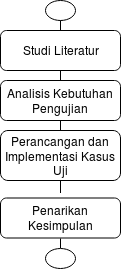
\includegraphics[width=.2\linewidth]{img/diagram-uji3}
  \caption{Alur metodologi}
  \label{fig:alur-metodologi}
\end{figure}

\section{Studi Literatur}

Studi Literatur dibutuhkan untuk mendalami teori-teori tentang
pengujian lebih dalam. Sumber dari literatur tersebut berasal dari
jurnal, buku, situs resmi maupun buku panduan perangkat lunak
yang digunakan. Daftar literatur yang didalami terkait dengan:

\begin{enumerate}
\item Penelitian-penelitian terkait pengujian
\item Metode-metode pengujian yaitu \emph{white-box} dan \emph{black-box}.
\item Tahapan pengujian \emph{unit} dan \emph{integration}.
\item Teknik pengujian \emph{basis path testing, boundary value
    analysis} dan \emph{ equivalence partitioning}.
\item Teknologi yang digunakan dalam penelitian
\end{enumerate}

\section{Analisis Kebutuhan Pengujian}

Pada proses analis kebutuhan pengujian akan ditentukan tahapan yang
akan di lakukan dan bagian yang akan diuji. Pengujian pada
\emph{neo-cli} hanya dilakukan hanya pada tahapan \emph{unit} dan
\emph{integration}.  Pada fase ini ditentukan juga \emph{method}
apa saja yang akan diuji. Penentuan tahapan pengujian dan penetuan
\emph{method} yang akan diuji dilakukan oleh pembimbing lapangan
dengan beberapa pertimbangan. Di antara pertimbangan tersebut adalah
waktu praktik kerja lapangan yang terbatas.

\section{Perancangan dan Implementasi Kasus Uji}

Pada proses ini dilakukan perancangan dan implementasi (eksekusi)
kasus uji. Tahapan yang dilakukan diawali dengan pengujian \emph{unit}
kemudian pengujian \emph{integration}. Metode pengujian yang digunakan
adalah metode pengujian \emph{white-box} dan metode pengujian
\emph{black-box}. Teknik yang digunakan selama proses pengujian dengan
methode \emph{white-box} adalah teknik \emph{basis path testing}.
Teknik \emph{equivalence partitioning} dan \emph{boundary value
  analysis} adalah teknik yang digunakan selama proses pengujian
dengan metode \emph{black-box}. Perancangan kasus uji dalam metode
\emph{white-box} diawali dengan pembuatan \emph{flow graph} dari
sebuah \emph{pseudocode}, kemudian menghitung \emph{cyclomatic
  complexity}, menentukan \emph{independent path} dan merancang kasus
uji sesuai dengan \emph{idependent path} yang didapatkan. Sedangkan
perancangan kasus uji pada metode \emph{black-box} didapatkan dari
data pengujian yang dihasilkan dari penggunaan teknik
\emph{equivalence partitioning} dan \emph{boundary value analysis}.
Implementasi pengujian atau eksekusi pengujian dilakukan secara
langsung setelah perancangan pada tahapan \emph{unit} dan
\emph{integration} selesai. Hasil dari implementasi tersebut juga
langsung dipaparkan. Hasil dari implementasi atau eksekusi pengujian
diletakkan pada kolom \emph{result} dan \emph{status} pada tabel kasus
uji. Metode pengujian \emph{white-box} dilakukan pada seluruh tahapan
\emph{unit} dan \emph{integration}. Sedangkan metode pengujian
\emph{black-box} hanya dilakukan pada bagian integrasi sistem yang
meminta masukan kepada pengguna, seperti yang terjadi pada
\emph{method do\_login}. Setelah pengujian secara manual pada tahap
\emph{unit} dan \emph{integration} selesai dilakukan, maka dibangun
\emph{test script} untuk \emph{automated testing} sehingga proses
pengujian selanjutnya dapat dilakukan secara otomatis. \emph{Automated
  testing} dilakukan menggunakan bantuan kakas bantu \emph{travis-ci}
yang konfigurasinya dijelaskan pada subbab ``Pengaturan Lingkungan
Pengujian untuk \emph{Automated Testing}''. Perhitungan cakupan
pengujian dilakukan dengan bantuan kakas bantu \emph{coverage.py} yang
hasil cakupannya dijelaskan pada subbab ``Hasil Cakupan Pengujian''.

\section{Penarikan Kesimpulan}

Pengujian ditutup setelah semua \emph{method} pada analisis kebutuhan
pengujian selesai diuji. Penarikan kesimpulan dilakukan setelah
pengujian ditutup. Kesimpulan diambil berdasarkan hasil dari seluruh
proses yang dilakukan selama pengujian. Kesalahan-kesalahan akan dicat
dan dijadikan saran agar tidak terulang kembali pada proses pengujian
selanjutnya. Kesimpulan pengujian nantinya dapat digunakan untuk
perbaikan dan peningkatan pengujian-pengujian selanjutnya.

%%% Local Variables:
%%% mode: latex
%%% TeX-master: "pkl"
%%% End:

%%%%%%%%%%%%%%%%%%%%%%%%%%%%%%%%%%%%%%%%%%%%%%%%%%%%%%%%%%%%%%%%%%%%%%%
% BAB 5
%%%%%%%%%%%%%%%%%%%%%%%%%%%%%%%%%%%%%%%%%%%%%%%%%%%%%%%%%%%%%%%%%%%%%%%

\mychapter{5}{BAB 5 PERANCANGAN DAN IMPLEMENTASI}

\section{Perancangan Sistem}

Tahapan perancangan sistem merupakan sebuah tahapan yang dilakukan
setelah selesainya proses rekayasa kebutuhan. Hasil tahapan
perancangan nantinya digunakan sebagai landasan tahapan implementasi
sistem. Tiga bagian yang terdapat pada tahapan ini adalah
perancangan arsitektur, perancangan komponen, dan perancangan
antarmuka.

\subsection{Perancangan Arsitektur}

Sistem dibangun menggunakan arsitektur \emph{Model-View-Controller (MVC)}.
Maka komponen fungsionalitas inti sistem terpisah dari komponen antarmuka
sistem. Pemisahan ini memberikan manfaat untuk pengembangan sistem pada tahap
selanjutnya. Salah satu manfaat tersebut adalah kemudahan dalam mengembangkan
antarmuka lain untuk sistem, hal ini dikarenakan pengembang hanya fokus pada
komponen antarmuka yang akan dibangun.
Perancangan arsitektur dilakukan dengan menggunakan notasi \emph{UML}
\emph{sequence diagram} dan \emph{class diagram}. \emph{Class diagram}
bertujuan menggambarkan struktur sistem dan relasi antar komponen dalam sistem
secara statis. Pada \emph{class diagram} digambarkan \emph{class},
\emph{method} atau
\emph{function}, dan relasi antar \emph{class}. \emph{Sequence
  diagram} merupakan diagram dinamis yang berfungsi untuk
menggambarkan interaksi antar komponen atau objek yang berada di dalam sistem.
Terdapat tiga sampel \emph{sequence diagram} yang akan dipaparkan pada
bagian ini. Tiga sampel tersebut adalah \emph{sequence diagram} untuk
merekam pengerjaan tugas, \emph{sequence diagram} untuk melihat hasil
rekaman, dan \emph{sequence diagram} untuk melihat grafik \emph{edit-distance}
tugas sebelumnya. Sementara itu, \emph{class diagram} sistem akan dipaparkan seluruhnya.

\subsubsection{\emph{Sequence Diagram} Merekam Pengerjaan Tugas}

\emph{Sequence diagram} untuk merekam pengerjaan tugas dapat
dilihat pada Gambar~\ref{fig:sd-record}. Pada \emph{sequence diagram}
tersebut terdapat beberapa objek yang berinteraksi. Satu objek
\emph{boundary} ``\emph{MainView}'', dua objek \emph{controller}
``\emph{Controller}'' dan ``\emph{RecordWorker}'', dan satu objek
\emph{entity} ``\emph{Model}''. Aktor yang terlibat adalah mahasiswa.

\subsubsection{\emph{Sequence Diagram} Melihat Hasil Rekaman}

\emph{Sequence diagram} untuk melihat hasil rekaman dapat
dilihat pada Gambar~\ref{fig:sd-view-record-result}. Pada \emph{sequence diagram}
tersebut terdapat beberapa objek yang berinteraksi. Dua objek
\emph{boundary} ``\emph{MainView}'' dan ``\emph{LogView}'', dua objek \emph{controller}
``\emph{LogController}'' dan ``\emph{MainController}'', dan satu objek
\emph{entity} ``\emph{LogModel}''. Aktor yang terlibat adalah dosen.

\subsubsection{\emph{Sequence Diagram} Melihat Grafik \emph{Edit-Distance} Tugas Sebelumnya}

\emph{Sequence diagram} untuk melihat grafik \emph{edit-distance} tugas
sebelumnya dapat dilihat pada Gambar~\ref{fig:sd-view-previous-ed}.
Pada \emph{sequence diagram} tersebut terdapat beberapa objek yang
berinteraksi. Satu objek \emph{boundary} ``\emph{SearchView}'', satu objek
\emph{controller} ``\emph{SearchController}'', dan dua objek \emph{entity}
``\emph{SearchModel}'' dan ``\emph{MainModel}''. Aktor yang terlibat adalah dosen.

\begin{figure}[tph]
  \centering
  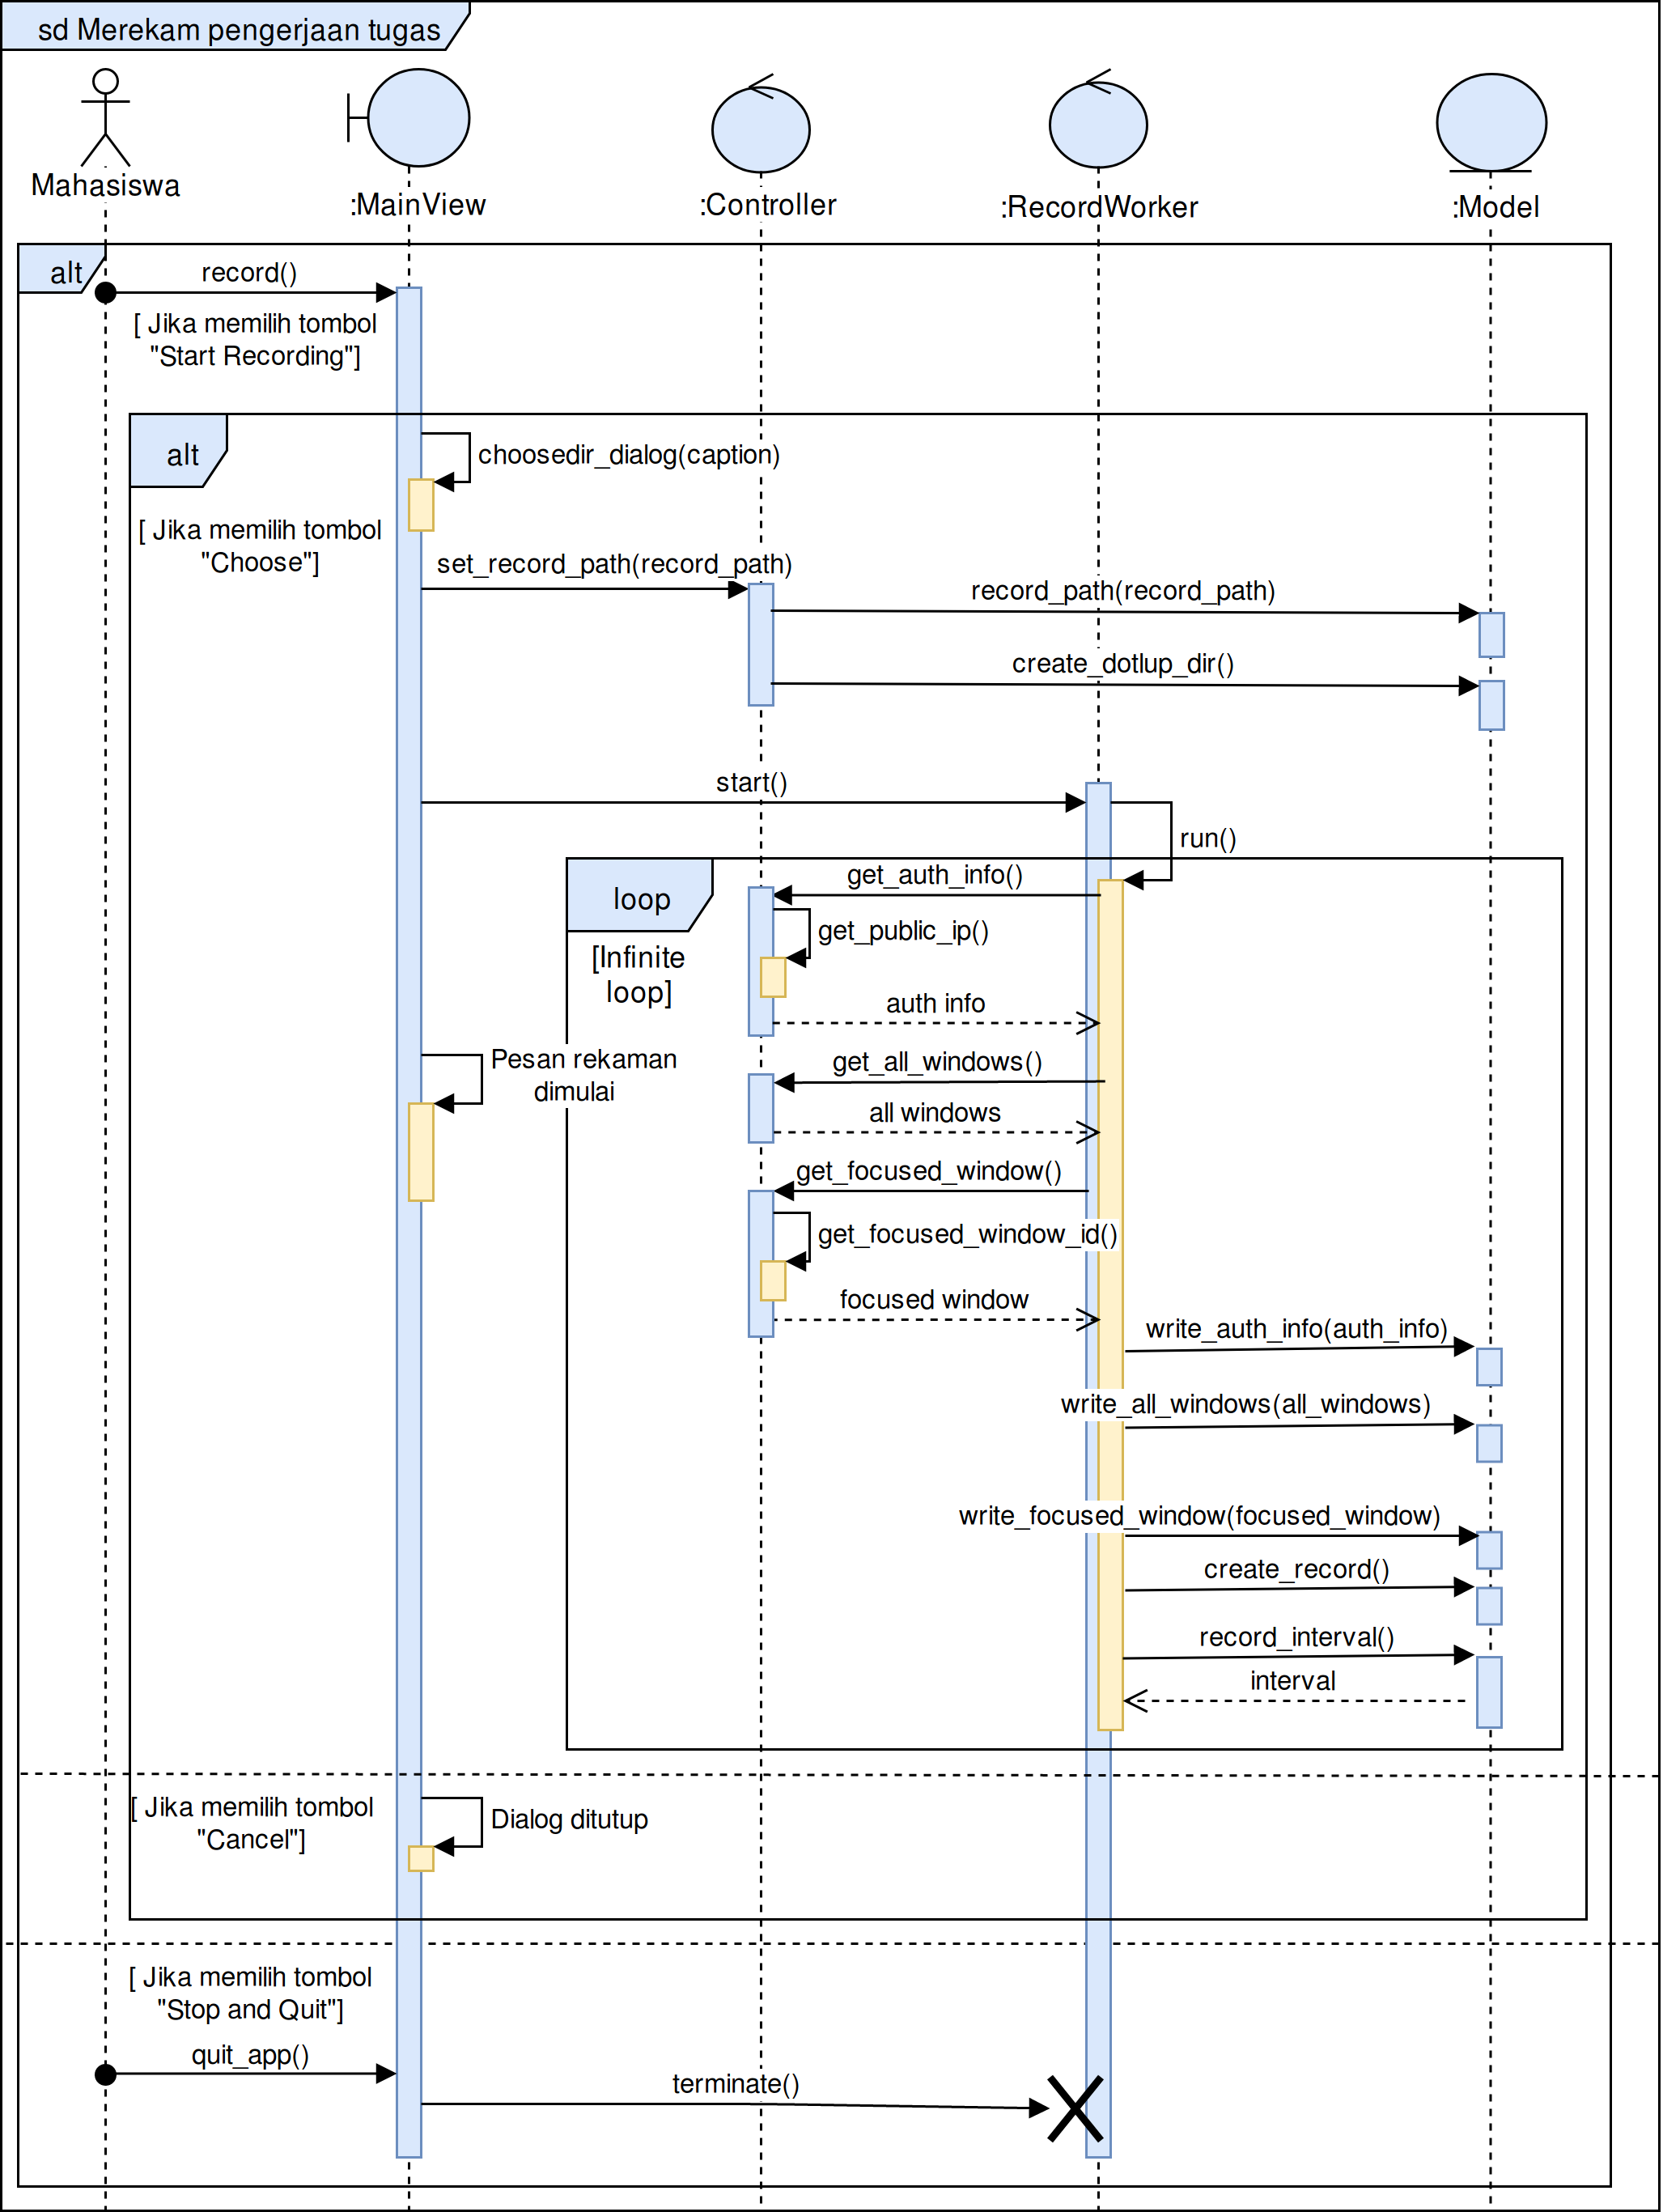
\includegraphics[width=.9\linewidth]{img/use-case/sd/sd-record-v2_4}
  \caption{\emph{Sequence diagram} Merekam Pengerjaan Tugas}\label{fig:sd-record}
\end{figure}

\begin{figure}[tph]
  \centering
  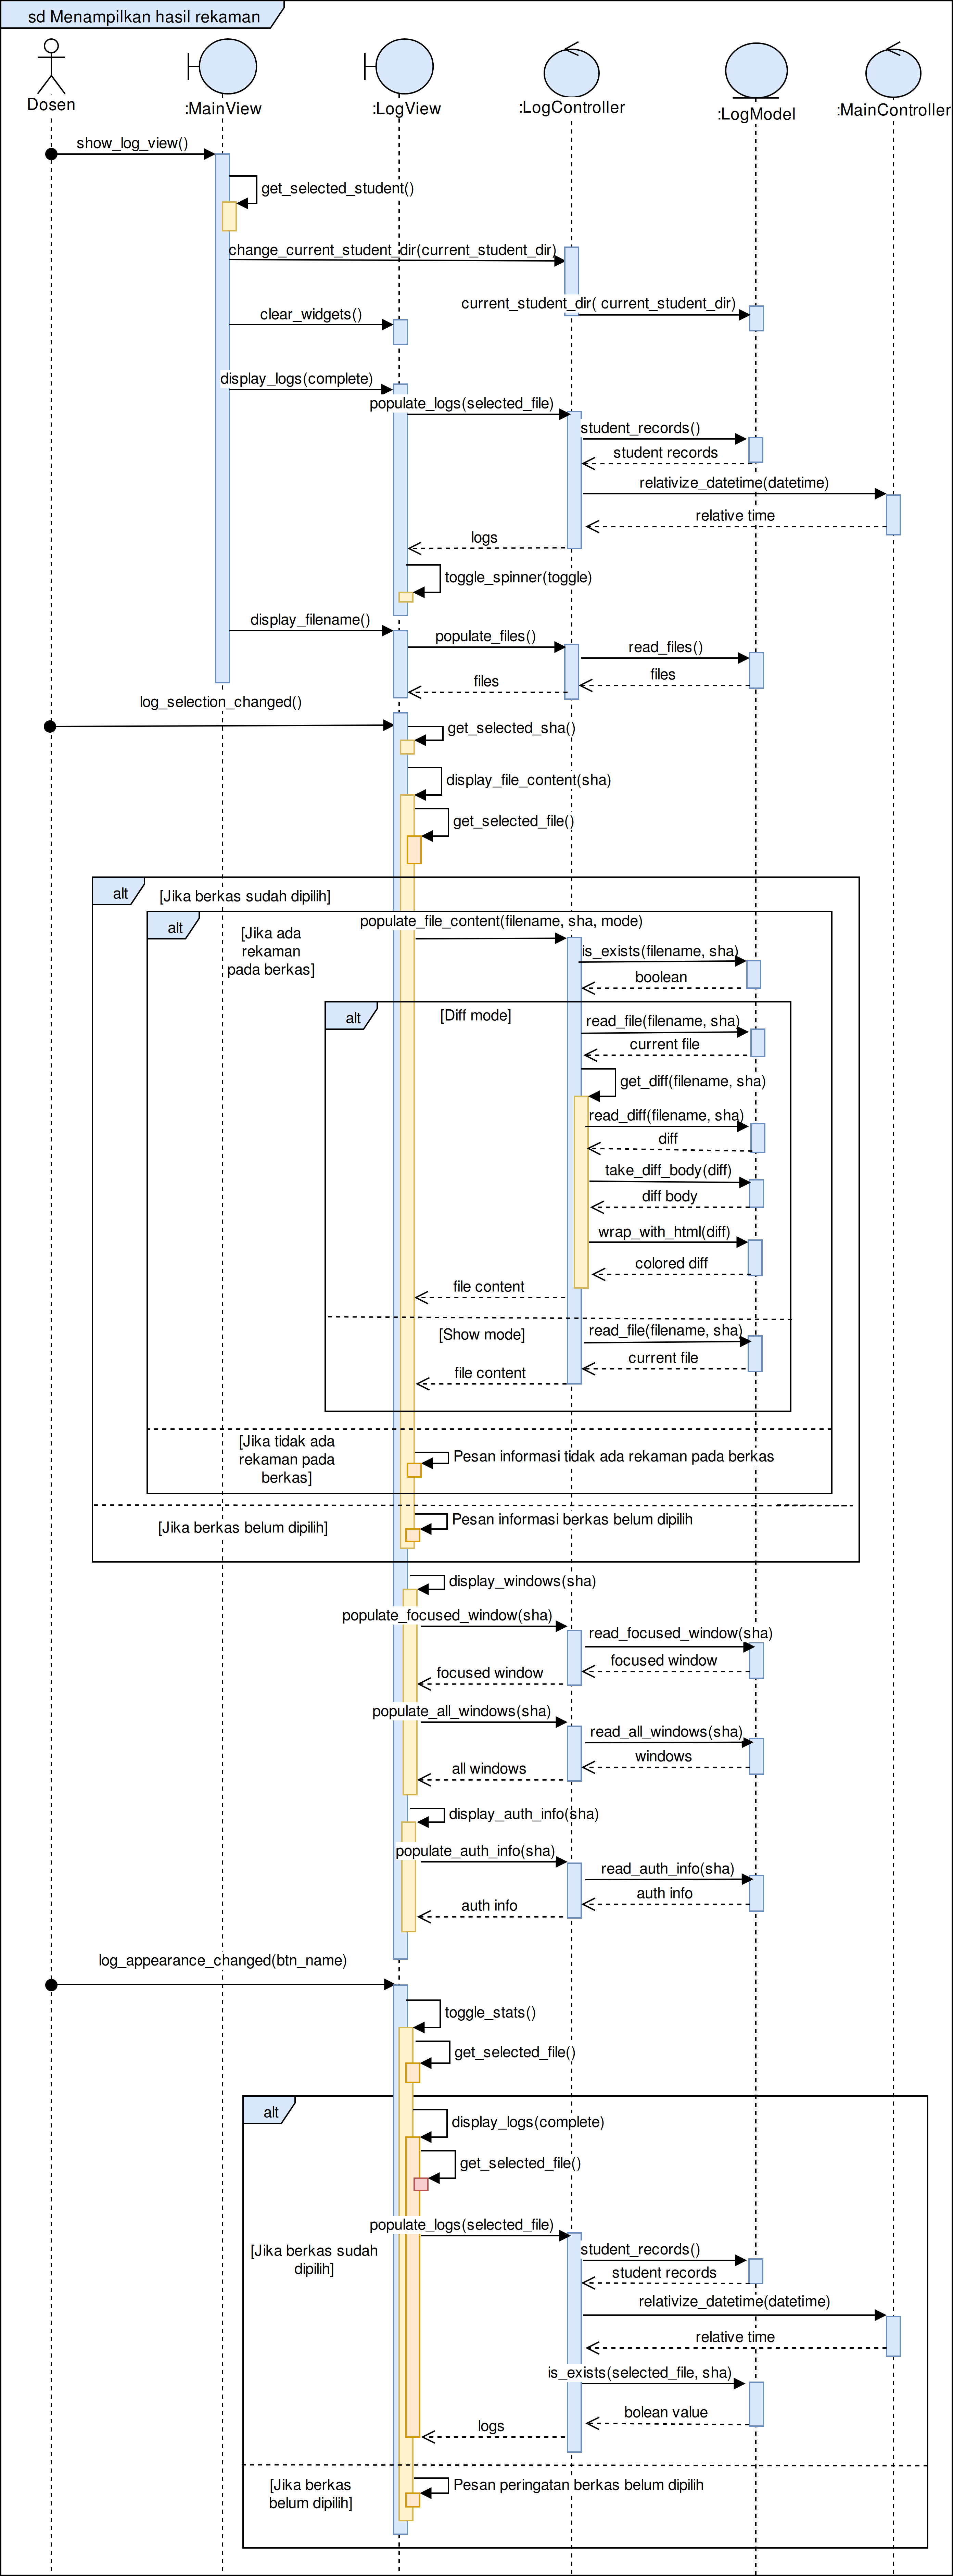
\includegraphics[width=.6\linewidth]{img/use-case/sd/sd-view-record-result-v1}
  \caption{\emph{Sequence diagram} Melihat Hasil Rekaman}\label{fig:sd-view-record-result}
\end{figure}

\begin{figure}[tph]
  \centering
  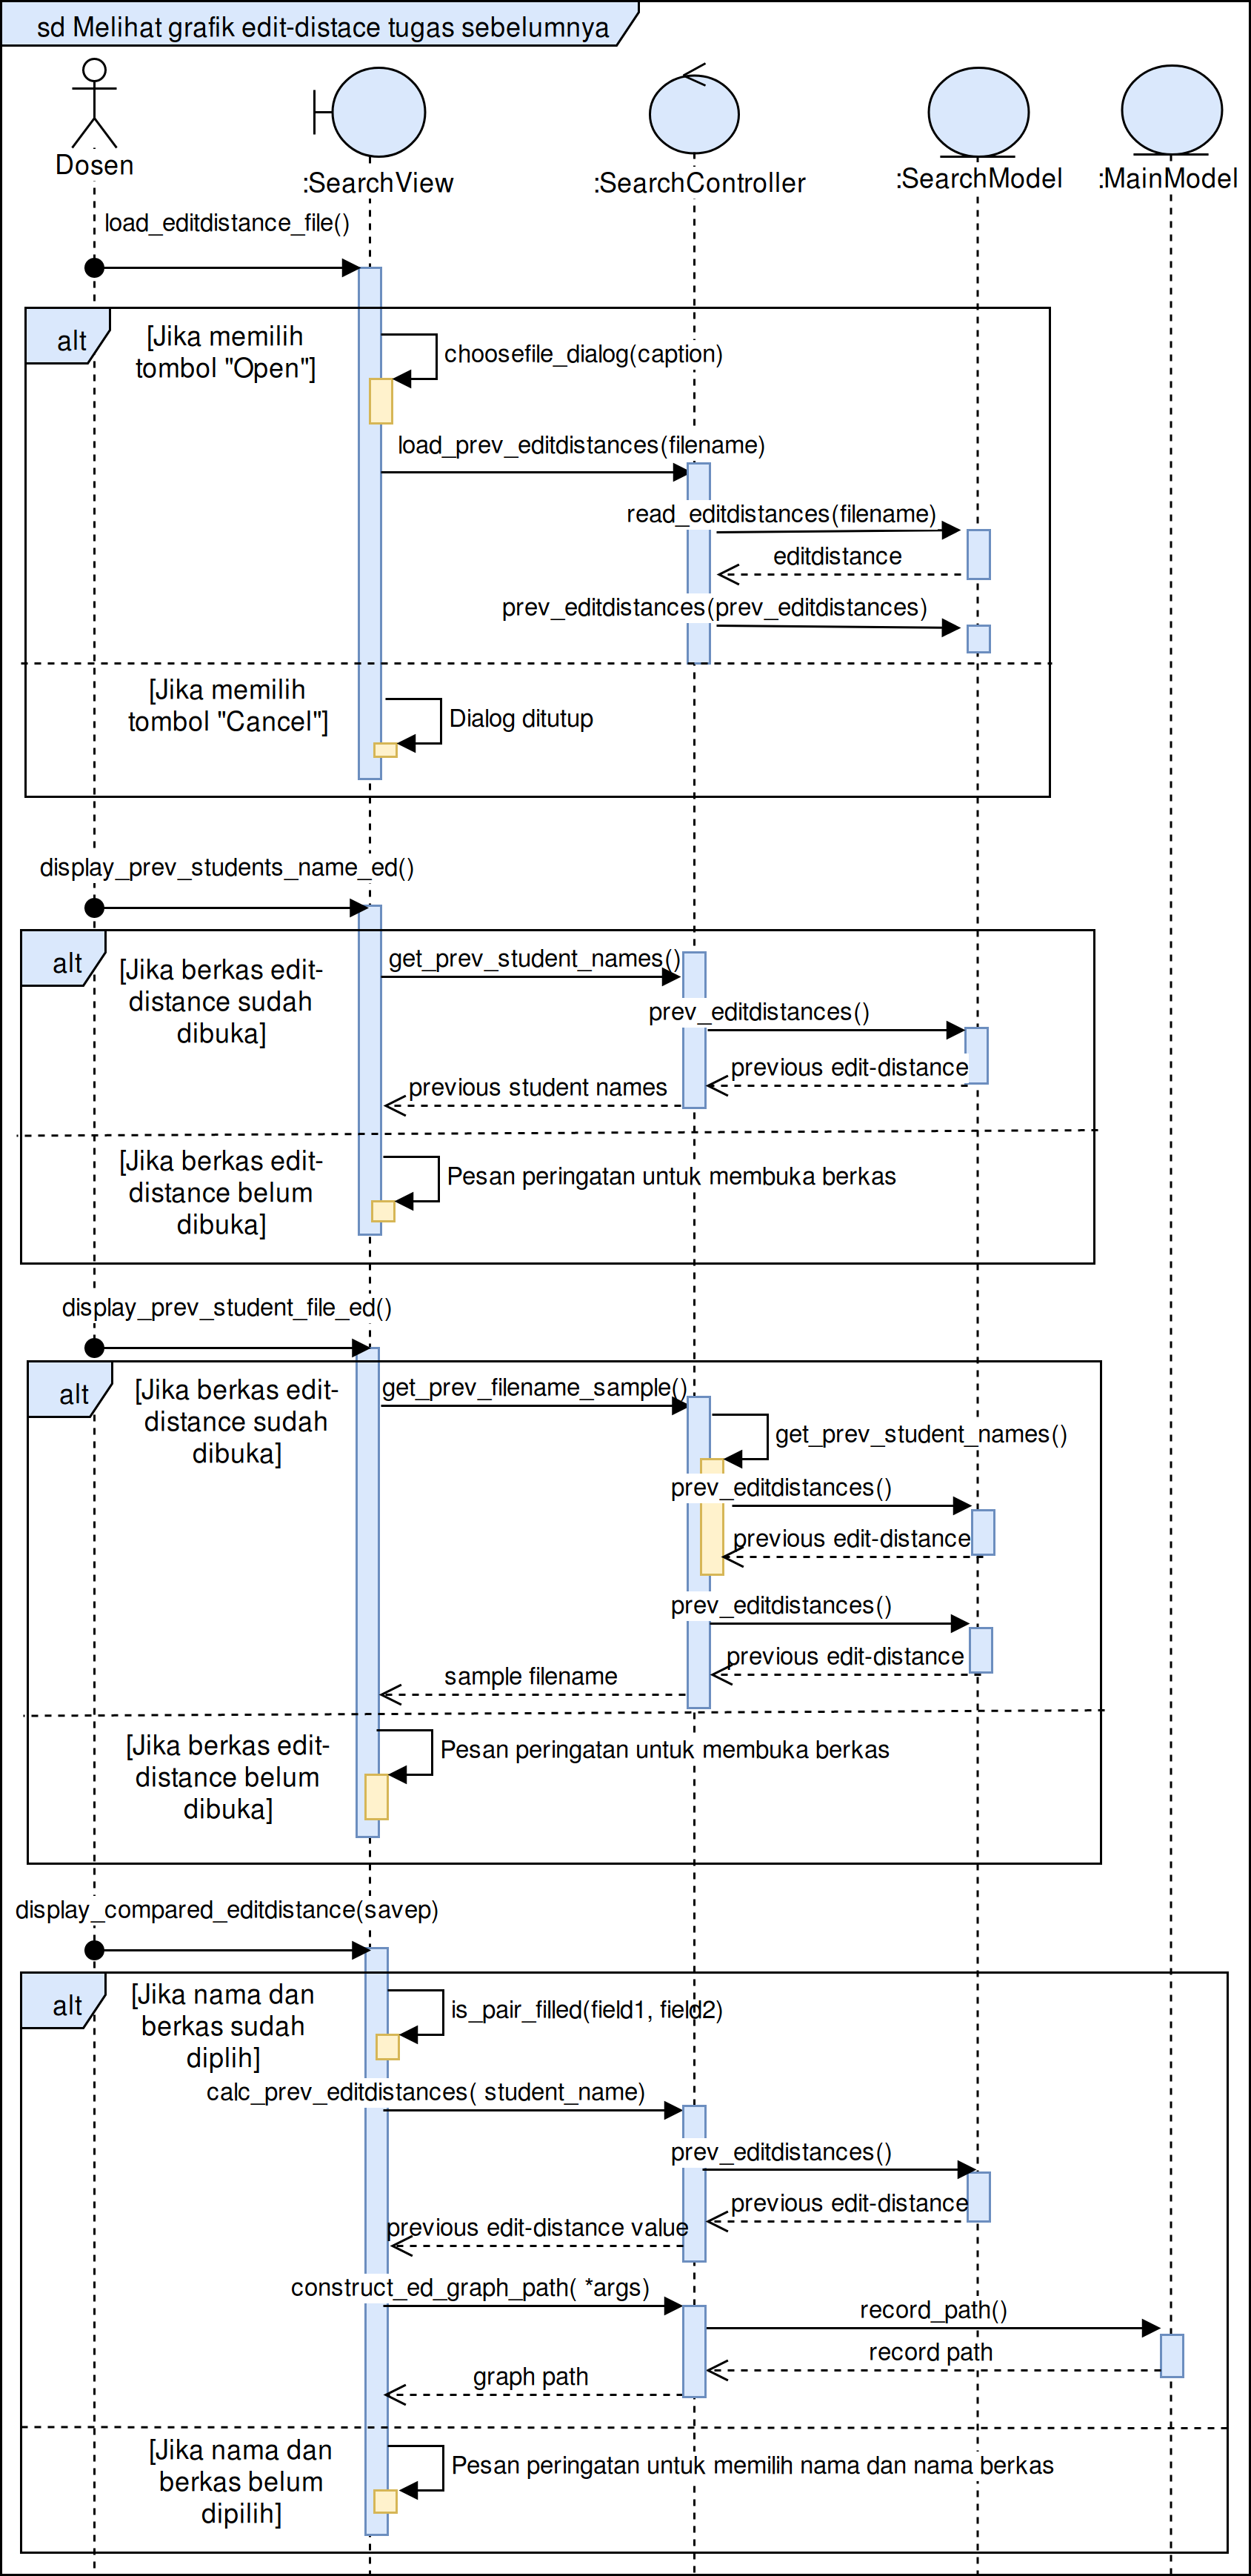
\includegraphics[width=.8\linewidth]{img/use-case/sd/sd-view-previous-ed-v1_2}
  \caption{\emph{Sequence diagram} Melihat Grafik \emph{Edit-Distance} Tugas
    Sebelumnya}\label{fig:sd-view-previous-ed}
\end{figure}

\subsubsection{\emph{Class Diagram}}

Pada bagian ini akan dipaparkan \emph{class}-\emph{class} yang menyusun sistem yang
dibangun. Gambar~\ref{fig:class-lupr} merupakan \emph{class diagram}
dari sistem \emph{Lup Recorder}, dan Gambar~\ref{fig:class-lupv}
merupakan \emph{class diagram} dari sistem \emph{Lup Viewer}. Sistem
yang dibangun menggunakan arsitektur \emph{Model-View-Controller}
sehingga \emph{class}-\emph{class} yang menyusun sistem pada \emph{class diagram}
umumnya terdiri dari \emph{class} \emph{Model}, \emph{class} \emph{View} dan \emph{class}
\emph{Controller}. Pada \emph{class diagram} juga dipaparkan relasi
antar \emph{class} yang umumnya merupakan relasi agregasi dan komposisi.

\begin{figure}[tph]
  \centering
  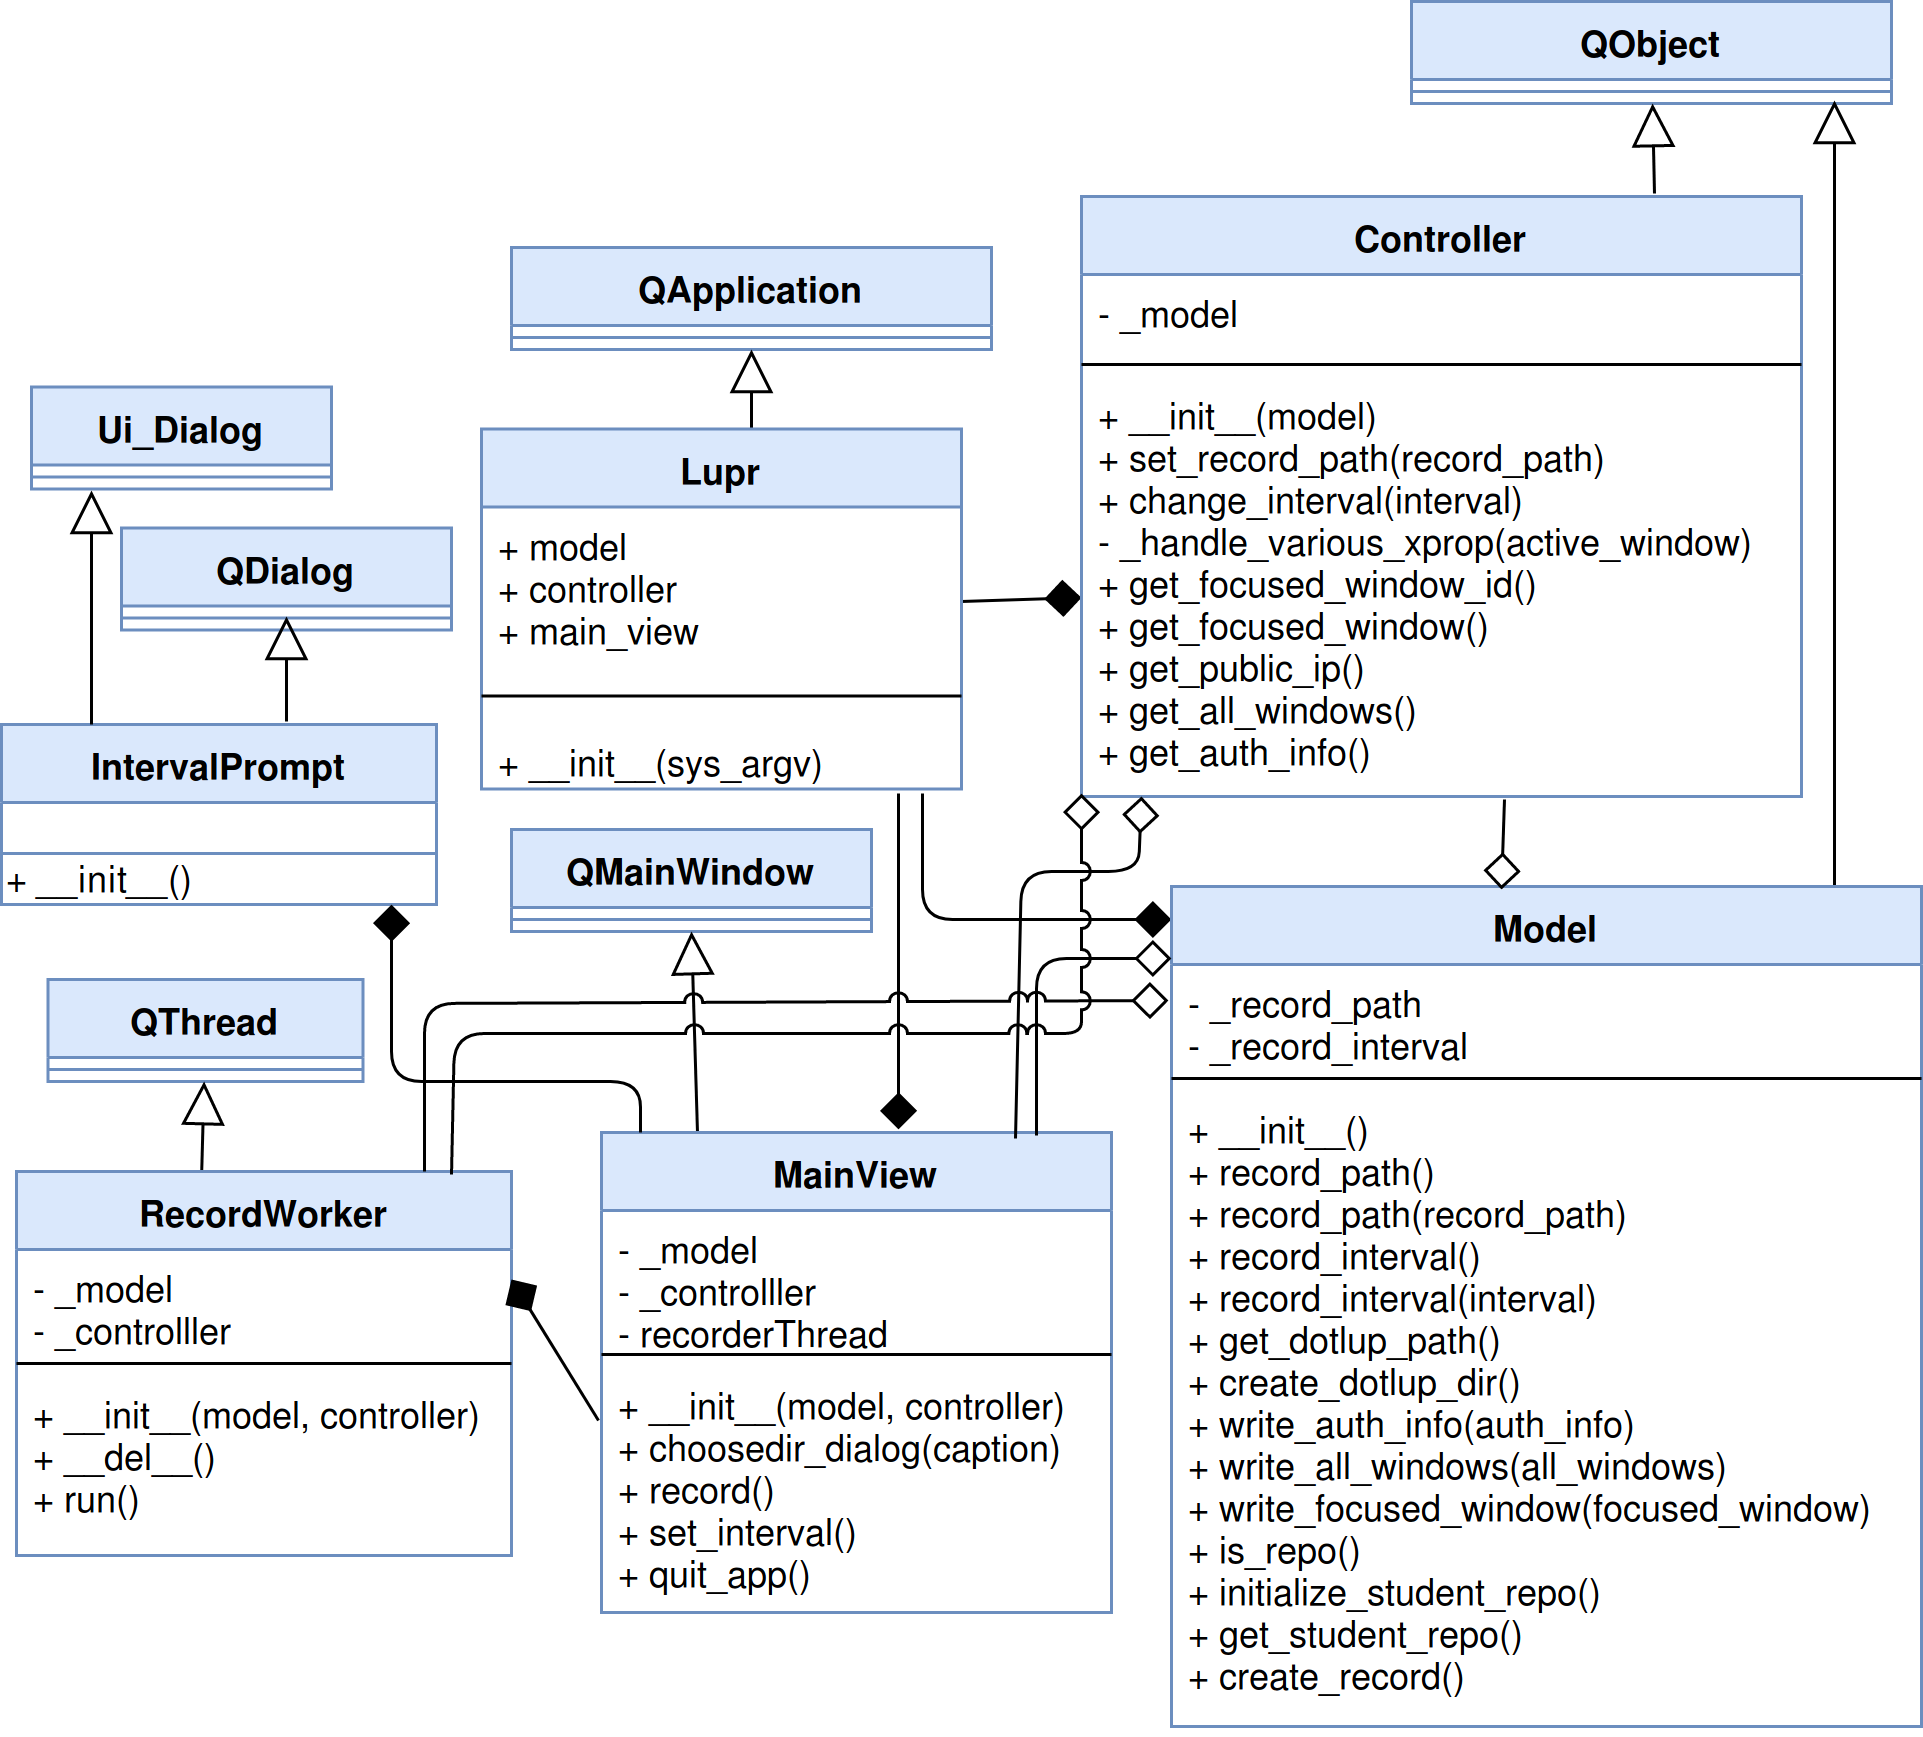
\includegraphics[width=.9\linewidth]{img/use-case/cd/class-lupr-v1_4}
  \caption{Pemodelan \emph{class diagram} \emph{Lup Recorder}}\label{fig:class-lupr}
\end{figure}

\begin{figure}[tph]
  \centering
  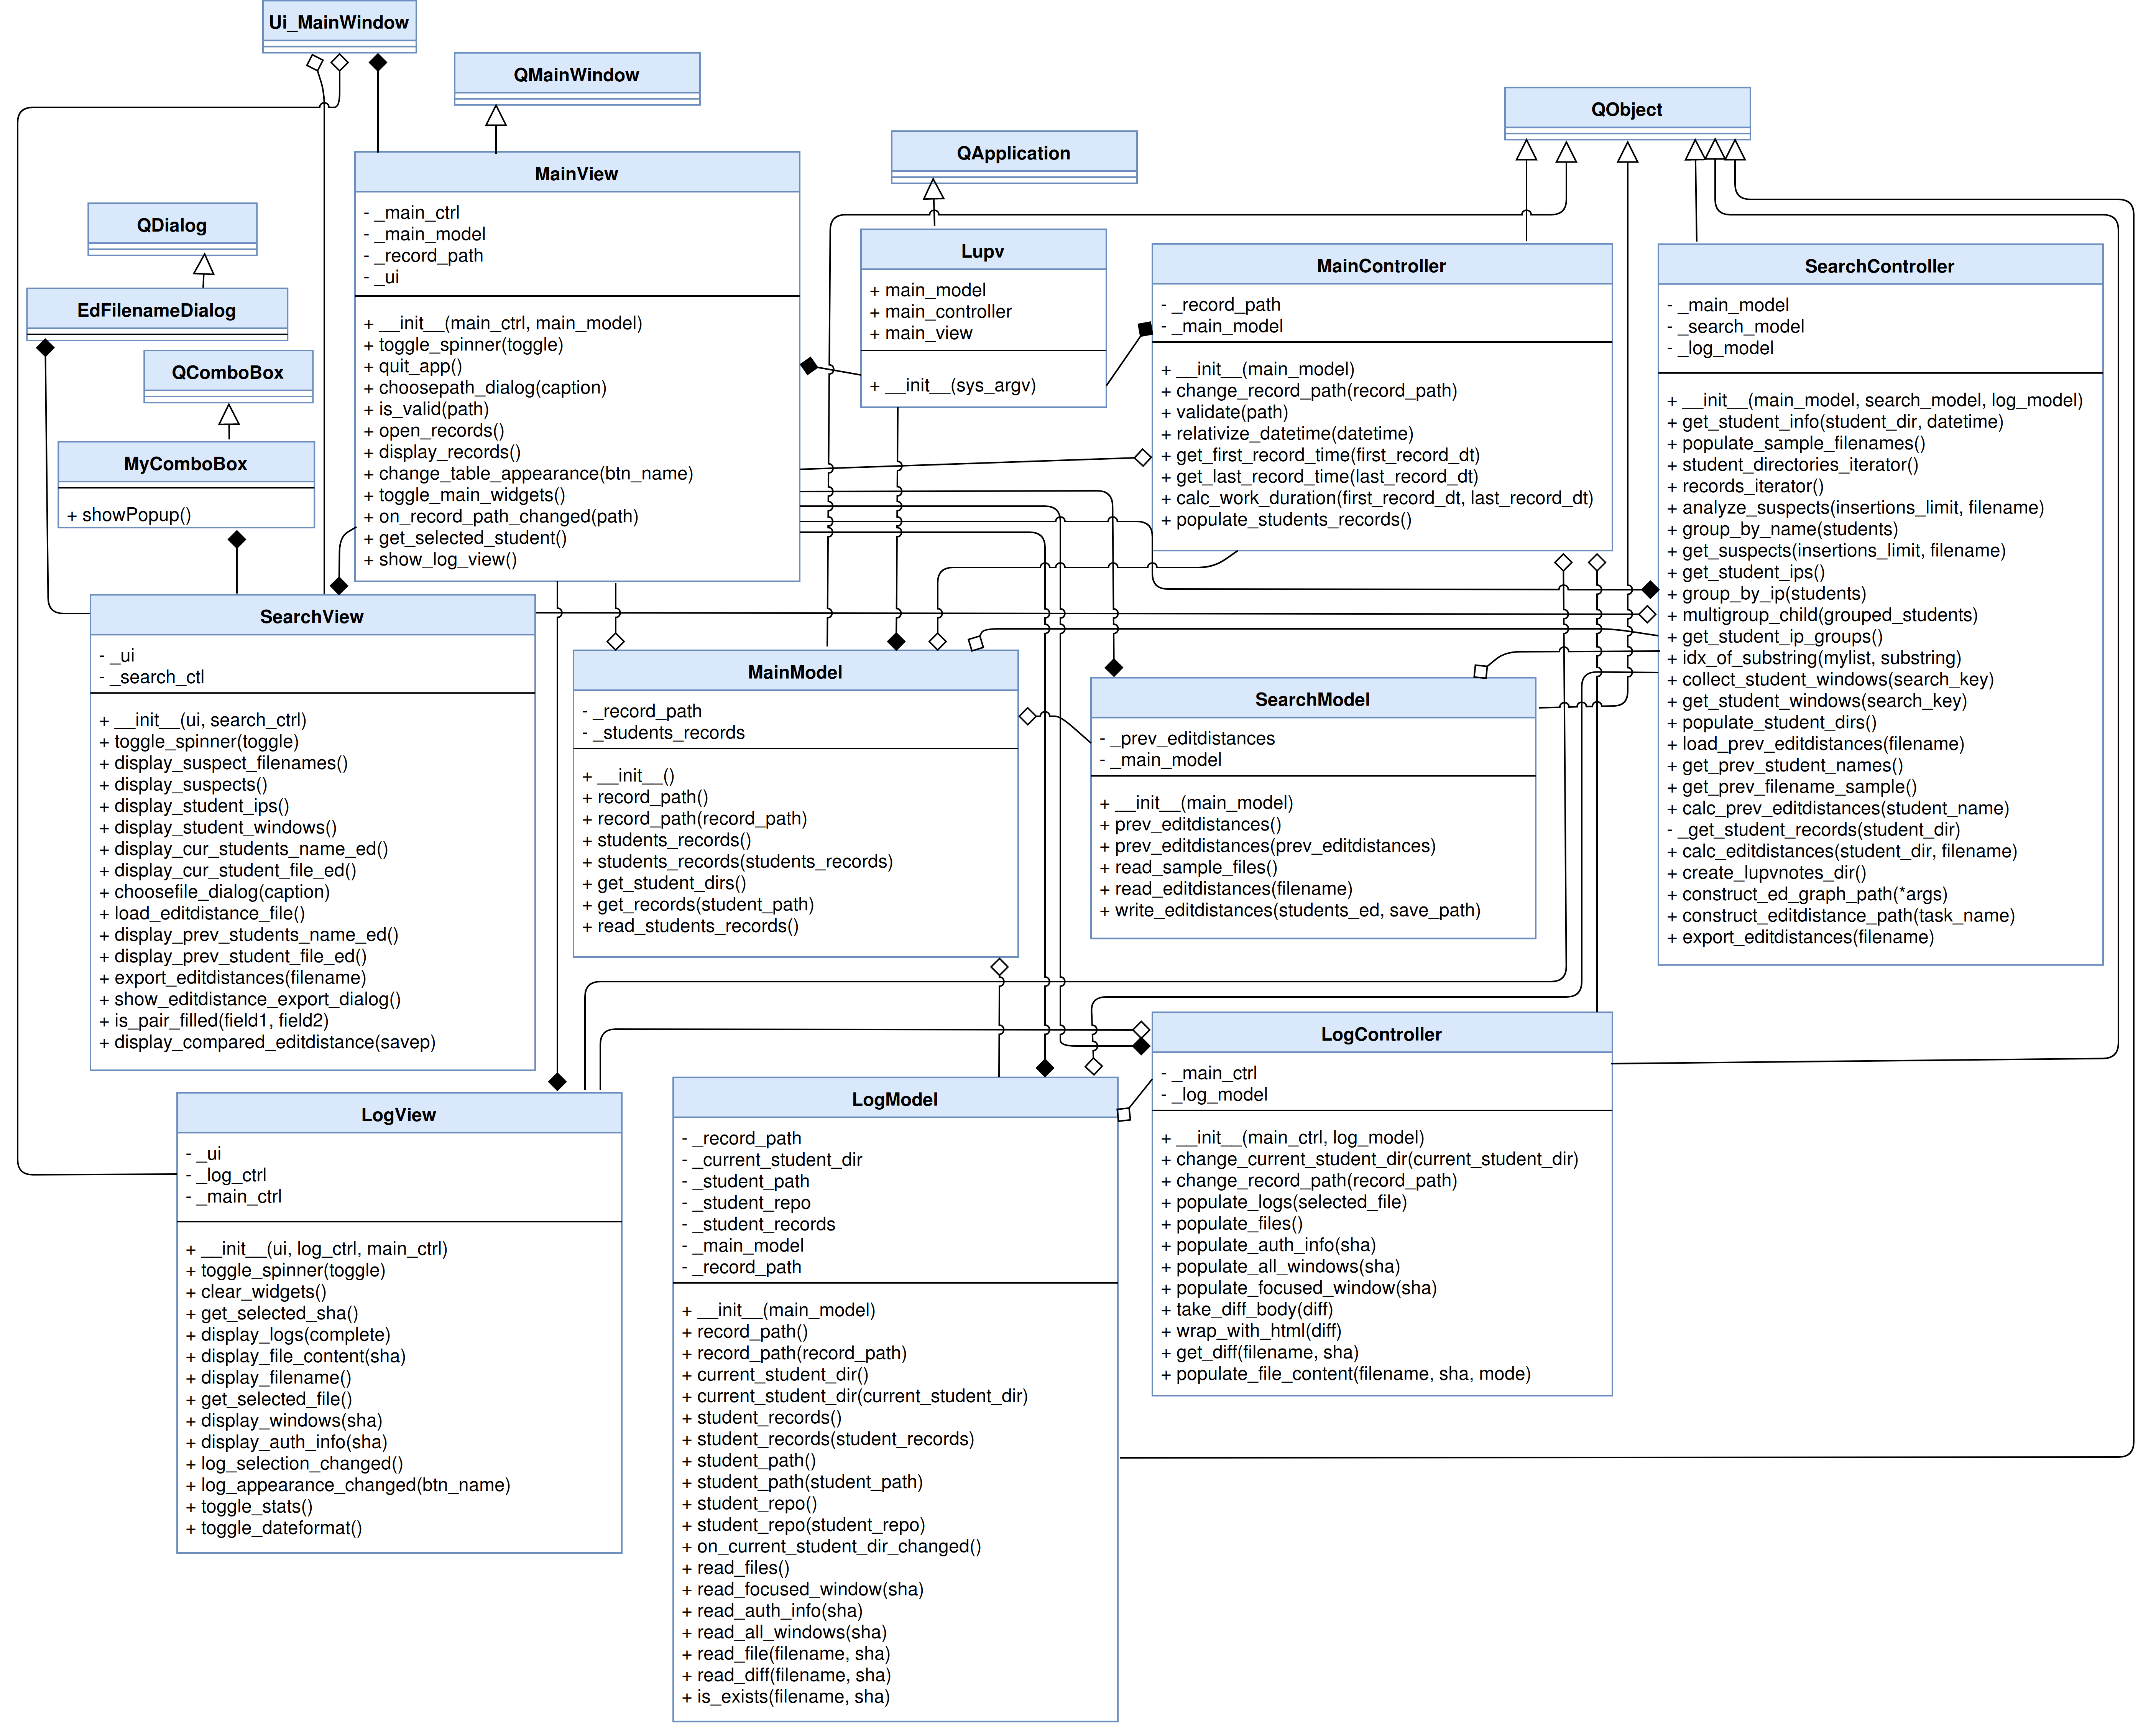
\includegraphics[angle=90,width=1.1\linewidth]{img/use-case/cd/class-lupv-v1_4}
  \caption{Pemodelan \emph{class diagram} \emph{Lup Viewer}}\label{fig:class-lupv}
\end{figure}

\subsection{Perancangan Komponen}

Pada tahapan perancangan komponen, komponen-komponen yang membentuk
sistem akan dirancang menggunakan \emph{pseudocode}. Komponen yang
membentuk sistem dalam sistem berorientasi objek adalah \emph{class}. Maka
tahapan ini akan memaparkan perancangan tiga sampel \emph{class}. Tidak semua
\emph{procedure} atau \emph{function} di dalam suatu \emph{class} akan
dipaparkan, melainkan hanya satu sampel \emph{function} dari tiap-tiap
\emph{class}. Tabel Kode~\ref{pc:get_all_windows} memaparkan \emph{pseudocode} untuk \emph{function}
\emph{get\_all\_windows} dari \emph{class} \emph{Controller} pada sistem \emph{Lup
  Recorder}. Tabel Kode~\ref{pc:populate_logs} memaparkan \emph{pseudocode} untuk
\emph{function} \emph{populate\_logs} dari \emph{class} \emph{LogController} pada
sistem \emph{Lup Viewer} dan, Tabel Kode~\ref{pc:construct-graph-path} memaparkan
\emph{pseudocode} untuk \emph{function} \emph{construct\_ed\_graph\_path}
dari \emph{class} \emph{SearchController} pada sistem \emph{Lup Viewer}.

\subsubsection{Perancangan Komponen \emph{Class} \emph{Controller}}

Pada Tabel Kode~\ref{pc:get_all_windows} dipaparkan \emph{pseudocode}
\emph{get\_all\_windows} pada sistem \emph{Lup
  Recorder}. \emph{Pseudocode} \emph{get\_all\_windows} dirancang
untuk membaca seluruh \emph{window} yang sedang dibuka. Sistem operasi
memiliki banyak atribut selain nama \emph{window}, maka
\emph{get\_all\_windows} hanya mengambil nilai nama \emph{window} dan
mengembalikannya.

\par\null\par
\begin{code}
\begin{ignasicblock}[title=get\_all\_windows,minted language=text]
START
  READ all_windows_dirty
  IF all_windows_dirty is true
    SET all_windows_dirty to split every line
    FOR each window in all_windows_dirty
      GET window_name
      SET all_windows = window_name
    ENDFOR
  ENDIF
  RETURN all_windows
END
\end{ignasicblock}
    \captionof{listing}{\emph{Pseudocode function get\_all\_windows}}\label{pc:get_all_windows}
\end{code}

\subsubsection{Perancangan Komponen \emph{Class} \emph{LogController}}

Pada Tabel Kode~\ref{pc:populate_logs} dipaparkan \emph{pseudocode}
\emph{populate\_log} pada sistem \emph{Lup Viewer}. \emph{Pseudocode}
\emph{populate\_log} dirancang untuk membaca seluruh rekaman
mahasiswa, dari setiap rekaman diambil nilai-nilai yang dibutuhkan
di antaranya adalah waktu rekaman, baris yang ditambah, dan baris yang
dihapus.

\par\null\par
\begin{code}
\begin{ignasicblock}[title=populate\_logs,minted language=text]
START
  CALL log_model RETURNING student_records

  FOR each record in student_records
    CALL main_ctrl with relativize_datetime RETURNING relative_time
    GET time
    GET sha
    SET insetion to 0
    SET deletion to 0
    IF selected_file is true
      IF CALL log_model with is_exist RETURNING true
        GET insertion
        GET deletion
      ENDIF
    ENDIF
  ENDFOR
  SET log to (relative_time, time, sha, insertion, deletion)
  RETURN log
END
\end{ignasicblock}
  \captionof{listing}{\emph{Pseudocode function} \emph{populate\_logs}}\label{pc:populate_logs}
\end{code}

\subsubsection{Perancangan Komponen \emph{Class} \emph{SearchController}}

Pada Tabel Kode~\ref{pc:construct-graph-path} dipaparkan
\emph{pseudocode} \emph{construct\_ed\_graph\_path} pada sistem
\emph{Lup Viewer}. \emph{Pseudocode} \emph{construct\_ed\_graph\_path}
dirancang untuk membangun \emph{path} untuk nama grafik
\emph{edit-distance} yang disimpan. \emph{Path} tersebut mengikuti
jumlah mahasiswa yang ada. Jika terdapat lebih dari satu mahasiswa,
maka diberikan ``\_'' sebagai penghubung nama antar mahasiswa.

\par\null\par
\begin{code}
\begin{ignasicblock}[title=construct\_ed\_graph\_path,minted language=text]
START
  CALL main_model RETURNING record_path

  IF passed argument == 1
    SET graph_fmt to argument + ".png"
  ELSE
    SET graph_fmt to argument + "_" + ".png"
  ENDIF
  SET graph_path record_path + "lupv_notes" + graph_fmt
  RETURN graph_path
END
\end{ignasicblock}
    \captionof{listing}{\emph{Pseudocode function}
    \emph{construct\_ed\_graph\_path}}\label{pc:construct-graph-path}
\end{code}

\subsection{Perancangan Antarmuka}

Perancangan antarmuka merupakan proses merancang antarmuka sistem
dengan menggambar gambaran dasar antarmuka sistem. Rancangan antarmuka dibuat
dengan bantuan kakas bantu \emph{draw.io}. Gambaran rancangan
ini nantinya dijadikan landasan implementasi antarmuka. Terdapat tiga
sampel perancangan antarmuka yang akan dipaparkan, yaitu perancangan
antarmuka tampilan \emph{tray} sistem \emph{Lup Recorder}, perancangan
antarmuka tampilan hasil rekaman sistem \emph{Lup Viewer}, dan
perancangan antarmuka tampilan \emph{edit-distance} tugas sebelumnya.

\subsubsection{Perancangan Antarmuka Tampilan \emph{Tray} Pada Sistem \emph{Lup Recorder}}

Gambar~\ref{fig:ui-lupr-tray} merupakan rancangan antarmuka tampilan
\emph{tray} pada sistem \emph{Lup Recorder}. Antarmuka ini merupakan
rancangan antarmuka utama pada sistem \emph{Lup Recoder} dan digunakan untuk
mengakses seluruh menu utama sistem \emph{Lup Recorder}. Penjelasan
komponen-komponen yang terdapat pada rancangan tersebut terdapat pada
Tabel~\ref{tab:ui-lupr-tray}.

\begin{figure}[H]
  \centering
  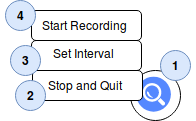
\includegraphics[width=.3\linewidth]{img/ui/ui-lupr-tray}
  \caption{Perancangan antarmuka tampilan \emph{Tray} sistem \emph{Lup
      Recorder}}\label{fig:ui-lupr-tray}
\end{figure}

{\makegapedcells
    \begin{longtable}{|c|L{3.9cm}|L{2cm}|L{6cm}|}
    \caption{Perancangan antarmuka tampilan \emph{Tray} sistem \emph{Lup
        Recorder}}\label{tab:ui-lupr-tray}
    \\\hline
    \thead{No} & \thead{Nama Objek} & \thead{Tipe} & \thead{Keterangan}\\\hline
    %
    1 & \emph{Lup Recorder tray} & Tombol \emph{tray} & Tombol untuk mengakses menu pada sistem \emph{Lup Recorder}. \\\hline
    2 & Tombol ``\emph{Start Recording}'' & Tombol & Tombol memulai merekam tugas. \\\hline
    3 & Tombol ``\emph{Set Interval}'' & Tombol & Tombol mengubah interval rekaman. \\\hline
    4 & Tombol ``Stop and Quit'' & Tombol & Tombol untuk menghentikan perekaman tugas.\\\hline
  \end{longtable}
}

\subsubsection{Perancangan Antarmuka Tampilan Hasil Rekaman Pada Sistem \emph{Lup Viewer}}

Gambar~\ref{fig:ui-lupv-log-view} merupakan rancangan antarmuka
tampilan hasil rekaman pada sistem \emph{Lup Viewer}. Antarmuka ini
merupakan rancangan antarmuka yang digunakan untuk melihat hasil
rekaman. Penjelasan komponen-komponen yang terdapat pada rancangan
tersebut terdapat pada Tabel~\ref{tab:ui-lupv-log-view}.

\begin{figure}[H]
  \centering
  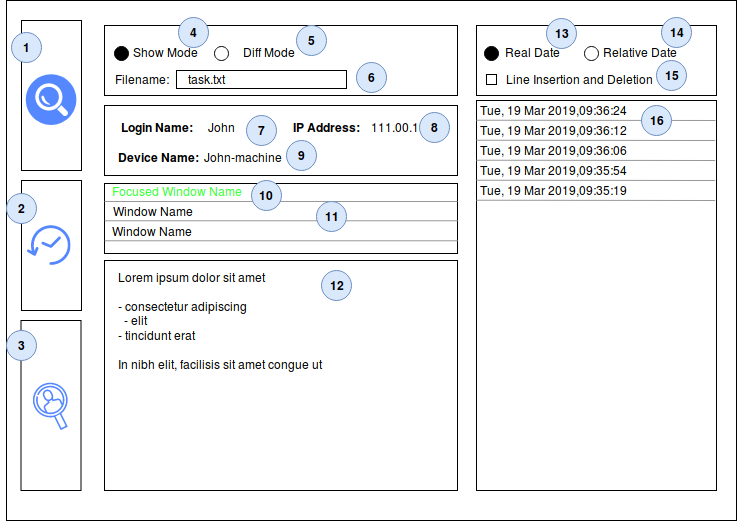
\includegraphics[width=.8\linewidth]{img/ui/ui-lupv-log-view}
  \caption{Perancangan antarmuka tampilan Hasil Rekaman sistem \emph{Lup
      Viewer}}\label{fig:ui-lupv-log-view}
\end{figure}

{\makegapedcells
    \begin{longtable}{|c|L{3.9cm}|L{2cm}|L{6cm}|}
    \caption{Penjelasan antarmuka tampilan Hasil Rekaman sistem \emph{Lup
        Viewer}}\label{tab:ui-lupv-log-view}
    \\\hline
    \thead{No} & \thead{Nama Objek} & \thead{Tipe} & \thead{Keterangan}\\\hline
    %
    1 & Tombol ``\emph{Main View}'' & Tombol & Tombol untuk menuju tampilan utama seluruh daftar rekaman.\\\hline
    2 & Tombol ``\emph{Log View}'' & Tombol & Tombol untuk menuju tampilan hasil rekaman.\\\hline
    3 & Tombol ``\emph{Search View}'' & Tombol & Tombol untuk menuju tampilan analisis hasil rekaman.\\\hline
    4 & Tombol ``\emph{Show Mode}'' & \emph{Radio Button} & \emph{Radio button} untuk mengalihkan mode tampilan rekaman
                                                            berkas ke mode \emph{show}.\\\hline
    5 & Tombol ``\emph{Diff Mode}'' & \emph{Radio Button} & \emph{Radio button} untuk mengalihkan mode tampilan rekaman
                                                            berkas ke mode \emph{diff}.\\\hline
    6 & Tombol ``\emph{Filename}'' & \emph{Combo Box} & \emph{Combo box} untuk memilih nama berkas tugas.\\\hline
    7 & Label ``\emph{Login Name}'' & Label & Label untuk menampilkan nama \emph{login}.\\\hline
    8 & Label ``\emph{Device Name}'' & Label & Label untuk menampilkan nama piranti.\\\hline
    9 & Label ``\emph{IP Address}'' & Label & Label untuk menampilkan alamat \emph{IP}.\\\hline
    10 & Daftar ``\emph{Active Window}'' & \emph{List Widget} & Daftar untuk menampilkan \emph{window}
                                                                yang aktif.\\\hline
    11 & Daftar ``\emph{All Window}'' & \emph{List Widget} & \emph{List widget} untuk menampilkan semua
                                                             \emph{window}.\\\hline
    12 & \emph{Widget} berkas rekaman & \emph{Widget} & \emph{Widget} untuk menampilkan rekaman berkas.\\\hline
    13 & Tombol ``\emph{Real Date}'' & \emph{Radio Button} & \emph{Radio button} untuk mengalihkan mode format waktu
                                                             rekaman ke dalam format waktu \emph{real}.\\\hline
    14 & Tombol ``\emph{Relative Date}'' & \emph{Radio Button} & \emph{Radio button} untuk mengalihkan mode format waktu
                                                                 rekaman ke dalam format waktu relatif.\\\hline
    15 & Tombol ``\emph{Line Insertion and Deletion}'' & \emph{Check Box} & Tombol untuk menampilkan jumlah
                                                                            baris yang ditambah dan dihapus.\\\hline
    16 & Daftar Rekaman & \emph{List Widget} & \emph{List widget} untuk menampilkan daftar rekaman.\\\hline
  \end{longtable}
}

\subsubsection{Perancangan Antarmuka Tampilan \emph{Edit-distance} Tugas Sebelumnya Pada Sistem \emph{Lup Viewer}}

Gambar~\ref{fig:ui-lupv-ed-view} merupakan rancangan antarmuka
tampilan \emph{edit-distance} tugas sebelumnya pada sistem \emph{Lup
  Viewer}. Rancangan antarmuka ini digunakan untuk melihat grafik
\emph{edit-distance} tugas sebelumnya. Penjelasan komponen-komponen
yang terdapat pada rancangan tersebut terdapat pada
Tabel~\ref{tab:ui-lupv-ed-view}.

\begin{figure}[H]
  \centering
  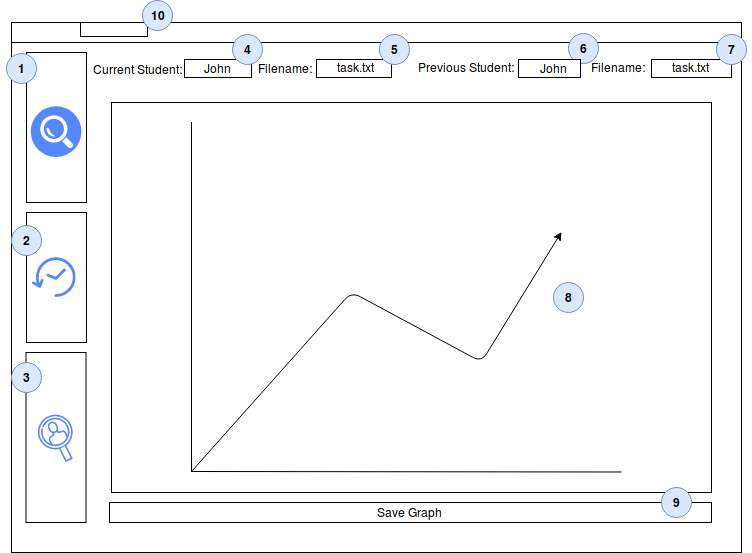
\includegraphics[width=.8\linewidth]{img/ui/ui-lupv-ed-view}
  \caption{Perancangan antarmuka tampilan \emph{Edit-distance} Tugas
    Sebelumnya}\label{fig:ui-lupv-ed-view}
\end{figure}

{\makegapedcells
  \begin{longtable}{|c|L{3.9cm}|L{2cm}|L{6cm}|}
    \caption{Penjelasan antarmuka tampilan \emph{Edit-distance} Tugas
      Sebelumnya}\label{tab:ui-lupv-ed-view}
    \\\hline
    \thead{No} & \thead{Nama Objek} & \thead{Tipe} & \thead{Keterangan}\\\hline
    %
    1 & Tombol ``\emph{Main View}'' & Tombol & Tombol untuk menuju tampilan utama seluruh daftar rekaman.\\\hline
    2 & Tombol ``\emph{Log View}'' & Tombol & Tombol untuk menuju tampilan hasil rekaman.\\\hline
    3 & Tombol ``\emph{Search View}'' & Tombol & Tombol untuk menuju tampilan analisis hasil rekaman.\\\hline
    4 & Tombol ``\emph{Current Student}'' & \emph{Combo Box} & \emph{Combo box} untuk memilih mahasiswa pada tugas saat
                                                               ini.\\\hline
    5 & Tombol ``\emph{Filename}'' & \emph{Combo Box} & \emph{Combo box} untuk memilih berkas tugas saat
                                                               ini.\\\hline
    6 & Tombol ``\emph{Previous Student}'' & \emph{Combo Box} & \emph{Combo box} untuk memilih mahasiswa pada tugas
                                                                sebelumnya.\\\hline
    7 & Tombol ``\emph{Filename}'' & \emph{Combo Box} & \emph{Combo box} untuk memilih mahasiswa pada tugas
                                                        sebelumnya.\\\hline
    8 & \emph{Widget} \emph{Edit-distance} & \emph{Widget} & \emph{Widget} untuk menampilkan grafik
                                                             \emph{edit-distance}.\\\hline
    9 & Tombol ``\emph{Save Graph}'' & Tombol & Tombol untuk menyimpan grafik \emph{edit-distance}.\\\hline
    10 & Tombol ``\emph{Load Edit-distance File}'' & Tombol & Tombol untuk membuka berkas \emph{edit-distance}
                                                              tugas sebelumnya.\\\hline
  \end{longtable}
}


\section{Implementasi Sistem}

Tahapan implementasi sistem merupakan sebuah tahapan yang dilakukan setelah selesainya
proses perancangan sistem. Pada tahapan ini hasil perancangan komponen yang berupa
\emph{pseudocode} diimplementasikan menjadi \emph{working code} menggunakan
bahasa pemrograman \emph{Python} dan bantuan kakas bantu seperti \emph{git}.
Selain itu, Hasil perancangan
antarmuka juga diimplementasikan dengan bantuan \emph{widget toolkit} \emph{Qt}.

\subsection{Spesifikasi Sistem}

Spesifikasi perangkat keras yang digunakan untuk membangun sistem
dipaparkan pada Tabel~\ref{tab:hardware}. Pada Tabel tersebut terdapat
spesifikasi \emph{processor}, \emph{HDD} dan \emph{RAM}. Sementara itu,
spesifikasi perangkat lunak yang digunakan dipaparkan pada
Tabel~\ref{tab:software}, di dalamnya terdapat spesifikasi
sistem operasi, \emph{kernel}, editor dokumentasi, editor pemrograman, dan bahasa
pemrograman.

{\makegapedcells
  \begin{longtable}{|L{4.5cm}|L{6.5cm}|}
   \caption{Spesfikasi perangkat keras} \label{tab:hardware}\\
    \hline
    \thead{Nama Komponen} & \thead{Spesifikasi}\\\hline
    %
    \emph{Processor} & Intel i5-7200U (4) @ 3.1GHz   \\\hline
    \emph{Hard Disk} & 500 GB   \\\hline
    \emph{RAM} & 4 GB    \\\hline
  \end{longtable}
}

{\makegapedcells
  \begin{longtable}{|L{4.5cm}|L{6.5cm}|}
    \caption{Spesfikasi perangkat lunak} \label{tab:software}\\
    \hline
    \thead{Nama Komponen} & \thead{Spesifikasi}\\\hline
    %
    Sistem Operasi & Debian GNU/Linux 9.6 (stretch) x86\_64 \\\hline
    \emph{Kernel} & Kernel: 4.9.0-6-amd64    \\\hline
    Editor Dokumentasi & GNU Emacs 26.1  \\\hline
    Editor Pemrograman & GNU Emacs 26.1  \\\hline
    Bahasa Pemrograman & Python 3.6.4    \\\hline
  \end{longtable}
}

\subsection{Implementasi Kode Program}

Pada tahapan implementasi kode program. Hasil rancangan komponen
sistem pada tahapan perancangan komponen sistem diimplementasikan
menjadi \emph{working code} dengan bahasa pemrograman \emph{Python}.
Subbab 5.2.2.1 hingga 5.2.2.3 memaparkan
implementasi dari tiga sampel \emph{class} pada tahapan perancangan
komponen sebelumnya, yaitu \emph{class} \emph{Controller} pada sistem
\emph{Lup Recorder}, \emph{class} \emph{LogController} pada sistem
\emph{Lup Viewer}, dan \emph{class} \emph{SearchController} pada
sistem \emph{Lup Viewer}.

\subsubsection{Implementasi Kode Program \emph{Class} \emph{Controller} Pada Sistem \emph{Lup Recorder}}

Pada Tabel Kode~\ref{code:get_all_windows} dipaparkan \emph{source
  code} \emph{get\_all\_windows}. \emph{Source code}
\emph{get\_all\_windows} mengimplementasikan hasil rancangan
\emph{pseudocode} pada tahapan sebelumnya. \emph{Source code}
\emph{get\_all\_windows} mengambil seluruh informasi \emph{window}
yang kemudian melakukan filter dan hanya mengembalikan nama
\emph{window} saja.

\par\null\par
\begin{code}
\begin{ignasicblock}[title=get\_all\_windows,minted language=Python]
def get_all_windows(self):
  all_windows = ""
  all_windows_proc = Popen(["wmctrl", "-l"], stdout=PIPE)
  all_windows_dirty, err = all_windows_proc.communicate()
  if all_windows_dirty:
    all_windows_dirty = all_windows_dirty.splitlines()
    for line in all_windows_dirty:
      windows_name = line.split(None, 3)[-1].decode()
      all_windows += "{}\n".format(windows_name)
  return all_windows
\end{ignasicblock}
    \captionof{listing}{Source code \emph{function get\_all\_windows}}\label{code:get_all_windows}
\end{code}

\subsubsection{Implementasi Kode Program \emph{Class} \emph{LogController} Pada Sistem
  \emph{Lup Viewer}}

Pada Tabel Kode~\ref{code:populate_logs} dipaparkan \emph{source code}
\emph{populate\_log}. \emph{Source code} \emph{populate\_log}
mengimplementasikan hasil rancangan \emph{pseudocode} pada tahapan
sebelumnya. \emph{Source code} \emph{populate\_log} membaca seluruh
rekaman mahasiswa, dari setiap rekaman diambil nilai-nilai yang
dibutuhkan di antaranya adalah waktu rekaman, baris yang ditambah, dan
baris yang dihapus.

\par\null\par
\begin{code}
\begin{ignasicblock}[title=populate\_logs,minted language=Python]
def populate_logs(self, selected_file=None):
  student_records = self._log_model.student_records

  for record in student_records:
    relative_time = self._main_ctrl.relativize_datetime(
      record.committed_datetime
    )
    time_format = "{:%a, %d %b %Y, %H:%M:%S}"
    time = time_format.format(record.committed_datetime)
    sha = record.hexsha
    insertions = 0
    deletions = 0

    if selected_file:
      if self._log_model.is_exists(selected_file, sha):
        insertions = record.stats.files[selected_file]["insertions"]
        deletions = record.stats.files[selected_file]["deletions"]

    log = dict(
      relative_time=relative_time,
      time=time,
      sha=sha,
      insertions=insertions,
      deletions=deletions,
    )
    yield log
\end{ignasicblock}
    \captionof{listing}{Source code \emph{function populate\_logs}}\label{code:populate_logs}
\end{code}

\subsubsection{Implementasi Kode Program \emph{Class} \emph{SearchController} Pada Sistem
  \emph{Lup Viewer}}

Pada Tabel Kode~\ref{code:populate_logs} dipaparkan \emph{source code}
\emph{construct\_ed\_graph\_path}. \emph{Source code}
\emph{construct\_ed\_graph\_path} mengimplementasikan hasil rancangan
\emph{pseudocode} pada tahapan sebelumnya. \emph{Source code}
\emph{construct\_ed\_graph\_path} membangun \emph{path} untuk nama
grafik \emph{edit-distance} yang disimpan. \emph{Path} tersebut
mengikuti jumlah mahasiswa yang ada. Jika terdapat lebih dari satu
mahasiswa, maka diberikan ``\_'' sebagai penghubung nama antar
mahasiswa.

\par\null\par
\begin{code}
\begin{ignasicblock}[title=construct\_ed\_graph\_path,minted language=Python]
def construct_ed_graph_path(self, *args):
  record_path = self._main_model.record_path

  if len(args) == 1:
    graph_fmt = "{}.png".format(args[0])
  else:
    names = "_".join(args)
    graph_fmt = "{}.png".format(names)

  graph_path = join(record_path, "lupv-notes", graph_fmt)
  return graph_path
\end{ignasicblock}
  \captionof{listing}{\emph{Source code} \emph{function construct\_ed\_graph\_path}}\label{code:load_data}
\end{code}

\subsection{Implementasi Antarmuka}

Pada Tahapan ini, hasil rancangan antarmuka pada tahapan sebelumnya
diimplementasikan menggunakan \emph{widget toolkit} \emph{Qt}.
Tiga sampel implementasi antarmuka yang dipaparkan adalah antarmuka tampilan
\emph{tray} pada sistem \emph{Lup Recorder} pada
Gambar~\ref{fig:ss-lupr-tray}, antarmuka tampilan hasil rekaman pada
sistem \emph{Lup Viewer} pada Gambar~\ref{fig:ss-lupv-log-view}, dan
antarmuka tampilan \emph{edit-distance} tugas sebelumnya pada sistem
\emph{Lup Viewer} pada Gambar~\ref{fig:ss-lupv-ed-view}.

\subsubsection{Implementasi Antarmuka Tampilan \emph{Tray} Pada Sistem \emph{Lup Recorder}}

Gambar~\ref{fig:ss-lupr-tray} merupakan implementasi antarmuka
tampilan \emph{tray} pada sistem \emph{Lup Recorder}. Implementasi ini
dibangun berlandaskan tahapan perancangan antarmuka
sebelumnya. Antarmuka ini merupakan rancangan antarmuka utama pada
sistem \emph{Lup Recoder} dan digunakan untuk mengakses seluruh menu
utama sistem \emph{Lup Recorder}.

\begin{figure}[H]
  \centering
  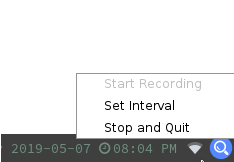
\includegraphics[width=.5\linewidth]{img/ui/ss-lupr-tray}
  \caption{Implementasi antarmuka tampilan \emph{Tray} pada sistem
    \emph{Lup Recorder}}\label{fig:ss-lupr-tray}
\end{figure}

\subsubsection{Implementasi Antarmuka Tampilan Hasil Rekaman Pada Sistem \emph{Lup Viewer}}

Gambar~\ref{fig:ss-lupv-log-view} merupakan implementasi antarmuka
tampilan hasil rekaman pada sistem \emph{Lup Viewer}. Implementasi ini
dibangun berlandaskan tahapan perancangan antarmuka
sebelumnya. Antarmuka ini merupakan rancangan antarmuka yang digunakan
untuk melihat hasil rekaman.

\begin{figure}[tph]
  \centering
  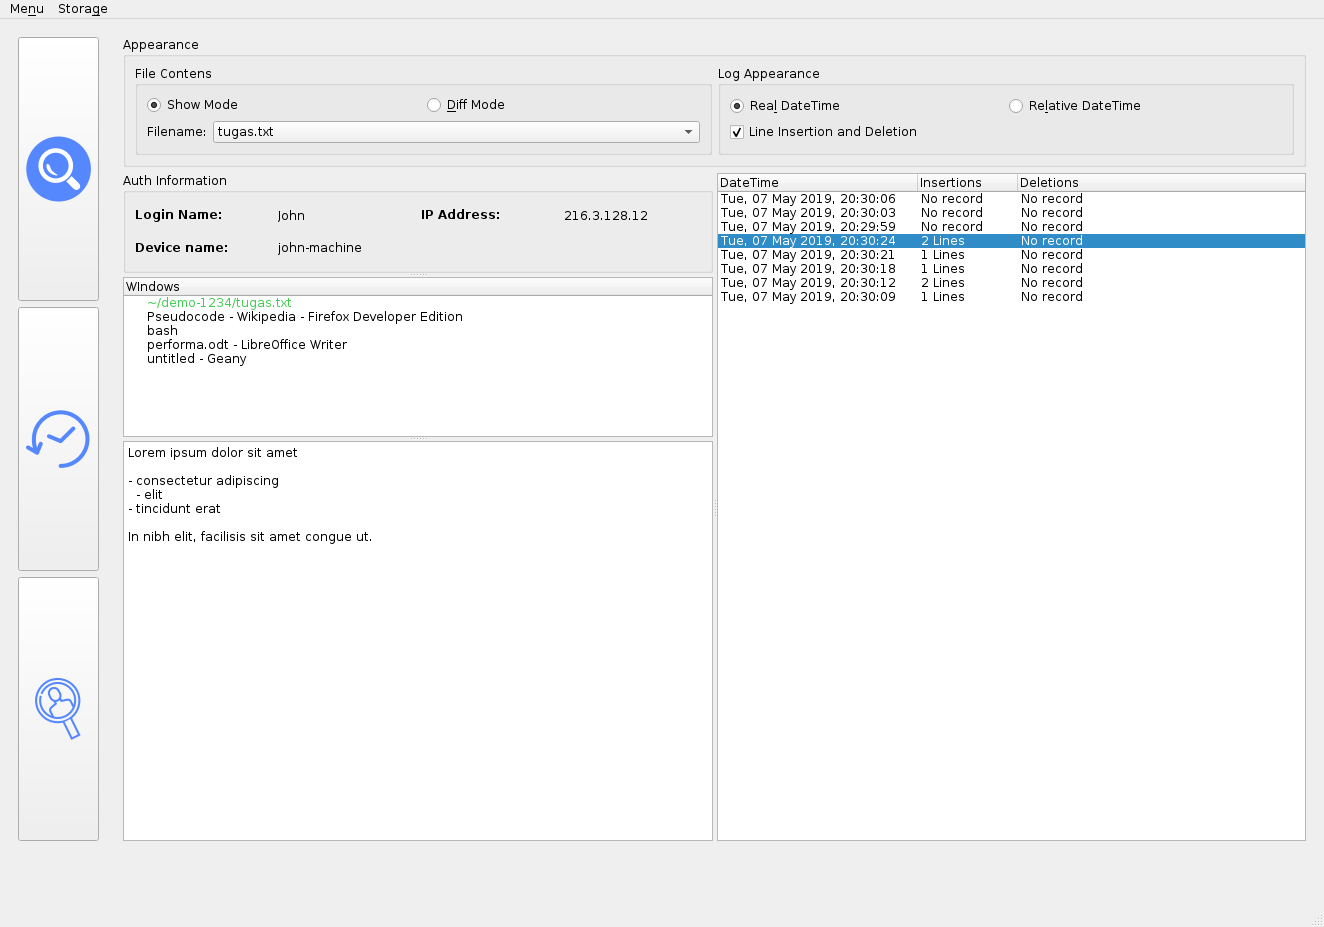
\includegraphics[width=.9\linewidth]{img/ui/ss-lupv-log-view}
  \caption{Implementasi antarmuka tampilan Hasil Rekaman pada sistem \emph{Lup
      Viewer}}\label{fig:ss-lupv-log-view}
\end{figure}

\subsubsection{Perancangan Antarmuka Tampilan \emph{Edit-distance} Tugas Sebelumnya Pada Sistem \emph{Lup Viewer}}

Gambar~\ref{fig:ss-lupv-ed-view} merupakan implementasi antarmuka
tampilan \emph{edit-distance} tugas sebelumnya pada sistem \emph{Lup
  Viewer}. Implementasi ini dibangun berlandaskan tahapan perancangan
antarmuka sebelumnya. Antarmuka ini digunakan untuk melihat grafik
\emph{edit-distance} tugas sebelumnya.

\begin{figure}[tph]
  \centering
  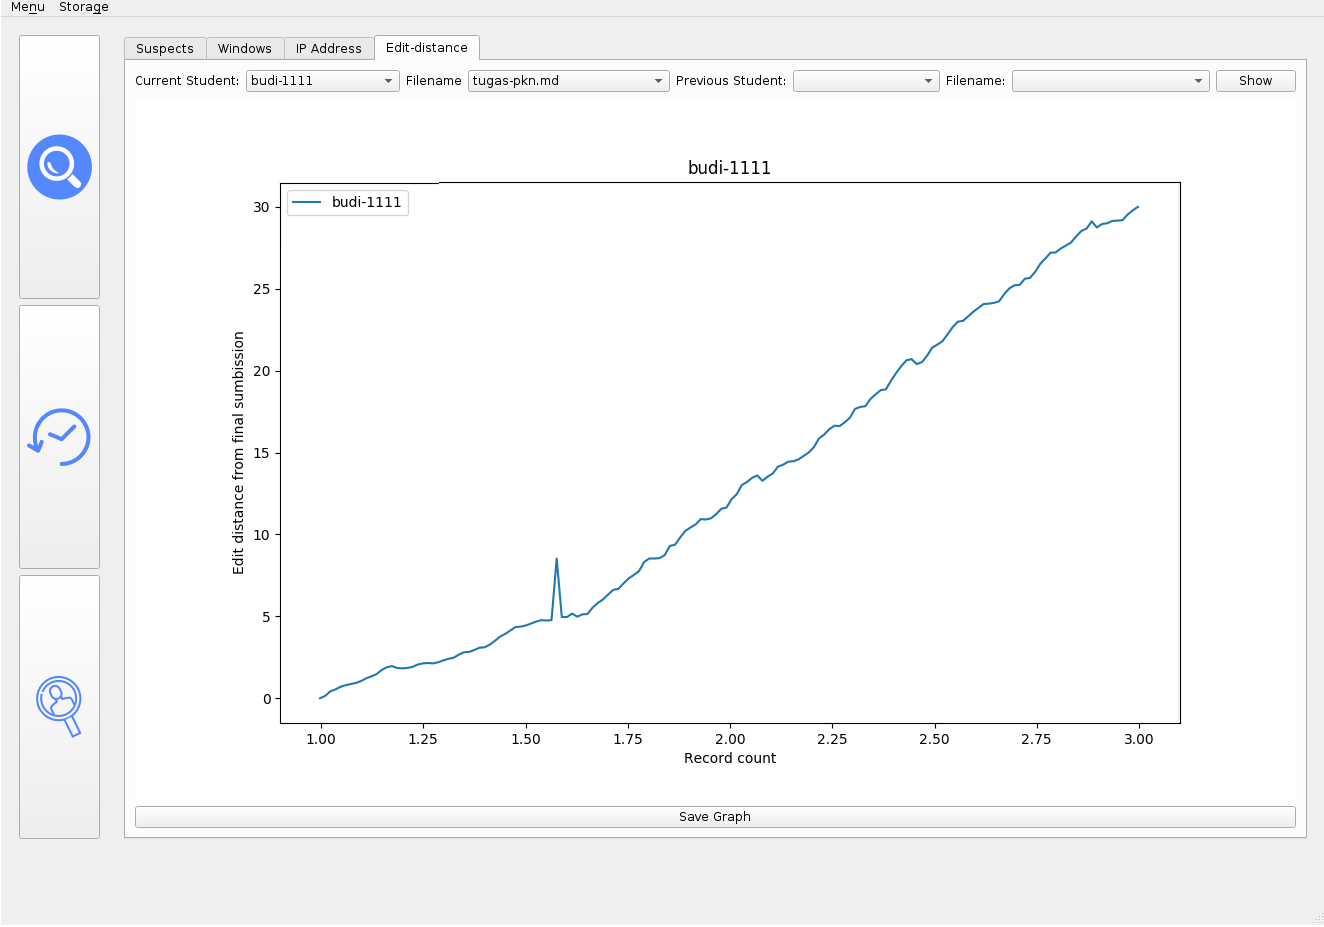
\includegraphics[width=.9\linewidth]{img/ui/ss-lupv-ed-view}
  \caption{Perancangan antarmuka tampilan \emph{Edit-distance} Tugas Sebelumnya
    pada sistem \emph{Lup Viewer}}\label{fig:ss-lupv-ed-view}
\end{figure}


%%% Local Variables:
%%% coding: utf-8
%%% mode: latex
%%% TeX-engine: xetex
%%% TeX-master: "skripsi"
%%% ispell-local-dictionary: "id"
%%% End:

%%%%%%%%%%%%%%%%%%%%%%%%%%%%%%%%%%%%%%%%%%%%%%%%%%%%%%%%%%%%%%%%%%%%%%%

% BAB 6
%%%%%%%%%%%%%%%%%%%%%%%%%%%%%%%%%%%%%%%%%%%%%%%%%%%%%%%%%%%%%%%%%%%%%%%

\mychapter{6}{BAB 6 PENGUJIAN}

\section{Pengujian Unit}

Pengujian unit dilakukan untuk memastikan hasil implementasi kode program telah
sesuai dengan hasil perancangan komponen. Komponen terkecil dari sebuah sistem
berorientasi objek adalah \emph{class} dengan \emph{testable unit} terkecilnya
adalah \emph{function} atau \emph{method}
\parencite{pressman2010software}. Pengujian unit pada \emph{class model} dan
\emph{class controller} dilakukan hingga mencapai 100\% \emph{code
  coverage}. \emph{Class} \emph{view} hanya memanggil fungsi-fungsi
yang terdapat pada \emph{class} \emph{controller} dan \emph{class model} sehingga pada
penelitian ini pengujian unit pada \emph{class} \emph{view} hanya diuji hingga
\emph{code coverage} mencapai 70\%. Metode pengujian yang digunakan adalah
\emph{white-box testing}, dan teknik pengujian yang digunakan adalah
\emph{basis path testing}. \emph{Driver} digunakan sebagai
\emph{``main program''} untuk memanggil \emph{function} yang diuji.
\emph{Stub} atau \emph{fake} digunakan agar pengujian unit benar-benar
terisolasi, bukan sebagai \emph{``stand-alone program''}.
Terdapat tiga sampel pengujian unit yang akan di paparkan pada tahapan
ini. Gambar~\ref{fig:unit-test-coverage} memperlihatkan hasil pengujian unit pada \emph{class controller}
dan \emph{class model} yang mencapai 100\% \emph{code coverage}.

\begin{figure}[tph]
  \centering
  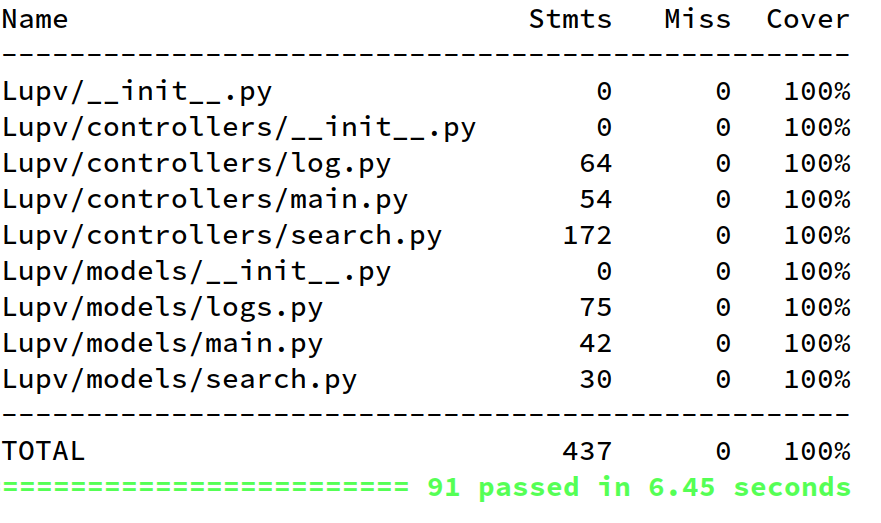
\includegraphics[width=.6\linewidth]{img/unit-test-coverage-cropped}
  \caption{Pengujian unit mencapai 100\% \emph{code coverage}}
  \label{fig:unit-test-coverage}
\end{figure}

\subsection{Pengujian Unit \emph{Class} \emph{Controller} \emph{Function} \emph{get\_all\_windows}}

Pengujian \emph{unit} dilakukan pada \emph{function}
\emph{get\_all\_windows} secara terisolasi. Maka unit lain
yang dipanggil di dalamnya akan digantikan dengan \emph{stub}.
Tabel Kode~\ref{pct:get_all_windows} dan Gambar~\ref{fg:get_all_windows}
menjelaskan \emph{basis path} dari \emph{pseudocode}
\emph{function} \emph{get\_all\_windows}. Bagian berikutnya menjelaskan
perhitungan \emph{cyclomatic complexity}, dan \emph{independent path}.
Tabel~\ref{jalur:get_all_windows} menjelaskan hasil uji dan kasus uji
dari \emph{function} \emph{get\_all\_windows}.

\par\null\par
\begin{code}
\begin{ignasicblock}[title=get\_all\_windows,minted language=text,
underlay={
  \drawline{8cm}{11.5cm}{2.5}{1}
  \drawline{8cm}{12.5cm}{3.5}{2}
  \drawline{12cm}{11.5cm}{5}{3}
  \drawline{10cm}{12.5cm}{6}{4}
  \drawbrace{12cm}{6.5}{8.5}{5}
  \drawline{8cm}{11.5cm}{10}{6}
  \drawline{8cm}{12.5cm}{11}{7}
  \drawline{8cm}{11.5cm}{12.5}{8}
 }]

START
  READ all_windows_dirty
  IF all_windows_dirty is true
    SET all_windows_dirty to split every line
    FOR each window in all_windows_dirty
      GET window_name
      SET all_windows = window_name
    ENDFOR
  ENDIF
  RETURN all_windows
END
\end{ignasicblock}
  \captionof{listing}{\emph{Pseudocode function}
    \emph{get\_all\_windows}}\label{pct:get_all_windows}
\end{code}

\begin{figure}[H]
  \centering
  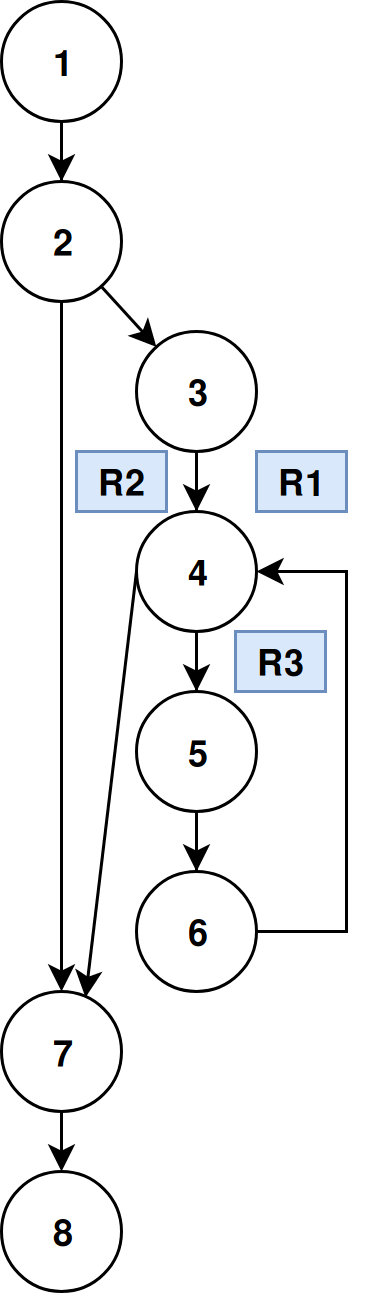
\includegraphics[width=.19\linewidth]{img/test-case/fg-get_all_windows-v2}
  \caption{\emph{Flow graph} dari \emph{pseudocode}
    \emph{get\_all\_windows}}\label{fg:get_all_windows}
\end{figure}

\noindent
\emph{Cyclomatic Complexity}

\begin{itemize}
\item V(G) = 3 \emph{regions}
\item V(G) = 9 \emph{edge} – 8 \emph{node} + 2 = 3
\item V(G) = 2 \emph{predicate node} + 1 = 3
\end{itemize}
\newpage % manual-adj
\noindent
\emph{Independent Path}

\begin{itemize}
\item Jalur 1 : 1 - 2 - 7 - 8
\item Jalur 2 : 1 - 2 - \textbf{3 - 4} - 7 - 8
\item Jalur 2 : 1 - 2 - 3 - 4 - \textbf{5 - 6} - 4 - 7 - 8
\end{itemize}

\begin{longtable}{|P{.06\textwidth}|P{.30\textwidth}|P{.30\textwidth}|P{.10\textwidth}|P{.08\textwidth}|}
  \caption{Kasus uji dan hasil uji \emph{function get\_all\_windows}}\label{jalur:get_all_windows}\\\hline
  \textbf{Jalur} & \textbf{Prosedur Uji} & \textbf{\emph{Expected Result}} & \textbf{\emph{Result}} & \textbf{Status} \\\hline
  %
  1 & 1) \emph{Set variable window\_title} dengan nilai ``None''.\par\null\par
      2) \emph{Class Driver TestController} memanggil \emph{function get\_all\_windows}
                                         & \emph{Return value} \emph{function get\_all\_windows} bernilai
                                           ``\texttt{""}''. & \emph{As expected} & Valid \\\hline
                                           %
  2 & 1) \emph{Set variable window\_title} dengan nilai ``\texttt{""}''.\par\null\par
      2) \emph{Class Driver TestController} memanggil \emph{function get\_all\_windows}.
                                         & \emph{Return value} \emph{function get\_all\_windows} bernilai
                                           ``\texttt{""}''. & \emph{As expected} & Valid \\\hline
                                           %
  3 & 1) \emph{Set variable window\_title} dengan nilai ``b\texttt{"}0x006000ab  0 machine-name
      foo\_window\_title \texttt{"}''.\par\null\par
      2) \emph{Class Driver TestController} memanggil \emph{function get\_all\_windows}.
                                         & \emph{Return value} \emph{function get\_all\_windows} bernilai
                                           ``foo\_window\_title'' & \emph{As expected} & Valid \\\hline
                                           %
  %
\end{longtable}

Pengujian unit yang dilakukan pada \emph{function} \emph{get\_all\_windows}
menghasilkan perhitungan \emph{cyclomatic complexity} dengan nilai 3 sehingga
memiliki 3 \emph{independent path} yang harus diuji. Hasil pengujian 3
\emph{path} yang dipaparkan pada Tabel~\ref{jalur:get_all_windows} bernilai valid.

\subsection{Pengujian Unit \emph{Class} \emph{LogController}
  \emph{Function} \emph{populate\_logs}}

Pengujian \emph{unit} dilakukan pada \emph{function}
\emph{populate\_logs} secara terisolasi. Maka \emph{function
  student\_record}, \emph{function is\_exist} pada unit \emph{LogModel},
dan \emph{function relativize\_datetime} pada unit
\emph{MainController} yang dipanggil di dalamnya akan digantikan
dengan \emph{stub}. Tabel Kode~\ref{pct:populate_logs} dan
Gambar~\ref{fg:populate_logs} menjelaskan \emph{basis path} dari
\emph{pseudocode} \emph{function} \emph{populate\_logs}. Bagian
berikutnya menjelaskan perhitungan \emph{cyclomatic complexity} dan
\emph{independent path}. Tabel~\ref{jalur:populate_logs} menjelaskan
hasil uji dan kasus uji dari \emph{function} \emph{populate\_logs}.

\par\null\par
\begin{code}
\begin{ignasicblock}[title=populate\_logs,minted language=text,
underlay={
  \drawline{10cm}{12cm}{2.5}{1}
  \drawline{9cm}{12.5cm}{5}{2}
  \drawbrace{12cm}{5.5}{12.5}{3}
  \drawline{10cm}{12.5cm}{13.5}{4}
  \drawline{10.5cm}{12cm}{16}{5}
  \drawbrace{12cm}{16.5}{18.7}{6}
  \drawline{6.5cm}{12.8cm}{19.6}{7}
  \drawline{6.5cm}{12cm}{21}{8}
  \drawline{6.5cm}{12.8cm}{22}{9}
  \drawbrace{12cm}{23}{26}{10}
 }]

START
  CALL log_model RETURNING student_records

  FOR each record in student_records
    CALL main_ctrl with relativize_datetime \
                         RETURNING relative_time
    GET time
    GET sha
    SET insetion to 0
    SET deletion to 0
    IF selected_file is true
      IF CALL log_model with is_exist \
                             RETURNING true
        GET insertion
        GET deletion
      ENDIF
    ENDIF
  ENDFOR
  SET log to (relative_time, time, sha,
                   insertion, deletion)
  RETURN log
END
\end{ignasicblock}
  \captionof{listing}{\emph{Pseudocode function}
    \emph{populate\_logs}}\label{pct:populate_logs}
\end{code}

\begin{figure}[H]
  \centering
  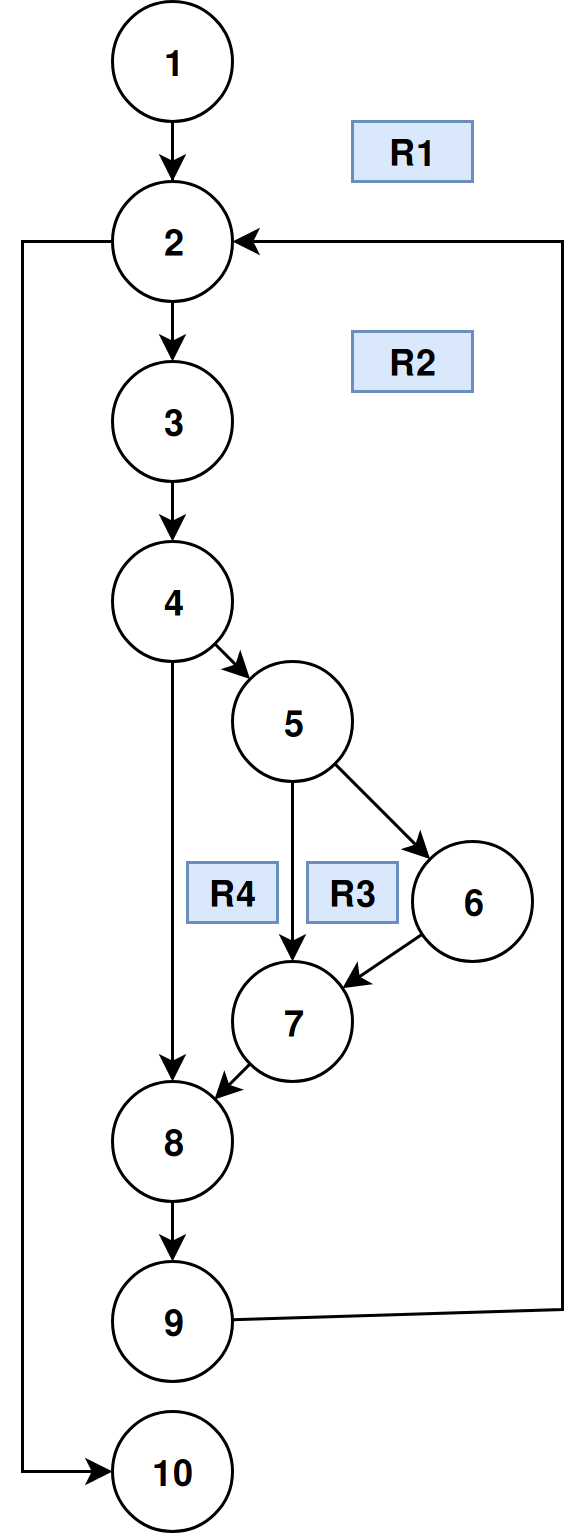
\includegraphics[width=.3\linewidth]{img/test-case/populate-logs}
  \caption{\emph{Flow graph} dari \emph{pseudocode}
    \emph{pupoulate\_logs}}\label{fg:populate_logs}
\end{figure}

\noindent
\emph{Cyclomatic Complexity}

\begin{itemize}
\item V(G) = 4 \emph{regions}
\item V(G) = 12 \emph{edge} – 10 \emph{node} + 2 = 4
\item V(G) = 3 \emph{predicate node} + 1 = 4
\end{itemize}

\noindent
\emph{Independent Path}

\begin{itemize}
\item Jalur 1: 1 - 2 - 10
\item Jalur 2: 1 - 2 - \textbf{3 - 4 - 8 - 9} - 2 - 10
\item Jalur 3: 1 - 2 - 3 - 4 - \textbf{5 - 7} - 8 - 9 - 2 - 10
\item Jalur 4: 1 - 2 - 3 - 4 - 5 - \textbf{6} - 7 - 8 - 9 - 2 - 10
\end{itemize}
\newpage % manual-adj
\begin{longtable}{|P{.06\textwidth}|P{.30\textwidth}|P{.30\textwidth}|P{.10\textwidth}|P{.08\textwidth}|}
  \caption{Kasus uji dan hasil uji \emph{function populate\_logs}} \label{jalur:populate_logs}\\
  \hline
  \textbf{Jalur} & \textbf{Prosedur Uji} & \textbf{\emph{Expected Result}} & \textbf{\emph{Result}} & \textbf{Status} \\\hline
  %
  1 & 1) \emph{Set variable student\_records} dengan nilai ``[]''.\par\null\par
      2) \emph{Class Driver TestLogController} memanggil \emph{function populate\_logs}.
                                         & \emph{Return value} \emph{function populate\_logs} bernilai
                                           ``[]''. & \emph{As expected} & Valid \\\hline
                                           %
  2 & \emph{Class Driver TestLogController} memanggil \emph{function populate\_logs} tanpa \emph{argument}.
                                         & \emph{Return value} \emph{function populate\_logs} bernilai data
                                           rekaman tanpa nilai baris yang ditambah dan dihapus.
                                                                           & \emph{As expected} & Valid \\\hline
                                           %
  3 & \emph{Class Driver TestLogController} memanggil \emph{function populate\_logs} dengan \emph{argument}
      ``selected\_file=\texttt{"}tugas-none.txt\texttt{"}''. & \emph{Return value} \emph{function populate\_logs} bernilai data
                                                               rekaman tanpa nilai baris yang ditambah dan dihapus.
                                                                           & \emph{As expected} & Valid \\\hline
  %
  4 & \emph{Class Driver TestLogController} memanggil \emph{function populate\_logs} dengan \emph{argument}
      ``selected\_file=\texttt{"}tugas-tif.txt\texttt{"}''. & \emph{Return value} \emph{function populate\_logs} bernilai data
                                                               rekaman dengan nilai baris yang ditambah dan dihapus.
                                                                           & \emph{As expected} & Valid \\\hline
  %
\end{longtable}

Pengujian unit yang dilakukan pada \emph{function populate\_logs}
menghasilkan perhitungan \emph{cyclomatic complexity} dengan nilai 4 sehingga
memiliki 4 \emph{independent path} yang harus diuji. Hasil pengujian 4
\emph{path} yang dipaparkan pada Tabel~\ref{jalur:populate_logs} bernilai valid.

\subsection{Pengujian Unit \emph{Class} \emph{SearchController} \emph{Function} \newline
  \emph{construct\_ed\_graph\_path}}

Pengujian \emph{unit} dilakukan pada \emph{function}
\emph{construct\_ed\_graph\_path} secara terisolasi. Maka unit
\emph{main\_model} yang dipanggil di dalamnya akan digantikan
dengan \emph{stub}. Tabel Kode~\ref{pct:construct_ed_graph_path} dan
Gambar~\ref{fg:construct_ed_graph_path} menjelaskan \emph{basis path}
dari \emph{pseudocode} \emph{function} \emph{construct\_ed\_graph\_path}. Bagian
berikutnya menjelaskan perhitungan \emph{cyclomatic complexity},
dan \emph{independent path}.  Tabel~\ref{jalur:construct_ed_graph_path} menjelaskan
hasil uji dan kasus uji dari \emph{function} \emph{construct\_ed\_graph\_path}.

\par\null\par
\begin{code}
\begin{ignasicblock}[title=construct\_ed\_graph\_path,minted language=text,
underlay={
  \drawline{10cm}{11.5cm}{2.3}{1}
  \drawline{10cm}{12.5cm}{4.5}{2}
  \drawline{10cm}{11.5cm}{6}{3}
  \drawline{11cm}{12.5cm}{8.5}{4}
  \drawline{7cm}{11.5cm}{9.8}{5}
  \drawbrace{11.5cm}{10.5}{13.5}{6}
 }]

START
  CALL main_model RETURNING record_path

  IF passed argument == 1
    SET graph_fmt to argument + ".png"
  ELSE
    SET graph_fmt to argument + "_" + ".png"
  ENDIF
  SET graph_path record_path + "lupv_notes" \
                                  + graph_fmt
  Return graph_path
END
\end{ignasicblock}
  \captionof{listing}{\emph{Pseudocode function}
    \emph{construct\_ed\_graph\_path}}\label{pct:construct_ed_graph_path}
\end{code}

\begin{figure}[H]
  \centering
  \includegraphics[width=.23\linewidth]{img/test-case/construct_ed_graph_path}
  \caption{\emph{Flow graph} dari \emph{pseudocode}
    \emph{construct\_ed\_graph\_path}}\label{fg:construct_ed_graph_path}
\end{figure}
\newpage % manual-adj
\noindent
\emph{Cyclomatic Complexity}

\begin{itemize}
\item V(G) = 2 \emph{regions}
\item V(G) = 6 \emph{edge} – 6 \emph{node} + 2 = 2
\item V(G) = 1 \emph{predicate node} + 1 = 2
\end{itemize}

\noindent
\emph{Independent Path}

\begin{itemize}
\item Jalur 1: 1 - 2 - 3 - 5 - 6
\item Jalur 2: 1 - 2 - \textbf{4} - 5 - 6
\end{itemize}

\begin{longtable}{|P{.06\textwidth}|P{.30\textwidth}|P{.30\textwidth}|P{.10\textwidth}|P{.08\textwidth}|}
  \caption{Kasus uji dan hasil uji \emph{function construct\_ed\_graph\_path}} \label{jalur:construct_ed_graph_path}\\
  \hline
  \textbf{Jalur} & \textbf{Prosedur Uji} & \textbf{\emph{Expected Result}} & \textbf{\emph{Result}} & \textbf{Status} \\\hline
  %
  1 & \emph{Class Driver TestSearchController} memanggil \emph{function construct\_ed\_graph\_path} dengan
      \emph{argument} ``ani-1111''. & \emph{Return value} \emph{function construct\_ed\_graph\_path} bernilai
                                     ``/lupv-notes/ani-1111.png''. & \emph{As expected} & Valid \\\hline
                                           %
  2 & \emph{Class Driver TestSearchController} memanggil \emph{function construct\_ed\_graph\_path} dengan
      \emph{argument} ``ani-1111", "budi-2222''. & \emph{Return value} \emph{function
                                                   construct\_ed\_graph\_path} bernilai
                                                   ``/lupv-notes/ani-1111\_budi-2222.png''. & \emph{As expected} & Valid \\\hline
  %
\end{longtable}

Pengujian unit yang dilakukan pada \emph{function construct\_ed\_graph\_path}
menghasilkan perhitungan \emph{cyclomatic complexity} dengan nilai 2 sehingga
memiliki 2 \emph{independent path} yang harus diuji. Hasil pengujian 2
\emph{path} yang dipaparkan pada Tabel~\ref{jalur:construct_ed_graph_path}
bernilai valid.


\section{Pengujian Integrasi}

Pengujian integrasi dilakukan untuk memastikan integrasi antar unit berjalan
dengan baik. Pengujian integrasi dilakukan karena terdapat kemungkinan
terjadinya masalah ketika unit dijalankan bersamaan. Sistem yang dikembangkan
menggunakan pendekatan dan pengembangan berorientasi objek sehingga pendekatan
pengujian integrasi yang digunakan adalah \emph{use-based testing}. Pengujian
integrasi diawali dari \emph{class} yang memiliki \emph{dependent class} paling
sedikit, yaitu dimulai dari \emph{class} \emph{model}, kemudian \emph{class
  controller}, dan yang terakhir adalah \emph{class} \emph{view}. Metode yang
digunakan adalah \emph{white-box testing}, dan teknik yang digunakan adalah
\emph{basis path testing}. Tujuan pengujian integrasi memastikan integrasi
komponen sistem berjalan dengan baik. Maka pada pengujian ini, \emph{function}
pada suatu \emph{class} yang memanggil \emph{function} pada \emph{class} lain
tidak digantikan dengan \emph{stub} atau \emph{fake} sebagaimana ketika pada
pengujian unit. Terdapat satu sampel pengujian integrasi yang dipaparkan, yaitu
\emph{function populate\_logs} pada \emph{class LogController} yang di dalamnya
memanggil \emph{function student\_records} dan \emph{function is\_exist} pada
\emph{class LogModel}, dan \emph{function relativize\_datetime} pada \emph{class
  MainController}.

Tabel Kode~\ref{pct:populate_logs_integration} dan
Gambar~\ref{fg:populate_logs_integration} menjelaskan \emph{basis path}
dari \emph{pseudocode} \emph{function} \emph{populate\_logs\_integration}. Bagian
berikutnya menjelaskan perhitungan \emph{cyclomatic complexity},
\emph{independent path}.  Tabel~\ref{jalur:populate_logs_integration} menjelaskan
hasil uji dan kasus uji dari \emph{function} \emph{populate\_logs}.

\begin{figure}[H] % manual-adj (figure dipindah ke depan)
  \centering
  \includegraphics[width=.2\linewidth]{img/test-case/populate-logs}
  \caption{\emph{Flow graph} dari \emph{pseudocode}
    \emph{pupoulate\_logs}}\label{fg:populate_logs_integration}
\end{figure}

\par\null\par
\begin{code}
\begin{ignasicblock}[title=populate\_logs,minted language=text,
underlay={
  \drawline{10cm}{12cm}{2.5}{1}
  \drawline{9cm}{12.5cm}{5}{2}
  \drawbrace{12cm}{5.5}{12.5}{3}
  \drawline{10cm}{12.5cm}{13.5}{4}
  \drawline{10.5cm}{12cm}{16}{5}
  \drawbrace{12cm}{16.5}{18.7}{6}
  \drawline{6.5cm}{12.8cm}{19.6}{7}
  \drawline{6.5cm}{12cm}{21}{8}
  \drawline{6.5cm}{12.8cm}{22}{9}
  \drawbrace{12cm}{23}{26}{10}
 }]

START
  CALL log_model RETURNING student_records

  FOR each record in student_records
    CALL main_ctrl with relativize_datetime \
                         RETURNING relative_time
    GET time
    GET sha
    SET insetion to 0
    SET deletion to 0
    IF selected_file is true
      IF CALL log_model with is_exist \
                             RETURNING true
        GET insertion
        GET deletion
      ENDIF
    ENDIF
  ENDFOR
  SET log to (relative_time, time, sha,
                   insertion, deletion)
  RETURN log
END
\end{ignasicblock}
  \captionof{listing}{\emph{Pseudocode function}
    populate\_logs}\label{pct:populate_logs_integration}
\end{code}

\noindent
\emph{Cyclomatic Complexity}

\begin{itemize}
\item V(G) = 4 \emph{regions}
\item V(G) = 12 \emph{edge} – 10 \emph{node} + 2 = 4
\item V(G) = 3 \emph{predicate node} + 1 = 4
\end{itemize}

\noindent
\emph{Independent Path}

\begin{itemize}
\item Jalur 1: 1 - 2 - 10
\item Jalur 2: 1 - 2 - \textbf{3 - 4 - 8 - 9} - 2 - 10
\item Jalur 3: 1 - 2 - 3 - 4 - \textbf{5 - 7} - 8 - 9 - 2 - 10
\item Jalur 4: 1 - 2 - 3 - 4 - 5 - \textbf{6} - 7 - 8 - 9 - 2 - 10
\end{itemize}

\begin{longtable}{|P{.06\textwidth}|P{.30\textwidth}|P{.30\textwidth}|P{.10\textwidth}|P{.08\textwidth}|}
  \caption{Kasus uji dan hasil uji \emph{function populate\_logs}} \label{jalur:populate_logs_integration}\\
  \hline
  \textbf{Jalur} & \textbf{Prosedur Uji} & \textbf{\emph{Expected Result}} & \textbf{\emph{Result}} & \textbf{Status} \\\hline
  %
  1 & 1) \emph{Set variable student\_records} dengan nilai ``[]''.\par\null\par
      2) \emph{Class Driver TestLogController} memanggil \emph{function populate\_logs}.
                                         & \emph{Return value} \emph{function populate\_logs} bernilai
                                           ``[]''. & \emph{As expected} & Valid \\\hline
                                           %
  2 & \emph{Class Driver TestLogController} memanggil \emph{function populate\_logs} tanpa \emph{argument}.
                                         & \emph{Return value} \emph{function populate\_logs} bernilai data
                                           rekaman tanpa nilai baris yang ditambah dan dihapus.
                                                                           & \emph{As expected} & Valid \\\hline
                                           %
  3 & \emph{Class Driver TestLogController} memanggil \emph{function populate\_logs} dengan \emph{argument}
      ``selected\_file=\texttt{"}tugas-none.txt\texttt{"}''. & \emph{Return value} \emph{function populate\_logs} bernilai data
                                                               rekaman tanpa nilai baris yang ditambah dan dihapus.
                                                                           & \emph{As expected} & Valid \\\hline
  %
  4 & \emph{Class Driver TestLogController} memanggil \emph{function populate\_logs} dengan \emph{argument}
      ``selected\_file=\texttt{"}tugas-tif.txt\texttt{"}''. & \emph{Return value} \emph{function populate\_logs} bernilai data
                                                               rekaman dengan nilai baris yang ditambah dan dihapus.
                                                                           & \emph{As expected} & Valid \\\hline
  %
\end{longtable}

Pengujian integrasi yang dilakukan pada \emph{function populate\_logs}
menghasilkan perhitungan \emph{cyclomatic complexity} dengan nilai 4 sehingga
memiliki 4 \emph{independent path} yang harus diuji. Hasil pengujian 4
\emph{path} yang dipaparkan pada Tabel~\ref{jalur:populate_logs_integration} bernilai valid.

\section{Pengujian Validasi}

Pengujian validasi dilakukan untuk memastikan bahwa sistem yang
dibangun sesuai dengan seluruh skenario kebutuhan yang
didefinisikan. Pengujian validasi fokus terhadap
\emph{user-visible action} dan \emph{user-recognizable output}
dari sistem \parencite{pressman2010software}. Dalam pengujian validasi metode pengujian yang
digunakan adalah \emph{black-box testing}. Teknik yang digunakan
untuk memilih nilai masukan pada pengujian adalah teknik
\emph{boundary value analysis} dan \emph{equvalence
  partitioning}, kedua teknik tersebut digunakan untuk
menghindari \emph{rigorous testing} atau mencoba semua nilai
\emph{input}.

\subsection{Pengujian Validasi Merekam Pengerjaan Tugas}

Pengujian validasi ``Merekam Pengerjaan Tugas'' dilakukan untuk
menguji spesifikasi kebutuhan fungsional LUPR-F-01. Terdapat
tiga kasus uji pada pengujian ini. Kasus uji pertama pada
Tabel~\ref{tab:val-record-main} memastikan bahwa sistem memulai
perekaman tugas, kasus uji kedua pada
Tabel~\ref{tab:val-record-2} memastikan bahwa sistem berhenti
dan keluar, dan kasus uji ketiga pada
Tabel~\ref{tab:val-record-1} memastikan sistem menutup dialog
pemilihan direktori tugas

\begin{longtable}{|L{3cm}|L{9cm}|}
  \caption{Kasus uji dan hasil uji Merekam Pengerjaan Tugas}\label{tab:val-record-main} \\
  \hline
  %
  \textbf{Kode Kebutuhan} & LUPR-F-01 \\\hline
  %
  \textbf{Nama Kasus Uji} & Merekam Pengerjaan Tugas \\\hline
  %
  \textbf{Prosedur} & 1. Mengeklik tombol ``\emph{Start Recording}''.\par
                      2. Memilih direktori tempat tugas.\newline
                      3. Mengeklik tombol ``\emph{Choose}''.\\\hline
  %
  \textbf{\emph{Expected Result}} & Sistem memulai perekaman pengerjaan tugas dan menampilkan pesan
                                    notifikasi ``\emph{Lup is recording}'' menandakan bahwa
                                    perekaman telah dimulai. \\\hline
  %
  \textbf{\emph{Result}} & \emph{As expected} \\\hline
  %
  \textbf{Status} & Valid\\\hline
\end{longtable}

\begin{longtable}{|L{3cm}|L{9cm}|}
  \caption{Kasus uji dan hasil uji Merekam Pengerjaan Tugas alternatif 1}\label{tab:val-record-1} \\
  \hline
  %
  \textbf{Kode Kebutuhan} & LUPR-F-01 \\\hline
  %
  \textbf{Nama Kasus Uji} & Merekam Pengerjaan Tugas alternatif 1\\\hline
  %
  \textbf{Prosedur} & 1. Mengeklik tombol ``\emph{Stop and Quit}''.\\\hline
  %
  \textbf{\emph{Expected Result}} & Sistem berhenti dan keluar. \\\hline
  %
  \textbf{\emph{Result}} & \emph{As expected} \\\hline
  %
  \textbf{Status} & Valid\\\hline
\end{longtable}

\begin{longtable}{|L{3cm}|L{9cm}|}
  \caption{Kasus uji dan hasil uji Merekam Pengerjaan Tugas alternatif 2}
  \label{tab:val-record-2} \\
  \hline
  %
  \textbf{Kode Kebutuhan} & LUPR-F-01 \\\hline
  %
  \textbf{Nama Kasus Uji} & Merekam Pengerjaan Tugas alternatif 2\\\hline
  %
  \textbf{Prosedur} & 1. Mengeklik tombol ``\emph{Start Recording}''.\par
                      2. Memilih direktori tempat tugas.\newline
                      3. Mengeklik tombol ``\emph{Cancel}''.\\\hline
                      %
  %
  \textbf{\emph{Expected Result}} & Sistem menutup dialog pemilihan direktori tugas. \\\hline
  %
  \textbf{\emph{Result}} & \emph{As expected} \\\hline
  %
  \textbf{Status} & Valid\\\hline
\end{longtable}

Hasil pengujian validasi ``Merekam Pengerjaan Tugas'' yang memiliki 3 kasus uji
yaitu pada Tabel~\ref{tab:val-record-main}, Tabel~\ref{tab:val-record-1}, dan
Tabel~\ref{tab:val-record-2} menghasilkan nilai valid. Maka dapat dipastikan
fungsionalitas ``Merekam Pengerjaan Tugas'' sudah sesuai dengan kebutuhan yang
didefinisikan.

\subsection{Pengujian Validasi Mengubah Interval Rekaman}

Pengujian validasi ``Mengubah Interval Rekaman'' membutuhkan
\emph{range} nilai yang harus dimasukkan penguji untuk melakukan
validasi. Agar terhindar dari \emph{rigorous testing} digunakan
teknik \emph{boundary value analysis} dan \emph{equvalence
  partitioning} untuk menentukan nilai yang dimasukkan dalam
pengujian. Nilai yang valid adalah semua bilangan bulat di atas 0.\newline

\noindent
Kasus uji yang didapatkan dengan teknik \emph{equivalence partitioning}:

\begin{enumerate}
\item Kasus uji \emph{valid input}: ``2''
\item Kasus uji \emph{invalid input}: ``kolom kosong''
\end{enumerate}

\noindent
Kasus uji yang didapatkan dengan teknik \emph{boundary value analysis}:

\begin{enumerate}
\item Kasus uji \emph{valid input}: ``1''
\item Kasus uji \emph{invalid input}: ``0''
\end{enumerate}

Terdapat dua kasus uji dengan teknik \emph{equivalence partitioning},
pertama pada Tabel~\ref{tab:val-set-interval-ep-1} dengan nilai \emph{input} ``2''
memastikan bahwa sistem berhasil mengubah nilai interval,
kedua pada Tabel~\ref{tab:val-set-interval-ep-2} dengan mengosongkan
kolom memastikan bahwa sistem menampilkan pesan peringatan. Teknik
\emph{boundary value analysis} juga menghasilkan dua kasus uji.
Pertama pada Tabel~\ref{tab:val-set-interval-bva-1} dengan nilai \emph{input}
``1'' memastikan bahwa sistem berhasil mengubah nilai interval, kasus
uji kedua pada Tabel~\ref{tab:val-set-interval-bva-2} dengan nilai \emph{input}
``0'' memastikan bahwa sistem menampilkan pesan peringatan.

\begin{longtable}{|L{3cm}|L{9cm}|}
  \caption{Kasus uji dan hasil uji Mengubah Interval Rekaman
  (\emph{valid input equivalence partitioning})}\label{tab:val-set-interval-ep-1} \\
  \hline
  %
  \textbf{Kode Kebutuhan} & LUPR-F-02 \\\hline
  %
  \textbf{Nama Kasus Uji} & Mengubah Interval Rekaman \\\hline
  %
  \textbf{Prosedur} & 1. Mengeklik tombol ``\emph{Set Interval}''.\newline
                      2. Mengisi nilai 2 pada dialog interval.\newline
                      3. Mengeklik tombol ``\emph{Apply}''.\\\hline
  %
  \textbf{\emph{Expected Result}} & Sistem mengubah nilai interval rekaman dan menampilkan pesan
                                    notifikasi ``\emph{Interval changed to 2}''. \\\hline
  %
  \textbf{\emph{Result}} & \emph{As expected} \\\hline
  %
  \textbf{Status} & Valid\\\hline
\end{longtable}

\begin{longtable}{|L{3cm}|L{9cm}|}
  \caption{Kasus uji dan hasil uji Mengubah Interval Rekaman alternatif
  1 (\emph{invalid input equivalence partitioning})}\label{tab:val-set-interval-ep-2} \\
  \hline
  %
  \textbf{Kode Kebutuhan} & LUPR-F-02 \\\hline
  %
  \textbf{Nama Kasus Uji} & Mengubah Interval Rekaman alternatif 1\\\hline
  %
  \textbf{Prosedur} & 1. Mengeklik tombol ``\emph{Set Interval}''.\newline
                      2. Mengosongkan dialog interval.\newline
                      3. Mengeklik tombol ``\emph{Apply}''.\\\hline
  %
  \textbf{\emph{Expected Result}} & Sistem menampilkan pesan peringatan ``\emph{Interval must higher
                                    than 0}''. Nilai interval
                                    rekaman tidak dirubah. \\\hline
  %
  \textbf{\emph{Result}} & \emph{As expected} \\\hline
  %
  \textbf{Status} & Valid\\\hline
\end{longtable}
\newpage % manual-adj
\begin{longtable}{|L{3cm}|L{9cm}|}
  \caption{Kasus uji dan hasil uji Mengubah Interval Rekaman
  (\emph{valid input boundary value analysis})}\label{tab:val-set-interval-bva-1} \\
  \hline
  %
  \textbf{Kode Kebutuhan} & LUPR-F-02 \\\hline
  %
  \textbf{Nama Kasus Uji} & Mengubah Interval Rekaman \\\hline
  %
  \textbf{Prosedur} & 1. Mengeklik tombol ``\emph{Set Interval}''.\newline
                      2. Mengisi nilai 1 pada dialog interval.\newline
                      3. Mengeklik tombol ``\emph{Apply}''.\\\hline
  %
  \textbf{\emph{Expected Result}} & Sistem mengubah nilai interval rekaman dan menampilkan pesan
                                    notifikasi ``\emph{Interval changed to 1}''. \\\hline
  %
  \textbf{\emph{Result}} & \emph{As expected} \\\hline
  %
  \textbf{Status} & Valid\\\hline
\end{longtable}

\begin{longtable}{|L{3cm}|L{9cm}|}
  \caption{Kasus uji dan hasil uji Mengubah Interval Rekaman alternatif
  1 (\emph{invalid input boundary value analysis} )}\label{tab:val-set-interval-bva-2} \\
  \hline
  %
  \textbf{Kode Kebutuhan} & LUPR-F-02 \\\hline
  %
  \textbf{Nama Kasus Uji} & Mengubah Interval Rekaman alternatif 1\\\hline
  %
  \textbf{Prosedur} & 1. Mengeklik tombol ``\emph{Set Interval}''.\newline
                      2. Mengisi nilai 0 pada dialog interval.\newline
                      3. Mengeklik tombol ``\emph{Apply}''.\\\hline
  %
  \textbf{\emph{Expected Result}} & Sistem menampilkan pesan peringatan ``\emph{Interval must higher
                                    than 0}''. Nilai interval
                                    rekaman tidak dirubah. \\\hline
  %
  \textbf{\emph{Result}} & \emph{As expected} \\\hline
  %
  \textbf{Status} & Valid\\\hline
\end{longtable}

Hasil pengujian validasi ``Mengubah Interval Rekaman'' yang memiliki 2 kasus uji
dari teknik \emph{equivalence partitioning} pada
Tabel~\ref{tab:val-set-interval-ep-1} dan Tabel~\ref{tab:val-set-interval-ep-2}
serta 2 kasus uji dengan teknik \emph{boundary value analysis} pada
Tabel~\ref{tab:val-set-interval-bva-1} dan
Tabel~\ref{tab:val-set-interval-bva-2} menghasilkan nilai valid. Maka dapat
dipastikan fungsionalitas ``Mengubah Interval Rekaman'' sudah sesuai dengan
kebutuhan yang didefinisikan.

\subsection{Pengujian Validasi Melihat Seluruh Daftar Rekaman}

Pengujian validasi ``Melihat Seluruh Daftar Rekaman'' dilakukan
untuk menguji spesifikasi kebutuhan fungsional
LUPV-F-01. Terdapat tiga kasus uji pada pengujian ini. Kasus
uji pertama pada Tabel~\ref{tab:val-dashboard-main} memastikan
bahwa sistem menampilkan seluruh daftar rekaman mahasiswa,
Tabel~\ref{tab:val-dashboard-1} memastikan bahwa sistem menutup
dialog pemilihan rekaman, dan kasus uji ketiga pada
Tabel~\ref{tab:val-dashboard-2} memastikan sistem menampilkan
pesan peringatan bahwa direktori berkas tidak valid.

\begin{longtable}{|L{3cm}|L{9cm}|}
  \caption{Kasus uji dan hasil uji Melihat Seluruh Daftar Rekaman}\label{tab:val-dashboard-main} \\
  \hline
  %
  \textbf{Kode Kebutuhan} & LUPV-F-01 \\\hline
  %
  \textbf{Nama Kasus Uji} & Melihat Seluruh Daftar Rekaman \\\hline
  %
  \textbf{Prosedur} & 1. Mengeklik tombol ``\emph{Open Records}''.\newline
                      2. Memilih direktori rekaman. \newline
                      3. Mengeklik tombol ``\emph{Choose}''.\\\hline
  %
  \textbf{\emph{Expected Result}} & Sistem menampilkan seluruh daftar rekaman mahasiswa, dengan data
                                    yang ditampilkan meliputi nama, nim, total rekaman, waktu rekaman
                                    awal, waktu rekaman akhir dan durasi pengerjaan.\\\hline
  %
  \textbf{\emph{Result}} & \emph{As expected} \\\hline
  %
  \textbf{Status} & Valid\\\hline
\end{longtable}

\begin{longtable}{|L{3cm}|L{9cm}|}
  \caption{Kasus uji dan hasil uji Melihat Seluruh Daftar Rekaman alternatif 1}\label{tab:val-dashboard-1} \\
  \hline
  %
  \textbf{Kode Kebutuhan} & LUPV-F-01 \\\hline
  %
  \textbf{Nama Kasus Uji} & Melihat Seluruh Daftar Rekaman alternatif 1 \\\hline
  %
  \textbf{Prosedur} & 1. Mengeklik tombol ``\emph{Open Records}''.\newline
                      2. Memilih direktori rekaman. \newline
                      3. Mengeklik tombol ``\emph{Cancel}''.\\\hline
  %
  \textbf{\emph{Expected Result}} & Sistem menutup dialog pemilihan rekaman dan berkas rekaman tidak
                                    dibuka.\\\hline
  %
  \textbf{\emph{Result}} & \emph{As expected} \\\hline
  %
  \textbf{Status} & Valid\\\hline
\end{longtable}

\begin{longtable}{|L{3cm}|L{9cm}|}
  \caption{Kasus uji dan hasil uji Melihat Seluruh Daftar Rekaman alternatif 2}\label{tab:val-dashboard-2} \\
  \hline
  %
  \textbf{Kode Kebutuhan} & LUPV-F-01 \\\hline
  %
  \textbf{Nama Kasus Uji} & Melihat Seluruh Daftar Rekaman alternatif 2\\\hline
  %
  \textbf{Prosedur} & 1. Mengeklik tombol ``\emph{Open Records}''.\newline
                      2. Memilih direktori rekaman yang tidak valid, yaitu tidak sesuai dengan
                      spesifikasi kebutuhan kode LUPV-F-01-02 dan LUPV-F-01-03.\newline
                      3. Mengeklik tombol ``\emph{Choose}''.\\\hline
  %
  \textbf{\emph{Expected Result}} & Sistem menampilkan pesan peringatan ``\emph{Not a
                                    valid Task directory (baris baru) Contains invalid Task:
                                    <<direktori yang tidak valid>>}'' dan berkas rekaman tidak
                                    dibuka.\\\hline
  %
  \textbf{\emph{Result}} & \emph{As expected} \\\hline
  %
  \textbf{Status} & Valid\\\hline
\end{longtable}

Hasil pengujian validasi ``Melihat Seluruh Daftar Rekaman'' yang memiliki 3 kasus uji
yaitu pada Tabel~\ref{tab:val-dashboard-main}, Tabel~\ref{tab:val-dashboard-1}, dan
Tabel~\ref{tab:val-dashboard-2} menghasilkan nilai valid. Maka dapat dipastikan
fungsionalitas ``Melihat Seluruh Daftar Rekaman'' sudah sesuai dengan kebutuhan yang
didefinisikan.

\subsection{Pengujian Validasi Melihat Hasil Rekaman}

Pengujian validasi ``Melihat Hasil Rekaman'' dilakukan untuk
menguji spesifikasi kebutuhan fungsional LUPV-F-02. Terdapat
empat kasus uji pada pengujian ini. Kasus uji pertama pada
Tabel~\ref{tab:show-records-main} memastikan bahwa sistem
menampilkan hasil rekaman, Tabel~\ref{tab:show-records-1}
memastikan bahwa sistem menampilkan pesan informasi bahwa tidak
ada berkas yang dipilih, kasus uji ketiga pada
Tabel~\ref{tab:show-records-2} memastikan bahwa sistem
menampilkan pesan informasi bahwa tidak ada rekaman pada suatu
berkas, dan kasus uji keempat pada
Tabel~\ref{tab:show-records-3} memastikan bahwa sistem
menampilkan pesan peringatan untuk memilih berkas tugas.

\begin{longtable}{|L{3cm}|L{9cm}|}
  \caption{Kasus uji dan hasil uji Melihat Hasil Rekaman}\label{tab:show-records-main} \\
  \hline
  %
  \textbf{Kode Kebutuhan} & LUPV-F-02 \\\hline
  %
  \textbf{Nama Kasus Uji} & Melihat Hasil Rekaman \\\hline
  %
  \textbf{Prosedur} & 1. Mengeklik \emph{clickable} baris mahasiswa pada seluruh daftar rekaman. \newline
                      2. Mengeklik \emph{clickable} baris daftar rekaman. \newline
                      3. Memilih nama berkas pada tombol \emph{combo box}
                      ``\emph{Filename}''.\newline
                      4. Memilih tombol ``\emph{Line Insertion and Deletion}''.\newline
                      5. Memilih tombol ``\emph{Show Mode}'' dan ``\emph{Diff Mode}''.\\\hline
  %
  \textbf{\emph{Expected Result}} & Sistem Menampilkan hasil rekaman dan
                                    mengalihkan tampilan berkas antar mode ``\emph{show}'' dan
                                    ``\emph{diff}''. Hasil rekaman yang
                                    ditampilkan terdiri dari
                                    tanggal dan waktu rekaman, isi perubahan
                                    berkas, jumlah baris yang dihapus dan ditambah
                                    pada berkas, alamat \emph{IP}, seluruh
                                    \emph{window}, \emph{window} yang aktif,
                                    nama \emph{login}, dan nama piranti.\\\hline
                                    %
  \textbf{\emph{Result}} & \emph{As expected} \\\hline
  %
  \textbf{Status} & Valid\\\hline
\end{longtable}

\begin{longtable}{|L{3cm}|L{9cm}|}
  \caption{Kasus uji dan hasil uji Melihat Hasil Rekaman alternatif 1}\label{tab:show-records-1} \\
  \hline
  %
  \textbf{Kode Kebutuhan} & LUPV-F-02 \\\hline
  %
  \textbf{Nama Kasus Uji} & Melihat Hasil Rekaman alternatif 1 \\\hline
  %
  \textbf{Prosedur} & 1. Mengeklik \emph{clickable} baris mahasiswa pada seluruh daftar rekaman. \newline
                      2. Mengeklik \emph{clickable} baris daftar rekaman.\\\hline
  %
  \textbf{\emph{Expected Result}} & Sistem menampilkan pesan informasi pada berkas rekaman dengan
                                    pesan ``\emph{No file selected, please select one}''.\\\hline
  %
  \textbf{\emph{Result}} & \emph{As expected} \\\hline
  %
  \textbf{Status} & Valid\\\hline
\end{longtable}

\begin{longtable}{|L{3cm}|L{9cm}|}
  \caption{Kasus uji dan hasil uji Melihat Hasil Rekaman alternatif 2}\label{tab:show-records-2} \\
  \hline
  %
  \textbf{Kode Kebutuhan} & LUPV-F-02 \\\hline
  %
  \textbf{Nama Kasus Uji} & Melihat Hasil Rekaman alternatif 2\\\hline
  %
  \textbf{Prosedur} & 1. Mengeklik \emph{clickable} baris mahasiswa pada seluruh daftar rekaman. \newline
                      2. Mengeklik \emph{clickable} baris daftar rekaman. \newline
                      3. Memilih nama berkas pada tombol \emph{combo box}
                      ``\emph{Filename}''.\\\hline
  %
  \textbf{\emph{Expected Result}} & Sistem menampilkan pesan informasi pada berkas rekaman dengan
                                    pesan ``\emph{No availiable record for «nama berkas» in this
                                    period}''.\\\hline
  %
  \textbf{\emph{Result}} & \emph{As expected} \\\hline
  %
  \textbf{Status} & Valid\\\hline
\end{longtable}

\begin{longtable}{|L{3cm}|L{9cm}|}
  \caption{Kasus uji dan hasil uji Melihat Hasil Rekaman alternatif 3}\label{tab:show-records-3} \\
  \hline
  %
  \textbf{Kode Kebutuhan} & LUPV-F-02 \\\hline
  %
  \textbf{Nama Kasus Uji} & Melihat Hasil Rekaman alternatif 3\\\hline
  %
  \textbf{Prosedur} & 1. Mengeklik \emph{clickable} baris mahasiswa pada seluruh daftar rekaman. \newline
                      2. Mengeklik \emph{clickable} baris daftar rekaman. \newline
                      3. Memilih tombol ``\emph{Line Insertion and Deletion}''. \\\hline
                      %
  %
  \textbf{\emph{Expected Result}} & Sistem menampilkan pesan peringatan ``\emph{Please
                                    choose a file}''.\\\hline
  %
  \textbf{\emph{Result}} & \emph{As expected} \\\hline
  %
  \textbf{Status} & Valid\\\hline
\end{longtable}

Hasil pengujian validasi ``Melihat Hasil Rekaman'' yang memiliki 4 kasus uji
yaitu pada Tabel~\ref{tab:show-records-main}, Tabel~\ref{tab:show-records-1},
Tabel~\ref{tab:show-records-2} dan Tabel~\ref{tab:show-records-3} menghasilkan
nilai valid. Maka dapat dipastikan fungsionalitas ``Melihat Hasil Rekaman''
sudah sesuai dengan kebutuhan yang didefinisikan.

\subsection{Pengujian Validasi Mencari Tersangka}

Pengujian validasi ``Mencari Tersangka'' membutuhkan
\emph{range} nilai yang harus dimasukkan penguji untuk melakukan
validasi. Agar terhindar dari \emph{rigorous testing}, digunakan
teknik \emph{boundary value analysis} dan \emph{equvalence
  partitioning} untuk menentukan nilai \emph{input} yang dimasukkan dalam
pengujian. Nilai yang valid adalah semua bilangan bulat di atas 0.\newline

\noindent
Kasus uji yang didapatkan dengan teknik \emph{equivalence partitioning}:

\begin{itemize}
\item Kasus uji \emph{valid input}: ``2''
\item Kasus uji \emph{invalid input}: ``kolom kosong''
\end{itemize}

\noindent
Kasus uji yang didapatkan dengan teknik \emph{boundary value analysis}:

\begin{itemize}
\item Kasus uji \emph{valid input}: ``1''
\item Kasus uji \emph{invalid input}: ``0''
\end{itemize}

Terdapat dua kasus uji dengan teknik \emph{equivalence partitioning},
pertama pada Tabel~\ref{tab:search-suspect-ep-1} dengan nilai \emph{input} ``2''
memastikan bahwa sistem menampilkan hasil pencarian, kasus uji
kedua pada Tabel~\ref{tab:search-suspect-ep-2} dengan mengosongkan
kolom memastikan bahwa sistem menampilkan pesan peringatan.
Teknik \emph{boundary value analysis} juga menghasilkan dua kasus uji.
Pertama pada Tabel~\ref{tab:search-suspect-bva-1} dengan nilai \emph{input}
``1'' memastikan bahwa sistem menampilkan hasil pencarian, kasus
uji kedua pada Tabel~\ref{tab:search-suspect-bva-2} dengan nilai \emph{input}
``0'' memastikan bahwa sistem menampilkan pesan peringatan.

Dua kasus uji lainnya terdapat pada Tabel~\ref{tab:search-suspect-2}
untuk memastikan bahwa sistem menampilkan informasi jika tidak ada
\emph{suspect} yang ditemukan, dan pada
Tabel~\ref{tab:search-suspect-3} untuk memastikan bahwa sistem
menampilkan pesan peringatan jika tidak ada berkas yang dipilih.

\begin{longtable}{|L{3cm}|L{9cm}|}
  \caption{Kasus uji dan hasil uji Mencari Tersangka (\emph{valid input
  equivalence partitioning})}\label{tab:search-suspect-ep-1} \\
  \hline
  %
  \textbf{Kode Kebutuhan} & LUPV-F-03 \\\hline
  %
  \textbf{Nama Kasus Uji} & Mencari Tersangka\\\hline
  %
  \textbf{Prosedur} & 1. Memilih nama berkas dari tombol \emph{combo box}
                      ``\emph{Filename}''.\newline
                      2. Mengisi nilai 2 pada kolom ``\emph{Insertion
                      Limit}''. \newline
                      3. Mengeklik tombol ``\emph{Search}''.\\\hline
                      %
  %
  \textbf{\emph{Expected Result}} & Sistem menampilkan hasil pencarian tersangka.\\\hline
  %
  \textbf{\emph{Result}} & \emph{As expected} \\\hline
  %
  \textbf{Status} & Valid\\\hline
\end{longtable}

\begin{longtable}{|L{3cm}|L{9cm}|}
  \caption{Kasus uji dan hasil uji Mencari Tersangka alternatif 1
  (\emph{invalid input equivalence partitioning})}\label{tab:search-suspect-ep-2} \\
  \hline
  %
  \textbf{Kode Kebutuhan} & LUPV-F-03 \\\hline
  %
  \textbf{Nama Kasus Uji} & Mencari Tersangka alternatif 2\\\hline
  %
  \textbf{Prosedur} & 1. Memilih nama berkas dari tombol \emph{combo box}
                      ``\emph{Filename}''.\newline
                      2. Mengosongkan  kolom ``\emph{Insertion
                      Limit}''. \newline
                      3. Mengeklik tombol ``\emph{Search}''.\\\hline

  %
  \textbf{\emph{Expected Result}} & Sistem menampilkan pesan peringatan ``\emph{Please set limit
                                    higher than 0. Above 10 is recommended}''.\\\hline
  %
  \textbf{\emph{Result}} & \emph{As expected} \\\hline
  %
  \textbf{Status} & Valid\\\hline
\end{longtable}

\begin{longtable}{|L{3cm}|L{9cm}|}
  \caption{Kasus uji dan hasil uji Mencari Tersangka (\emph{valid input boundary
  value analysis})}\label{tab:search-suspect-bva-1} \\
  \hline
  %
  \textbf{Kode Kebutuhan} & LUPV-F-03 \\\hline
  %
  \textbf{Nama Kasus Uji} & Mencari Tersangka\\\hline
  %
  \textbf{Prosedur} & 1. Memilih nama berkas dari tombol \emph{combo box}
                      ``\emph{Filename}''.\newline
                      2. Mengisi nilai 1 pada kolom ``\emph{Insertion
                      Limit}''. \newline
                      3. Mengeklik tombol ``\emph{Search}''.\\\hline
                      %
  %
  \textbf{\emph{Expected Result}} & Sistem menampilkan hasil pencarian tersangka.\\\hline
  %
  \textbf{\emph{Result}} & \emph{As expected} \\\hline
  %
  \textbf{Status} & Valid\\\hline
\end{longtable}

\begin{longtable}{|L{3cm}|L{9cm}|}
  \caption{Kasus uji dan hasil uji Mencari Tersangka alternatif 1
  (\emph{invalid input boundary value analysis})}\label{tab:search-suspect-bva-2} \\
  \hline
  %
  \textbf{Kode Kebutuhan} & LUPV-F-03 \\\hline
  %
  \textbf{Nama Kasus Uji} & Mencari Tersangka alternatif 2\\\hline
  %
  \textbf{Prosedur} & 1. Memilih nama berkas dari tombol \emph{combo box}
                      ``\emph{Filename}''.\newline
                      2. Mengisi nilai 0 pada kolom ``\emph{Insertion
                      Limit}''. \newline
                      3. Mengeklik tombol ``\emph{Search}''.\\\hline

  %
  \textbf{\emph{Expected Result}} & Sistem menampilkan pesan peringatan ``\emph{Please set limit
                                    higher than 0. Above 10 is recommended}''.\\\hline
  %
  \textbf{\emph{Result}} & \emph{As expected} \\\hline
  %
  \textbf{Status} & Valid\\\hline
\end{longtable}

%\par\null\par
\par\null\par
\begin{longtable}{|L{3cm}|L{9cm}|}
  \caption{Kasus uji dan hasil uji Mencari Tersangka alternatif 2}\label{tab:search-suspect-2} \\
  \hline
  %
  \textbf{Kode Kebutuhan} & LUPV-F-03 \\\hline
  %
  \textbf{Nama Kasus Uji} & Mencari Tersangka alternatif 2\\\hline
  %
  \textbf{Prosedur} & 1. Memilih nama berkas dari tombol \emph{combo box}
                      ``\emph{Filename}''.\newline
                      2. Mengisi nilai 1000 pada kolom ``\emph{Insertion
                      Limit}''. \newline
                      3. Mengeklik tombol ``\emph{Search}''.\\\hline
  %
  \textbf{\emph{Expected Result}} & Sistem menampilkan pesan informasi
                                    ``\emph{No suspect found}''.\\\hline
  %
  \textbf{\emph{Result}} & \emph{As expected} \\\hline
  %
  \textbf{Status} & Valid\\\hline
\end{longtable}

\begin{longtable}{|L{3cm}|L{9cm}|}
  \caption{Kasus uji dan hasil uji Mencari Tersangka alternatif 3}\label{tab:search-suspect-3} \\
  \hline
  %
  \textbf{Kode Kebutuhan} & LUPV-F-03 \\\hline
  %
  \textbf{Nama Kasus Uji} & Mencari Tersangka alternatif 3\\\hline
  %
  \textbf{Prosedur} & 1. Mengisi nilai bilangan bulat di atas 0 pada kolom ``\emph{Insertion
                      Limit}''. \newline
                      2. Mengeklik tombol ``\emph{Search}''.\\\hline
  %
  \textbf{\emph{Expected Result}} & Sistem menampilkan pesan peringatan ``\emph{Please select a file}''.\\\hline
  %
  \textbf{\emph{Result}} & \emph{As expected} \\\hline
  %
  \textbf{Status} & Valid\\\hline
\end{longtable}

Hasil pengujian validasi ``Mencari tersangka'' memiliki 6 kasus uji. Keenam
kasus uji pada Tabel~\ref{tab:search-suspect-ep-1},
Tabel~\ref{tab:search-suspect-ep-2}, Tabel~\ref{tab:search-suspect-bva-1},
Tabel~\ref{tab:search-suspect-bva-2}, Tabel~\ref{tab:search-suspect-2}, dan
Tabel~\ref{tab:search-suspect-3} menghasilkan nilai valid. Maka dapat dipastikan
fungsionalitas ``Mencari tersangka'' sudah sesuai dengan kebutuhan yang
didefinisikan.

\subsection{Pengujian Validasi Mencari \emph{Window}}

Pengujian validasi ``Mencari \emph{Window}'' dilakukan untuk menguji
spesifikasi kebutuhan fungsional LUPV-F-04. Terdapat tiga kasus
uji pada pengujian ini. Kasus uji pertama pada
Tabel~\ref{tab:search-window-main} memastikan bahwa sistem
menampilkan hasil pencarian \emph{window}, kasus uji kedua pada
Tabel~\ref{tab:search-window-1} memastikan bahwa sistem
menampilkan pesan informasi bahwa pencarian \emph{window} tidak
ditemukan, dan kasus uji ketiga pada
Tabel~\ref{tab:search-window-2} memastikan sistem menampilkan
pesan peringatan bahwa kolom pencarian \emph{window} kosong.

\begin{longtable}{|L{3cm}|L{9cm}|}
  \caption{Kasus uji dan hasil uji Mencari \emph{Window}}\label{tab:search-window-main} \\
  \hline
  %
  \textbf{Kode Kebutuhan} & LUPV-F-04 \\\hline
  %
  \textbf{Nama Kasus Uji} & Mencari \emph{Window}\\\hline
  %
  \textbf{Prosedur} & 1. Mengisi nama window yang ingin dicari pada kolom ``\emph{Window
                      Name}''.\newline
                      2. Mengeklik tombol ``\emph{Search}''.\\\hline
  %
  \textbf{\emph{Expected Result}} & Sistem menampilkan hasil pencarian \emph{window}.\\\hline
  %
  \textbf{\emph{Result}} & \emph{As expected} \\\hline
  %
  \textbf{Status} & Valid\\\hline
\end{longtable}

\begin{longtable}{|L{3cm}|L{9cm}|}
  \caption{Kasus uji dan hasil uji Mencari \emph{Window} alternatif 1}\label{tab:search-window-1} \\
  \hline
  %
  \textbf{Kode Kebutuhan} & LUPV-F-04 \\\hline
  %
  \textbf{Nama Kasus Uji} & Mencari \emph{Window} alternatif 1\\\hline
  %
  \textbf{Prosedur} & 1. Mengisi ``11111111'' pada kolom ``\emph{Window Name}''.\newline
                      2. Mengeklik tombol ``\emph{Search}''.\\\hline
  %
  \textbf{\emph{Expected Result}} & Sistem menampilkan pesan informasi ``\emph{No window name for
                                    ``11111111'' found}''.\\\hline
  %
  \textbf{\emph{Result}} & \emph{As expected} \\\hline
  %
  \textbf{Status} & Valid\\\hline
\end{longtable}

\begin{longtable}{|L{3cm}|L{9cm}|}
  \caption{Kasus uji dan hasil uji Mencari \emph{Window} alternatif 2}\label{tab:search-window-2} \\
  \hline
  %
  \textbf{Kode Kebutuhan} & LUPV-F-04 \\\hline
  %
  \textbf{Nama Kasus Uji} & Mencari \emph{Window} alternatif 2\\\hline
  %
  \textbf{Prosedur} & 1. Mengeklik tombol ``\emph{Search}''.\\\hline
  %
  \textbf{\emph{Expected Result}} & Sistem menampilkan pesan peringatan ``\emph{Please supply the
                                    window name}''.\\\hline
  %
  \textbf{\emph{Result}} & \emph{As expected} \\\hline
  %
  \textbf{Status} & Valid\\\hline
\end{longtable}

Hasil pengujian validasi ``Mencari \emph{Window}'' yang memiliki 3 kasus uji yaitu pada
Tabel~\ref{tab:search-window-main}, Tabel~\ref{tab:search-window-1}, dan
Tabel~\ref{tab:search-window-2} menghasilkan nilai valid. Maka dapat dipastikan
fungsionalitas ``Mencari \emph{Window}'' sudah sesuai dengan kebutuhan yang
didefinisikan.

\subsection{Pengujian Validasi Melihat Seluruh Alamat \emph{IP}}

Pengujian validasi ``Melihat Seluruh Alamat \emph{IP}''
dilakukan untuk menguji spesifikasi kebutuhan fungsional
LUPV-F-06. Terdapat satu kasus uji pada pengujian ini, yaitu
kasus uji pada Tabel~\ref{tab:show-ips} memastikan bahwa
sistem menampilkan seluruh alamat \emph{IP}.

\begin{longtable}{|L{3cm}|L{9cm}|}
  \caption{Kasus uji dan hasil uji Melihat Seluruh Alamat \emph{IP}}\label{tab:show-ips} \\
  \hline
  %
  \textbf{Kode Kebutuhan} & LUPV-F-05 \\\hline
  %
  \textbf{Nama Kasus Uji} & Melihat Seluruh Alamat \emph{IP}\\\hline
  %
  \textbf{Prosedur} & 1. Mengeklik tombol ``\emph{Show all IP addresses}''.\\\hline
  %
  \textbf{\emph{Expected Result}} & Sistem menampilkan seluruh alamat \emph{IP} mahasiswa.\\\hline
  %
  \textbf{\emph{Result}} & \emph{As expected} \\\hline
  %
  \textbf{Status} & Valid\\\hline
\end{longtable}

Hasil pengujian validasi ``Melihat Seluruh Alamat \emph{IP}'' yang memiliki 1
kasus uji yaitu pada Tabel~\ref{tab:show-ips} menghasilkan nilai
valid. Maka dapat dipastikan fungsionalitas ``Melihat Seluruh Alamat \emph{IP}''
sudah sesuai dengan kebutuhan yang didefinisikan.

\subsection{Pengujian Validasi Melihat Grafik \emph{Edit-distance}}

Pengujian validasi ``Melihat Grafik \emph{Edit-distance}'' dilakukan
untuk menguji spesifikasi kebutuhan fungsional
LUPV-F-06. Terdapat dua kasus uji pada pengujian ini. Kasus
uji pertama pada Tabel~\ref{tab:view-ed-main} memastikan
bahwa sistem menampilkan grafik \emph{edit-distance} dari tugas
mahasiswa, kasus uji kedua pada Tabel~\ref{tab:view-ed-1}
memastikan bahwa sistem menampilkan pesan peringatan bahwa
salah satu tombol \emph{combo box} nama mahasiswa dan berkas tugas belum dipilih.

\begin{longtable}{|L{3cm}|L{9cm}|}
  \caption{Kasus uji dan hasil uji Melihat Grafik \emph{Edit-distance}}\label{tab:view-ed-main} \\
  \hline
  %
  \textbf{Kode Kebutuhan} & LUPV-F-06 \\\hline
  %
  \textbf{Nama Kasus Uji} & Melihat Grafik \emph{Edit-distance}\\\hline
  %
  \textbf{Prosedur} & 1. Memilih nama mahasiswa dari tombol \emph{combo box} ``\emph{Current Student}''. \newline
                      2. Memilih nama berkas dari tombol \emph{combo box}
                      ``\emph{Filename}''.\newline
                      3. Mengeklik tombol ``\emph{Show Mode}''.\\\hline
  %
  \textbf{\emph{Expected Result}} & Sistem menampilkan grafik \emph{edit-distance} dari tugas
                                    mahasiswa.\\\hline
  %
  \textbf{\emph{Result}} & \emph{As expected} \\\hline
  %
  \textbf{Status} & Valid\\\hline
\end{longtable}
\newpage % manual-adj
\begin{longtable}{|L{3cm}|L{9cm}|}
  \caption{Kasus uji dan hasil uji Melihat Grafik \emph{Edit-distance}  alternatif 1}\label{tab:view-ed-1} \\
  \hline
  %
  \textbf{Kode Kebutuhan} & LUPV-F-06 \\\hline
  %
  \textbf{Nama Kasus Uji} & Melihat Grafik \emph{Edit-distance} alternatif 1 \\\hline
  %
  \textbf{Prosedur} & 1. Mengeklik tombol ``\emph{Show Mode}''.\\\hline
  %
  \textbf{\emph{Expected Result}} & Sistem menampilkan pesan peringatan ``\emph{Please fill one of
                                    the pairs}''.\\\hline
  %
  \textbf{\emph{Result}} & \emph{As expected} \\\hline
  %
  \textbf{Status} & Valid\\\hline
\end{longtable}

Hasil pengujian validasi ``Melihat Grafik \emph{Edit-distance}'' yang
memiliki 2 kasus uji yaitu pada Tabel~\ref{tab:view-ed-main}, dan
Tabel~\ref{tab:view-ed-1} menghasilkan nilai valid. Maka dapat dipastikan
fungsionalitas ``Melihat Grafik \emph{Edit-distance}'' sudah sesuai
dengan kebutuhan yang didefinisikan.

\subsection{Pengujian Validasi Melihat Grafik \emph{Edit-distance} Tugas Sebelumnya}

Pengujian validasi ``Melihat Grafik \emph{Edit-distance} Tugas
Sebelumnya'' dilakukan untuk menguji spesifikasi kebutuhan
fungsional LUPV-F-07. Terdapat empat kasus uji pada pengujian
ini. Kasus uji pertama pada
Tabel~\ref{tab:val-view-previous-ed-main} memastikan bahwa
sistem menampilkan grafik \emph{edit-distance} dari tugas
sebelumnya, kasus uji kedua pada
Tabel~\ref{tab:val-view-previous-ed-1} memastikan bahwa sistem
menutup dialog pencarian berkas \emph{edit-distance}, kasus uji
ketiga pada Tabel~\ref{tab:val-view-previous-ed-2} memastikan
bahwa sistem menampilkan pesan peringatan bahwa berkas
\emph{edit-distance} belum dibuka, dan kasus uji keempat pada
Tabel~\ref{tab:val-view-previous-ed-3} memastikan bahwa salah
satu tombol \emph{combo box} nama mahasiswa atau berkas tugas belum dipilih.

\begin{longtable}{|L{3cm}|L{9cm}|}
  \caption{Kasus uji dan hasil uji Melihat Grafik \emph{Edit-distance}
  Tugas Sebelumnya}\label{tab:val-view-previous-ed-main} \\
  \hline
  %
  \textbf{Kode Kebutuhan} & LUPV-F-07 \\\hline
  %
  \textbf{Nama Kasus Uji} & Melihat Grafik \emph{Edit-distance} Tugas Sebelumnya \\\hline
  %
  \textbf{Prosedur} & 1. Mengeklik tombol ``\emph{Load Edit-distance File}''.\newline
                      2. Memilih berkas \emph{edit-distance} tugas sebelumnya pada dialog pencarian
                      berkas.\newline
                      3. Mengeklik tombol ``\emph{Open}''.\newline
                      4. Memilih nama mahasiswa dari tombol \emph{combo box} ``\emph{Previous Student}''. \newline
                      5. Memilih nama berkas dari tombol \emph{combo box} ``\emph{Filename}''.\newline
                      6. Mengeklik tombol ``\emph{Show Mode}''.\\\hline
  %
  \textbf{\emph{Expected Result}} & Sistem menampilkan grafik \emph{edit-distance} tugas sebelumnya.\\\hline
  %
  \textbf{\emph{Result}} & \emph{As expected} \\\hline
  %
  \textbf{Status} & Valid\\\hline
\end{longtable}

\begin{longtable}{|L{3cm}|L{9cm}|}
  \caption{Kasus uji dan hasil uji Melihat Grafik \emph{Edit-distance}
  Tugas Sebelumnya alternatif 1}\label{tab:val-view-previous-ed-1} \\
  \hline
  %
  \textbf{Kode Kebutuhan} & LUPV-F-07 \\\hline
  %
  \textbf{Nama Kasus Uji} & Melihat Grafik \emph{Edit-distance} Tugas Sebelumnya alternatif 1.\\\hline
  %
  \textbf{Prosedur} & 1. Mengeklik tombol ``\emph{Load Edit-distance File}''.\newline
                      2. Memilih berkas \emph{edit-distance} tugas sebelumnya pada dialog pencarian
                      berkas.\newline
                      3. Mengeklik tombol ``\emph{Cancel}'.\\\hline
  %
  \textbf{\emph{Expected Result}} & Sistem menutup dialog pencarian berkas \emph{edit-distance}
                                    tugas sebelumnya.\\\hline
  %
  \textbf{\emph{Result}} & \emph{As expected} \\\hline
  %
  \textbf{Status} & Valid\\\hline
\end{longtable}

\begin{longtable}{|L{3cm}|L{9cm}|}
  \caption{Kasus uji dan hasil uji Melihat Grafik \emph{Edit-distance}
  Tugas Sebelumnya alternatif 2}\label{tab:val-view-previous-ed-2} \\
  \hline
  %
  \textbf{Kode Kebutuhan} & LUPV-F-07 \\\hline
  %
  \textbf{Nama Kasus Uji} & Melihat Grafik \emph{Edit-distance} Tugas Sebelumnya alternatif 2\\\hline
  %
  \textbf{Prosedur} & 1. Memilih nama mahasiswa dari tombol \emph{combo box} ``\emph{Previous Student}''. \newline
                      2. Mengeklik tombol ``\emph{Show Mode}''.\\\hline
  %
  \textbf{\emph{Expected Result}} & Sistem menampilkan pesan peringatan ``\emph{Please load
                                    edit-distance file first}''.\\\hline
  %
  \textbf{\emph{Result}} & \emph{As expected} \\\hline
  %
  \textbf{Status} & Valid\\\hline
\end{longtable}

\begin{longtable}{|L{3cm}|L{9cm}|}
  \caption{Kasus uji dan hasil uji Melihat Grafik \emph{Edit-distance}
  Tugas Sebelumnya alternatif 3}\label{tab:val-view-previous-ed-3} \\
  \hline
  %
  \textbf{Kode Kebutuhan} & LUPV-F-07 \\\hline
  %
  \textbf{Nama Kasus Uji} & Melihat Grafik \emph{Edit-distance} Tugas Sebelumnya alternatif 3.\\\hline
  %
  \textbf{Prosedur} & 1. Mengeklik tombol ``\emph{Load Edit-distance File}''.\newline
                      2. Memilih berkas \emph{edit-distance} tugas sebelumnya pada dialog pencarian
                      berkas.\newline
                      3. Mengeklik tombol ``\emph{Open}''.\newline
                      4. Mengeklik tombol ``\emph{Show Mode}''.\\\hline
  %
  \textbf{\emph{Expected Result}} & Sistem menampilkan pesan peringatan ``\emph{Please fill one of
                                    the pairs}''.\\\hline
  %
  \textbf{\emph{Result}} & \emph{As expected} \\\hline
  %
  \textbf{Status} & Valid\\\hline
\end{longtable}

Hasil pengujian validasi ``Melihat Grafik \emph{Edit-distance} Tugas
Sebelumnya'' yang memiliki 4 kasus uji yaitu pada
Tabel~\ref{tab:val-view-previous-ed-main},
Tabel~\ref{tab:val-view-previous-ed-1}, Tabel~\ref{tab:val-view-previous-ed-2},
dan Tabel~\ref{tab:val-view-previous-ed-3} menghasilkan nilai valid. Maka dapat
dipastikan fungsionalitas ``Melihat Grafik \emph{Edit-distance} Tugas
Sebelumnya'' sudah sesuai dengan kebutuhan yang didefinisikan.

\subsection{Pengujian Validasi Menyimpan Grafik \emph{Edit-distance}}

Pengujian validasi ``Menyimpan Grafik \emph{Edit-distance}''
dilakukan untuk menguji spesifikasi kebutuhan fungsional
LUPV-F-08. Terdapat satu kasus uji pada pengujian ini, yaitu
kasus uji pada Tabel~\ref{tab:save-ed-graph} memastikan bahwa
sistem menyimpan grafik \emph{edit-distance}.

\begin{longtable}{|L{3cm}|L{9cm}|}
  \caption{Kasus uji dan hasil uji Menyimpan Grafik \emph{Edit-distance}}\label{tab:save-ed-graph} \\
  \hline
  %
  \textbf{Kode Kebutuhan} & LUPV-F-08 \\\hline
  %
  \textbf{Nama Kasus Uji} & Menyimpan Grafik \emph{Edit-distance}\\\hline
  %
  \textbf{Prosedur} & 1. Mengeklik tombol ``\emph{Save Graph}''.\\\hline
  %
  \textbf{\emph{Expected Result}} & Sistem menyimpan grafik \emph{edit-distance} dengan nama
                                    ``<<namamahasiswa-nim>>.png'' dan menampilkan pesan informasi
                                    ``\emph{Graph saved to <<lokasi berkas>>''} menandakan
                                    bahwa berkas berhasil disimpan.\\\hline
  %
  \textbf{\emph{Result}} & \emph{As expected} \\\hline
  %
  \textbf{Status} & Valid\\\hline
\end{longtable}

Hasil pengujian validasi ``Menyimpan Grafik \emph{Edit-distance}'' yang memiliki
1 kasus uji yaitu pada Tabel~\ref{tab:save-ed-graph} menghasilkan nilai
valid. Maka dapat dipastikan fungsionalitas ``Menyimpan Grafik
  \emph{Edit-distance}'' sudah sesuai dengan kebutuhan yang didefinisikan.

\subsection{Pengujian Validasi Mengekspor Semua Nilai \emph{Edit-distance}}

Pengujian validasi ``Mengekspor Semua Nilai \emph{Edit-distance}'' dilakukan
untuk menguji spesifikasi kebutuhan fungsional LUPV-F-09. Terdapat dua kasus uji
pada pengujian ini. Kasus uji pertama pada Tabel~\ref{tab:val-export-ed}
memastikan bahwa sistem mengekspor semua nilai \emph{edit-distance}, dan kasus
uji kedua pada Tabel~\ref{tab:val-export-ed-1} memastikan bahwa sistem menutup
dialog pemilihan berkas dan nilai \emph{edit-distance} tidak diekspor.

\begin{longtable}{|L{3cm}|L{9cm}|}
  \caption{Kasus uji dan hasil uji Mengekspor Semua Nilai \emph{Edit-distance}}\label{tab:val-export-ed} \\
  \hline
  %
  \textbf{Kode Kebutuhan} & LUPV-F-09 \\\hline
  %
  \textbf{Nama Kasus Uji} & Mengekspor Semua Nilai \emph{Edit-distance}\\\hline
  %
  \textbf{Prosedur} & 1. Mengeklik tombol ``\emph{Export Edit-distance}''.\newline
                      2. Mengeklik tombol ``\emph{Export}''.\\\hline
  %
  \textbf{\emph{Expected Result}} & Sistem mengekspor semua nilai \emph{edit-distance} pada berkas
                                    dengan nama ``<<namatugas>>-editdistance.lup'', dan
                                    menampilkan pesan informasi ``\emph{Edit-distance exported to
                                    <<lokasi berkas>>}''.\\\hline
  %
  \textbf{\emph{Result}} & \emph{As expected} \\\hline
  %
  \textbf{Status} & Valid\\\hline
\end{longtable}

\begin{longtable}{|L{3cm}|L{9cm}|}
  \caption{Kasus uji dan hasil uji Mengekspor Semua Nilai \emph{Edit-distance}
  alternatif 1}\label{tab:val-export-ed-1} \\
  \hline
  %
  \textbf{Kode Kebutuhan} & LUPV-F-09 \\\hline
  %
  \textbf{Nama Kasus Uji} & Mengekspor Semua Nilai \emph{Edit-distance}
                            alternatif 1\\\hline
  %
  \textbf{Prosedur} & 1. Mengeklik tombol ``\emph{Export
                      Edit-distance}''.\newline
                      2. Mengeklik tombol ``\emph{Cancel}''.\\\hline
  %
  \textbf{\emph{Expected Result}} & Sistem menutup dialog pemilihan berkas dan
                                    nilai \emph{edit-distance} tidak diekspor.\\\hline
  %
  \textbf{\emph{Result}} & \emph{As expected} \\\hline
  %
  \textbf{Status} & Valid\\\hline
\end{longtable}

Hasil pengujian validasi ``Mengekspor Semua Nilai \emph{Edit-distance}'' yang
memiliki 2 kasus uji yaitu pada Tabel~\ref{tab:val-export-ed}, dan
Tabel~\ref{tab:val-export-ed-1} menghasilkan nilai valid. Maka dapat dipastikan
fungsionalitas ``Mengekspor Semua Nilai \emph{Edit-distance}'' sudah sesuai
dengan kebutuhan yang didefinisikan.

\subsection{Pengujian Validasi Mengalihkan Format Waktu}

Pengujian validasi ``Mengalihkan Format Waktu''
dilakukan untuk menguji spesifikasi kebutuhan fungsional
LUPV-F-10. Terdapat satu kasus uji pada pengujian ini, yaitu
kasus uji pada Tabel~\ref{tab:val-toggle-date} memastikan bahwa
sistem mengalihkan format waktu.

\begin{longtable}{|L{3cm}|L{9cm}|}
  \caption{Kasus uji dan hasil uji Mengalihkan Format Waktu}\label{tab:val-toggle-date} \\
  \hline
  %
  \textbf{Kode Kebutuhan} & LUPV-F-10 \\\hline
  %
  \textbf{Nama Kasus Uji} & Mengalihkan Format Waktu\\\hline
  %
  \textbf{Prosedur} & 1. Mengeklik tombol ``\emph{Real DateTime}'' dan
                      ``\emph{Relative DateTime}''.\\\hline
  %
  \textbf{\emph{Expected Result}} & Sistem mengalihkan format waktu.\\\hline
  %
  \textbf{\emph{Result}} & \emph{As expected} \\\hline
  %
  \textbf{Status} & Valid\\\hline
\end{longtable}

Hasil pengujian validasi ``Mengalihkan Format Waktu'' yang memiliki 1 kasus uji
yaitu pada Tabel~\ref{tab:val-toggle-date} menghasilkan nilai valid. Maka dapat
dipastikan fungsionalitas ``Mengalihkan Format Waktu'' sudah sesuai dengan
kebutuhan yang didefinisikan.

\section{\emph{Automated Testing}}

\emph{Automated testing} digunakan untuk mempercepat proses pengujian. Pada
tahapan ini dibangun \emph{script} yang menjalankan kasus uji secara
otomatis. Kasus uji didapatkan dari pengujian unit dan pengujian integrasi yang
telah dilakukan pada tahapan sebelumnya. \emph{Script} dibangun menggunakan
kakas bantu \emph{Pytest}, dan dijalankan secara otomatis dengan kakas bantu
\emph{Gitlab-CI}. Terdapat tiga sampel yang dipaparkan, yaitu \emph{script
  automated testing} untuk \emph{function get\_all\_windows} pada \emph{class
  Controller}, \emph{function populate\_log} pada \emph{class LogControlelr},
dan \emph{function construct\_ed\_graph\_path} pada \emph{class
  SearchController}. Gambar~\ref{fig:automated-test} menunjukkan seluruh hasil
\emph{automated testing} yang berjalan dengan nilai ``\emph{PASSED}'' tanpa ada galat.

\begin{figure}[tph]
  \centering
  \includegraphics[width=.8\linewidth]{img/automated-test2}
  \caption{Seluruh hasil \emph{automated testing}}
  \label{fig:automated-test}
\end{figure}

\subsection{\emph{Test Script} \emph{Automated Testing} \emph{Class} \emph{Controller}
  \emph{Function} \newline \emph{get\_all\_windows}}

Tabel Kode~\ref{sc:get_all_windows_automated} memaparkan \emph{script}
yang digunakan untuk \emph{automated testing} pada \emph{function
  get\_all\_windows}. Pengujian dilakukan secara terisolasi sehingga
dilakukan \emph{stub} pada proses \emph{Popen}. \emph{Driver} kemudian
memanggil \emph{function get\_all\_windows} dan melakukan
\emph{assert} pada nilai yang dikembalikan.

\par\null\par
\begin{code}
\begin{ignasicblock}[title=get\_all\_windows\_with\_fake,minted language=Python]
def test_get_all_windows_with_fake(self, ctrl, monkeypatch):
  """Test get_all_windows with Fake Object."""
  window_title = b"0x006000ab  0 machine-name foo_window_title"

  def fake_communicate(input=None, timeout=None):
      return window_title, "err"

  Lupr.controllers.controller.Popen = FakePopen
  Lupr.controllers.controller.Popen.communicate = fake_communicate

  output = ctrl.get_all_windows()
  assert output == "foo_window_title\n"
\end{ignasicblock}
  \captionof{listing}{\emph{Test script function}
    get\_all\_windows\_with\_fake}\label{sc:get_all_windows_automated}
\end{code}

\par\null\par
Hasil pengujian \emph{function} \emph{get\_all\_windows} dengan menggunakan
\emph{script} \emph{automated testing} pada Tabel
Kode~\ref{sc:get_all_windows_automated} menghasilkan nilai ``\emph{PASSED}''
seperti yang terlihat pada Gambar~\ref{fig:automated-test}. Maka dapat
dipastikan penggunaan \emph{script automated testing} dapat mempercepat proses
pengujian.

\subsection{\emph{Test Script} \emph{Automated Testing} \emph{Class} \emph{LogController}
  \emph{Function} \emph{populate\_logs}}

Tabel Kode~\ref{sc:populate_logs_automated} memaparkan \emph{script}
yang digunakan untuk \emph{automated testing} pada \emph{function
  populate\_logs}. Pengujian dilakukan secara terisolasi sehingga
dilakukan \emph{stub} pada \emph{function is\_exist} dan \emph{function
  student\_records}. \emph{Driver} kemudian memanggil \emph{function
  populate\_logs} dan melakukan \emph{assert} pada nilai yang
dikembalikan.

\par\null\par
\begin{code}
\begin{ignasicblock}[title=populate\_logs,minted language=Python]
def test_populate_logs_no_records(self, log_ctrl_model):
  """Test populating student logs using dummy data."""
  log_ctrl, log_model = log_ctrl_model
  log_model.student_records = []
  log_model.is_exists = cf.fake_is_exists

  ani_logs = list(
    log_ctrl.populate_logs(
      selected_file="tugas-tif.txt"
    ))

  assert ani_logs == []
\end{ignasicblock}
  \captionof{listing}{\emph{Test script function}
    populate\_logs}\label{sc:populate_logs_automated}
\end{code}

\par\null\par
Hasil pengujian \emph{function} \emph{populate\_logs} dengan menggunakan
\emph{script} \emph{automated testing} pada Tabel
Kode~\ref{sc:populate_logs_automated} menghasilkan nilai ``\emph{PASSED}''
seperti yang terlihat pada Gambar~\ref{fig:automated-test}. Maka dapat
dipastikan penggunaan \emph{script automated testing} dapat mempercepat proses
pengujian.

\subsection{\emph{Test Script} \emph{Automated Testing} \emph{Class} \emph{SearchController}
  \emph{Function} \emph{construct\_ed\_graph\_path}}

Tabel Kode~\ref{sc:construct_ed_graph_path_automated} memaparkan
\emph{script} yang digunakan untuk \emph{automated testing} pada
\emph{function construct\_ed\_graph\_path}. \emph{Function
  construct\_ed\_graph\_path} tidak memanggil \emph{function} lain
sehingga tidak diperlukan adanya \emph{stub}. \emph{Driver} kemudian
memanggil \emph{function construct\_ed\_graph\_path} dan melakukan
\emph{assert} pada nilai yang dikembalikan.

\par\null\par
\begin{code}
\begin{ignasicblock}[title=construct\_ed\_graph\_path,minted language=Python]
def test_construct_ed_graph_path(self, search_ctrl):
  """Test constructing editdistance graph path."""
  graph_path = search_ctrl.construct_ed_graph_path(
    "ani-1111")
  graph_path_2 = search_ctrl.construct_ed_graph_path(
   "ani-1111", "budi-2222")

  assert "/lupv-notes/ani-1111.png" in graph_path
  assert "/lupv-notes/ani-1111_budi-2222.png" in graph_path_2
\end{ignasicblock}
  \captionof{listing}{\emph{Test script function}
    construct\_ed\_graph\_path}\label{sc:construct_ed_graph_path_automated}
\end{code}

\par\null\par
Hasil pengujian \emph{function} \emph{construct\_ed\_graph\_path} dengan
menggunakan \emph{script} \emph{automated testing} pada Tabel
Kode~\ref{sc:construct_ed_graph_path_automated} menghasilkan nilai ``\emph{PASSED}''
seperti yang terlihat pada Gambar~\ref{fig:automated-test}. Maka dapat
dipastikan penggunaan \emph{script automated testing} dapat mempercepat proses
pengujian.

\section{Pengujian \emph{Compatibility}}

Pengujian \emph{compatibility} dilakukan untuk memastikan aplikasi yang dibangun
dapat berjalan dengan baik dan dapat menangani perbedaan format nama
\emph{window} pada enam \emph{desktop environment} utama yang ada pada sistem
operasi \emph{GNU/Linux}. Enam \emph{desktop environment} utama tersebut adalah
\emph{GNOME, KDE, XFCE, Unity, Cinnamon} dan \emph{Phanteon}. Pengujian
\emph{compatibility} pada sistem \emph{Lup Recorder} dilakukan dengan
menjalankan sistem pada seluruh \emph{desktop environment} yang tertera dalam
Tabel~\ref{tab:compatibility-test}, pengujian dilakukan oleh penguji yang
bersangkutan dalam tabel yang sama. Terlihat pada
Tabel~\ref{tab:compatibility-test} sistem juga diujikan terhadap dua
\emph{desktop environment} tambahan yaitu \emph{OpenBox} dan \emph{i3wm}.
Gambar~\ref{fig:compatibility-test} menunjukkan seluruh hasil rekaman sistem
\emph{Lup Recorder} yang dapat dibaca oleh sistem \emph{Lup Viewer}. Hal ini
menandakan bahwa sistem \emph{Lup Viewer} dapat berjalan dengan baik pada
seluruh \emph{desktop environment} dalam
Tabel~\ref{tab:compatibility-test}. Pengujian sistem \emph{Lup Viewer} dilakukan
dengan menjalankannya pada \emph{desktop environment} yang
berbeda-beda. Gambar~\ref{fig:compatibility-i3wm} menunjukkan sistem \emph{Lup
  Viewer} dapat berjalan dengan baik pada \emph{desktop environment i3wm} dan
Gambar~\ref{fig:compatibility-xfce} menunjukkan sistem \emph{Lup Viewer}
berjalan dengan baik pada \emph{desktop environment XFCE}.

{\makegapedcells
  \begin{longtable}{|c|L{4.5cm}|c|L{1cm}|}
    \caption{Daftar \emph{desktop environment} yang diuji} \label{tab:compatibility-test}\\
    \hline
    \thead{No} & \thead{Nama Penguji} & \thead{\emph{Desktop} \\ Environment} & \thead{Versi} \\\hline
    \endfirsthead
    \hline
    \thead{No} & \thead{Nama Penguji} & \thead{\emph{Desktop} \\ Environment} & \thead{Versi} \\\hline
    \endhead
    %
    1 & Bintang Dimas PAR & \emph{GNOME} & 3.28.2 \\\hline
    2 & Muhammad Iqbal K & \emph{GNOME} & 3.28.2 \\\hline
    3 & Laode Muhamad Fauzan & \emph{KDE} & 5.9.15 \\\hline
    4 & Husein Abdulbar  & \emph{KDE} & 5.15.5 \\\hline
    5 & Rofy Firmansyah R & \emph{KDE} & 5.15.5 \\\hline
    6 & Satria Adhi Kharisma & \emph{XFCE} & 4.12 \\\hline
    7 & Dese Narfa Firmansyah & \emph{XFCE} & 4.12 \\\hline
    8 & Rizaldy Firmansyah Y & \emph{Unity} & 7 \\\hline
    9 & Insan Nurzaman  & \emph{Cinnamon} & 3.6.6 \\\hline
    10 & Jerna Ferda Kusuma & \emph{Cinnamon} & 4.0.10 \\\hline
    11 & Rahmat Guntur Husodo & \emph{Cinnamon} & 4.0.10 \\\hline
    12 & Febristya AF  & \emph{Pantheon} &  5.0 \\\hline
    13 & Achmad Rizki Aditama & \emph{OpenBox} & 3.6.1 \\\hline
    14 & Mohammad Anton RS & \emph{i3wm} & 4.16.1 \\\hline
  \end{longtable}
}

\begin{figure}[tph]
  \centering
  %\includegraphics[width=.9\linewidth]{img/compatibility-res1}
  \includegraphics[angle=90,width=1.1\linewidth]{img/compatibility-res1}
  \caption{Sistem \emph{Lup Recorder} berhasil merekam berkas tugas pada \emph{desktop environment} yang berbeda-beda}
  \label{fig:compatibility-test}
\end{figure}

\begin{figure}[tph]
  \centering
  \includegraphics[width=.9\linewidth]{img/compatibility-i3wm}
  \caption{\emph{Lup Viewer} pada \emph{desktop environment i3wm}}
  \label{fig:compatibility-i3wm}
\end{figure}

\begin{figure}[tph]
  \centering
  \includegraphics[width=.9\linewidth]{img/compatibility-xfce}
  \caption{\emph{Lup Viewer} pada \emph{desktop environment XFCE}}
  \label{fig:compatibility-xfce}
\end{figure}

%%% Local Variables:
%%% coding: utf-8
%%% mode: latex
%%% TeX-engine: xetex
%%% TeX-master: "skripsi"
%%% ispell-local-dictionary: "id"
%%% End:


% -----------------------------------------------------------------
% Bibliography
% -----------------------------------------------------------------
% -- \addcontentsline{toc}{chapter}{DAFTAR PUSTAKA}
\emergencystretch=1em
\printbibliography[title={DAFTAR PUSTAKA}]

\mychapter{7}{Lampiran Foto Kegiatan}

\renewcommand\thefigure{\thesection.\arabic{figure}}


\setcounter{figure}{0}

% \begin{figure}[htbp]
%     \centering
%     \subfloat[Dokumentasi bersama pembimbing lapangan Bapak Eka Tresna Irawan]{{\includegraphics[width=13cm]{img/dok1-50p} }}%
%     \qquad
%     \subfloat[Dokumentasi saat di ruangan kerja Biznet Gio Nusantara]{{\includegraphics[width=13cm]{img/dok2-50p} }}%
% \end{figure}


\begin{figure}[tph]
  \centering
  \includegraphics[width=.9\linewidth]{img/dok1-50p}
  \caption{Dokumentasi bersama pembimbing lapangan Bapak Eka Tresna Irawan}
  % \label{fig:figure-name}
\end{figure}

\begin{figure}[tph]
  \centering
  \includegraphics[width=.9\linewidth]{img/dok2-50p}
  \caption{Dokumentasi saat di ruangan kerja Biznet Gio Nusantara}
  % \label{fig:figure-name}
\end{figure}

\begin{figure}[tph]
  \centering
  \includegraphics[width=.9\linewidth]{img/dok3-50p}
  \caption{Dokumentasi saat di ruangan rapat Biznet Gio Nusantara}
  % \label{fig:figure-name}
\end{figure}


\end{document}

%%% Local Variables:
%%% mode: latex
%%% TeX-master: t
%%% End:
